\documentclass[a4paper]{book}
\usepackage{a4wide}
\usepackage{makeidx}
\usepackage{graphicx}
\usepackage{multicol}
\usepackage{float}
\usepackage{listings}
\usepackage{color}
\usepackage{textcomp}
\usepackage{alltt}
\usepackage{times}
\usepackage{ifpdf}
\ifpdf
\usepackage[pdftex,
            pagebackref=true,
            colorlinks=true,
            linkcolor=blue,
            unicode
           ]{hyperref}
\else
\usepackage[ps2pdf,
            pagebackref=true,
            colorlinks=true,
            linkcolor=blue,
            unicode
           ]{hyperref}
\usepackage{pspicture}
\fi
\usepackage[utf8]{inputenc}
\usepackage{doxygen}
\lstset{language=C++,inputencoding=utf8,basicstyle=\footnotesize,breaklines=true,breakatwhitespace=true,tabsize=4,numbers=left }
\makeindex
\setcounter{tocdepth}{3}
\renewcommand{\footrulewidth}{0.4pt}
\begin{document}
\hypersetup{pageanchor=false}
\begin{titlepage}
\vspace*{7cm}
\begin{center}
{\Large OfficeSlingshot3D }\\
\vspace*{1cm}
{\large Generated by Doxygen 1.7.1}\\
\vspace*{0.5cm}
{\small Tue Oct 12 2010 22:25:09}\\
\end{center}
\end{titlepage}
\clearemptydoublepage
\pagenumbering{roman}
\tableofcontents
\clearemptydoublepage
\pagenumbering{arabic}
\hypersetup{pageanchor=true}
\chapter{Namespace Index}
\section{Namespace List}
Here is a list of all documented namespaces with brief descriptions:\begin{DoxyCompactList}
\item\contentsline{section}{\hyperlink{namespaceConnectionState}{ConnectionState} (Namespace for holding the \hyperlink{namespaceConnectionState}{ConnectionState} enum )}{\pageref{namespaceConnectionState}}{}
\item\contentsline{section}{\hyperlink{namespaceGameState}{GameState} (Namespace for holding the \hyperlink{namespaceGameState}{GameState} enum )}{\pageref{namespaceGameState}}{}
\item\contentsline{section}{\hyperlink{namespaceMediatorUpdateContext}{MediatorUpdateContext} (Encapsulates the \hyperlink{namespaceMediatorUpdateContext}{MediatorUpdateContext} enum to avoid naming conflicts )}{\pageref{namespaceMediatorUpdateContext}}{}
\item\contentsline{section}{\hyperlink{namespacePlayer}{Player} (Namespace for holding the \hyperlink{namespacePlayer}{Player} enum )}{\pageref{namespacePlayer}}{}
\item\contentsline{section}{\hyperlink{namespaceWorld}{World} (Contains a bunch of constants relating to the virtual world )}{\pageref{namespaceWorld}}{}
\end{DoxyCompactList}

\chapter{Data Structure Index}
\section{Class Hierarchy}
This inheritance list is sorted roughly, but not completely, alphabetically:\begin{DoxyCompactList}
\item \contentsline{section}{Audio}{\pageref{classAudio}}{}
\item \contentsline{section}{CChatApp}{\pageref{classCChatApp}}{}
\item \contentsline{section}{CDepthCamera}{\pageref{classCDepthCamera}}{}
\item \contentsline{section}{CMainDlg}{\pageref{classCMainDlg}}{}
\item \contentsline{section}{Configuration}{\pageref{classConfiguration}}{}
\item \contentsline{section}{ConsoleSink}{\pageref{classConsoleSink}}{}
\item \contentsline{section}{ConsoleStream}{\pageref{classConsoleStream}}{}
\item \contentsline{section}{CPreferences}{\pageref{classCPreferences}}{}
\item \contentsline{section}{CSerialPort}{\pageref{classCSerialPort}}{}
\item \contentsline{section}{FalconObserver}{\pageref{classFalconObserver}}{}
\begin{DoxyCompactList}
\item \contentsline{section}{Logger}{\pageref{classLogger}}{}
\begin{DoxyCompactList}
\item \contentsline{section}{HumanFormatLogger$<$ Stream $>$}{\pageref{classHumanFormatLogger}}{}
\item \contentsline{section}{ReplayFormatLogger$<$ Stream $>$}{\pageref{classReplayFormatLogger}}{}
\end{DoxyCompactList}
\item \contentsline{section}{Mediator}{\pageref{classMediator}}{}
\end{DoxyCompactList}
\item \contentsline{section}{FalconSubject}{\pageref{classFalconSubject}}{}
\begin{DoxyCompactList}
\item \contentsline{section}{Falcon}{\pageref{classFalcon}}{}
\begin{DoxyCompactList}
\item \contentsline{section}{FalconReplayer}{\pageref{classFalconReplayer}}{}
\item \contentsline{section}{KeyboardFalcon}{\pageref{classKeyboardFalcon}}{}
\item \contentsline{section}{NovintFalcon}{\pageref{classNovintFalcon}}{}
\end{DoxyCompactList}
\end{DoxyCompactList}
\item \contentsline{section}{HpBar}{\pageref{classHpBar}}{}
\item \contentsline{section}{MediatorObserver}{\pageref{classMediatorObserver}}{}
\begin{DoxyCompactList}
\item \contentsline{section}{Game}{\pageref{classGame}}{}
\end{DoxyCompactList}
\item \contentsline{section}{MediatorSubject}{\pageref{classMediatorSubject}}{}
\begin{DoxyCompactList}
\item \contentsline{section}{Mediator}{\pageref{classMediator}}{}
\end{DoxyCompactList}
\item \contentsline{section}{MFCOpenGLControl}{\pageref{classMFCOpenGLControl}}{}
\item \contentsline{section}{NetworkObserver}{\pageref{classNetworkObserver}}{}
\begin{DoxyCompactList}
\item \contentsline{section}{Logger}{\pageref{classLogger}}{}
\item \contentsline{section}{Mediator}{\pageref{classMediator}}{}
\end{DoxyCompactList}
\item \contentsline{section}{NetworkSocket}{\pageref{classNetworkSocket}}{}
\item \contentsline{section}{NetworkSubject}{\pageref{classNetworkSubject}}{}
\begin{DoxyCompactList}
\item \contentsline{section}{Network}{\pageref{classNetwork}}{}
\begin{DoxyCompactList}
\item \contentsline{section}{NetworkReplayer}{\pageref{classNetworkReplayer}}{}
\item \contentsline{section}{WinsockNetwork}{\pageref{classWinsockNetwork}}{}
\end{DoxyCompactList}
\end{DoxyCompactList}
\item \contentsline{section}{OfficeSlingshot3D}{\pageref{classOfficeSlingshot3D}}{}
\item \contentsline{section}{OfficeSlingshot3DFactory}{\pageref{classOfficeSlingshot3DFactory}}{}
\item \contentsline{section}{Packet$<$ PacketType $>$}{\pageref{classPacket}}{}
\item \contentsline{section}{PacketHeader$<$ PacketType $>$}{\pageref{structPacketHeader}}{}
\item \contentsline{section}{PerspectiveMath}{\pageref{classPerspectiveMath}}{}
\item \contentsline{section}{Projectile}{\pageref{classProjectile}}{}
\item \contentsline{section}{Replayer}{\pageref{classReplayer}}{}
\item \contentsline{section}{ReplayFormatEvent}{\pageref{classReplayFormatEvent}}{}
\item \contentsline{section}{SmartClothingManager}{\pageref{classSmartClothingManager}}{}
\item \contentsline{section}{SyncLocker}{\pageref{classSyncLocker}}{}
\item \contentsline{section}{SyncReaderLock}{\pageref{classSyncReaderLock}}{}
\item \contentsline{section}{SyncReaderWriters}{\pageref{classSyncReaderWriters}}{}
\item \contentsline{section}{SyncWriterLock}{\pageref{classSyncWriterLock}}{}
\item \contentsline{section}{TactileArray}{\pageref{classTactileArray}}{}
\begin{DoxyCompactList}
\item \contentsline{section}{DisplayDeviceArmband}{\pageref{classDisplayDeviceArmband}}{}
\item \contentsline{section}{DisplayDeviceJacket}{\pageref{classDisplayDeviceJacket}}{}
\end{DoxyCompactList}
\item \contentsline{section}{TDVCameraInterfaceBase2}{\pageref{classTDVCameraInterfaceBase2}}{}
\begin{DoxyCompactList}
\item \contentsline{section}{TDVCameraInterfaceBase}{\pageref{classTDVCameraInterfaceBase}}{}
\end{DoxyCompactList}
\item \contentsline{section}{TestRunner}{\pageref{classTestRunner}}{}
\item \contentsline{section}{TitleScreen}{\pageref{classTitleScreen}}{}
\item \contentsline{section}{UserInterfaceObserver}{\pageref{classUserInterfaceObserver}}{}
\begin{DoxyCompactList}
\item \contentsline{section}{Logger}{\pageref{classLogger}}{}
\item \contentsline{section}{Mediator}{\pageref{classMediator}}{}
\end{DoxyCompactList}
\item \contentsline{section}{UserInterfaceSubject}{\pageref{classUserInterfaceSubject}}{}
\begin{DoxyCompactList}
\item \contentsline{section}{UserInterface}{\pageref{classUserInterface}}{}
\begin{DoxyCompactList}
\item \contentsline{section}{MFCUserInterface}{\pageref{classMFCUserInterface}}{}
\begin{DoxyCompactList}
\item \contentsline{section}{UserInterfaceReplayer}{\pageref{classUserInterfaceReplayer}}{}
\end{DoxyCompactList}
\end{DoxyCompactList}
\end{DoxyCompactList}
\item \contentsline{section}{UserPreferences}{\pageref{structUserPreferences}}{}
\item \contentsline{section}{VideoData}{\pageref{structVideoData}}{}
\item \contentsline{section}{VirtualAvatar}{\pageref{classVirtualAvatar}}{}
\item \contentsline{section}{VirtualBall}{\pageref{classVirtualBall}}{}
\item \contentsline{section}{VirtualEnvironment}{\pageref{classVirtualEnvironment}}{}
\item \contentsline{section}{VirtualSlingshot}{\pageref{classVirtualSlingshot}}{}
\item \contentsline{section}{ZCameraObserver}{\pageref{classZCameraObserver}}{}
\begin{DoxyCompactList}
\item \contentsline{section}{Logger}{\pageref{classLogger}}{}
\item \contentsline{section}{Mediator}{\pageref{classMediator}}{}
\end{DoxyCompactList}
\item \contentsline{section}{ZCameraSubject}{\pageref{classZCameraSubject}}{}
\begin{DoxyCompactList}
\item \contentsline{section}{IZCamera}{\pageref{classIZCamera}}{}
\begin{DoxyCompactList}
\item \contentsline{section}{KeyboardZCamera}{\pageref{classKeyboardZCamera}}{}
\item \contentsline{section}{ZCamera}{\pageref{classZCamera}}{}
\item \contentsline{section}{ZCameraReplayer}{\pageref{classZCameraReplayer}}{}
\end{DoxyCompactList}
\end{DoxyCompactList}
\end{DoxyCompactList}

\chapter{Data Structure Index}
\section{Data Structures}
Here are the data structures with brief descriptions:\begin{DoxyCompactList}
\item\contentsline{section}{\hyperlink{classAudio}{Audio} (Manages everything audio related )}{\pageref{classAudio}}{}
\item\contentsline{section}{\hyperlink{classCChatApp}{CChatApp} }{\pageref{classCChatApp}}{}
\item\contentsline{section}{\hyperlink{classCDepthCamera}{CDepthCamera} }{\pageref{classCDepthCamera}}{}
\item\contentsline{section}{\hyperlink{classCMainDlg}{CMainDlg} }{\pageref{classCMainDlg}}{}
\item\contentsline{section}{\hyperlink{classConfiguration}{Configuration} }{\pageref{classConfiguration}}{}
\item\contentsline{section}{\hyperlink{classConsoleSink}{ConsoleSink} }{\pageref{classConsoleSink}}{}
\item\contentsline{section}{\hyperlink{classConsoleStream}{ConsoleStream} }{\pageref{classConsoleStream}}{}
\item\contentsline{section}{\hyperlink{classCPreferences}{CPreferences} }{\pageref{classCPreferences}}{}
\item\contentsline{section}{\hyperlink{classCSerialPort}{CSerialPort} }{\pageref{classCSerialPort}}{}
\item\contentsline{section}{\hyperlink{classDisplayDeviceArmband}{DisplayDeviceArmband} }{\pageref{classDisplayDeviceArmband}}{}
\item\contentsline{section}{\hyperlink{classDisplayDeviceJacket}{DisplayDeviceJacket} }{\pageref{classDisplayDeviceJacket}}{}
\item\contentsline{section}{\hyperlink{classFalcon}{Falcon} (Abstract class that represents a falcon )}{\pageref{classFalcon}}{}
\item\contentsline{section}{\hyperlink{classFalconObserver}{FalconObserver} (Abstract class in the observer patern for the falcon )}{\pageref{classFalconObserver}}{}
\item\contentsline{section}{\hyperlink{classFalconReplayer}{FalconReplayer} }{\pageref{classFalconReplayer}}{}
\item\contentsline{section}{\hyperlink{classFalconSubject}{FalconSubject} (Abstract class in the observer pattern for the falcon )}{\pageref{classFalconSubject}}{}
\item\contentsline{section}{\hyperlink{classGame}{Game} (Represents the \hyperlink{classOfficeSlingshot3D}{OfficeSlingshot3D} game )}{\pageref{classGame}}{}
\item\contentsline{section}{\hyperlink{classHpBar}{HpBar} }{\pageref{classHpBar}}{}
\item\contentsline{section}{\hyperlink{classHumanFormatLogger}{HumanFormatLogger$<$ Stream $>$} }{\pageref{classHumanFormatLogger}}{}
\item\contentsline{section}{\hyperlink{classIZCamera}{IZCamera} }{\pageref{classIZCamera}}{}
\item\contentsline{section}{\hyperlink{classKeyboardFalcon}{KeyboardFalcon} (\hyperlink{classFalcon}{Falcon} emulator that uses the keyboard instead of a novint falcon )}{\pageref{classKeyboardFalcon}}{}
\item\contentsline{section}{\hyperlink{classKeyboardZCamera}{KeyboardZCamera} (\hyperlink{classZCamera}{ZCamera} emulator that uses the keyboard instead of a z-\/camera )}{\pageref{classKeyboardZCamera}}{}
\item\contentsline{section}{\hyperlink{classLogger}{Logger} }{\pageref{classLogger}}{}
\item\contentsline{section}{\hyperlink{classMediator}{Mediator} (This class mediates the interactions between the devices and the game )}{\pageref{classMediator}}{}
\item\contentsline{section}{\hyperlink{classMediatorObserver}{MediatorObserver} (Abstract class in the observer pattern )}{\pageref{classMediatorObserver}}{}
\item\contentsline{section}{\hyperlink{classMediatorSubject}{MediatorSubject} (This class represents the mediator in the observer pattern Observers will receive notifications about various updates when the user interacts with the system )}{\pageref{classMediatorSubject}}{}
\item\contentsline{section}{\hyperlink{classMFCOpenGLControl}{MFCOpenGLControl} }{\pageref{classMFCOpenGLControl}}{}
\item\contentsline{section}{\hyperlink{classMFCUserInterface}{MFCUserInterface} }{\pageref{classMFCUserInterface}}{}
\item\contentsline{section}{\hyperlink{classNetwork}{Network} (Abstract class representing the networking component of the application all network interfaces should be able to send and receive data )}{\pageref{classNetwork}}{}
\item\contentsline{section}{\hyperlink{classNetworkObserver}{NetworkObserver} }{\pageref{classNetworkObserver}}{}
\item\contentsline{section}{\hyperlink{classNetworkReplayer}{NetworkReplayer} }{\pageref{classNetworkReplayer}}{}
\item\contentsline{section}{\hyperlink{classNetworkSocket}{NetworkSocket} }{\pageref{classNetworkSocket}}{}
\item\contentsline{section}{\hyperlink{classNetworkSubject}{NetworkSubject} }{\pageref{classNetworkSubject}}{}
\item\contentsline{section}{\hyperlink{classNovintFalcon}{NovintFalcon} (The novint falcon )}{\pageref{classNovintFalcon}}{}
\item\contentsline{section}{\hyperlink{classOfficeSlingshot3D}{OfficeSlingshot3D} }{\pageref{classOfficeSlingshot3D}}{}
\item\contentsline{section}{\hyperlink{classOfficeSlingshot3DFactory}{OfficeSlingshot3DFactory} }{\pageref{classOfficeSlingshot3DFactory}}{}
\item\contentsline{section}{\hyperlink{classPacket}{Packet$<$ PacketType $>$} }{\pageref{classPacket}}{}
\item\contentsline{section}{\hyperlink{structPacketHeader}{PacketHeader$<$ PacketType $>$} }{\pageref{structPacketHeader}}{}
\item\contentsline{section}{\hyperlink{classPerspectiveMath}{PerspectiveMath} (Utility class that the mediator will use to adjust the players perspectives so that they match )}{\pageref{classPerspectiveMath}}{}
\item\contentsline{section}{\hyperlink{classProjectile}{Projectile} (Represents a projectile Each projectile has a position and a force behind it )}{\pageref{classProjectile}}{}
\item\contentsline{section}{\hyperlink{classReplayer}{Replayer} }{\pageref{classReplayer}}{}
\item\contentsline{section}{\hyperlink{classReplayFormatEvent}{ReplayFormatEvent} }{\pageref{classReplayFormatEvent}}{}
\item\contentsline{section}{\hyperlink{classReplayFormatLogger}{ReplayFormatLogger$<$ Stream $>$} }{\pageref{classReplayFormatLogger}}{}
\item\contentsline{section}{\hyperlink{classSmartClothingManager}{SmartClothingManager} }{\pageref{classSmartClothingManager}}{}
\item\contentsline{section}{\hyperlink{classSyncLocker}{SyncLocker} }{\pageref{classSyncLocker}}{}
\item\contentsline{section}{\hyperlink{classSyncReaderLock}{SyncReaderLock} }{\pageref{classSyncReaderLock}}{}
\item\contentsline{section}{\hyperlink{classSyncReaderWriters}{SyncReaderWriters} }{\pageref{classSyncReaderWriters}}{}
\item\contentsline{section}{\hyperlink{classSyncWriterLock}{SyncWriterLock} }{\pageref{classSyncWriterLock}}{}
\item\contentsline{section}{\hyperlink{classTactileArray}{TactileArray} }{\pageref{classTactileArray}}{}
\item\contentsline{section}{\hyperlink{classTDVCameraInterfaceBase}{TDVCameraInterfaceBase} }{\pageref{classTDVCameraInterfaceBase}}{}
\item\contentsline{section}{\hyperlink{classTDVCameraInterfaceBase2}{TDVCameraInterfaceBase2} }{\pageref{classTDVCameraInterfaceBase2}}{}
\item\contentsline{section}{\hyperlink{classTestRunner}{TestRunner} (This class is used to start all the unit tests )}{\pageref{classTestRunner}}{}
\item\contentsline{section}{\hyperlink{classTitleScreen}{TitleScreen} (The title screen is a 3D environment that is displayed when the game isn't running )}{\pageref{classTitleScreen}}{}
\item\contentsline{section}{\hyperlink{classUserInterface}{UserInterface} }{\pageref{classUserInterface}}{}
\item\contentsline{section}{\hyperlink{classUserInterfaceObserver}{UserInterfaceObserver} }{\pageref{classUserInterfaceObserver}}{}
\item\contentsline{section}{\hyperlink{classUserInterfaceReplayer}{UserInterfaceReplayer} }{\pageref{classUserInterfaceReplayer}}{}
\item\contentsline{section}{\hyperlink{classUserInterfaceSubject}{UserInterfaceSubject} }{\pageref{classUserInterfaceSubject}}{}
\item\contentsline{section}{\hyperlink{structUserPreferences}{UserPreferences} (Represents the user preferences )}{\pageref{structUserPreferences}}{}
\item\contentsline{section}{\hyperlink{structVideoData}{VideoData} (Represent a frame of video data )}{\pageref{structVideoData}}{}
\item\contentsline{section}{\hyperlink{classVirtualAvatar}{VirtualAvatar} (Represents an avatar in the 3d environment )}{\pageref{classVirtualAvatar}}{}
\item\contentsline{section}{\hyperlink{classVirtualBall}{VirtualBall} (Represents a ball in the 3d environment )}{\pageref{classVirtualBall}}{}
\item\contentsline{section}{\hyperlink{classVirtualEnvironment}{VirtualEnvironment} (The virtual environment is the 3d environment in which the game is played )}{\pageref{classVirtualEnvironment}}{}
\item\contentsline{section}{\hyperlink{classVirtualSlingshot}{VirtualSlingshot} }{\pageref{classVirtualSlingshot}}{}
\item\contentsline{section}{\hyperlink{classWinsockNetwork}{WinsockNetwork} }{\pageref{classWinsockNetwork}}{}
\item\contentsline{section}{\hyperlink{classZCamera}{ZCamera} }{\pageref{classZCamera}}{}
\item\contentsline{section}{\hyperlink{classZCameraObserver}{ZCameraObserver} }{\pageref{classZCameraObserver}}{}
\item\contentsline{section}{\hyperlink{classZCameraReplayer}{ZCameraReplayer} }{\pageref{classZCameraReplayer}}{}
\item\contentsline{section}{\hyperlink{classZCameraSubject}{ZCameraSubject} }{\pageref{classZCameraSubject}}{}
\end{DoxyCompactList}

\chapter{Namespace Documentation}
\hypertarget{namespaceConnectionState}{
\section{ConnectionState Namespace Reference}
\label{namespaceConnectionState}\index{ConnectionState@{ConnectionState}}
}


Namespace for holding the \hyperlink{namespaceConnectionState}{ConnectionState} enum.  


\subsection*{Enumerations}
\begin{DoxyCompactItemize}
\item 
enum \hyperlink{namespaceConnectionState_ad1b6674b6f1c58f17e9db75d0a77149f}{ConnectionStateEnum} \{ \hyperlink{namespaceConnectionState_ad1b6674b6f1c58f17e9db75d0a77149fa29532bebee105202d6575b23b3fb8df6}{LISTENING}, 
\hyperlink{namespaceConnectionState_ad1b6674b6f1c58f17e9db75d0a77149fa3be514d893d22241ee8bd05f1f128641}{ESTABLISHING}, 
\hyperlink{namespaceConnectionState_ad1b6674b6f1c58f17e9db75d0a77149fa9a42fe676b268943da19108e9f5cb2a2}{CONNECTED}, 
\hyperlink{namespaceConnectionState_ad1b6674b6f1c58f17e9db75d0a77149fa7388bea4debc0d7ee1b10fd6cc53012e}{DISCONNECTED}
 \}
\begin{DoxyCompactList}\small\item\em Enum representing all the different connection states. \item\end{DoxyCompactList}\end{DoxyCompactItemize}
\subsection*{Functions}
\begin{DoxyCompactItemize}
\item 
std::string \hyperlink{namespaceConnectionState_aec53b086156059b62bbbf5e2e24ec50b}{lookup} (\hyperlink{namespaceConnectionState_ad1b6674b6f1c58f17e9db75d0a77149f}{ConnectionStateEnum} e)
\begin{DoxyCompactList}\small\item\em Get a string representation of the enum. \item\end{DoxyCompactList}\end{DoxyCompactItemize}


\subsection{Detailed Description}
Namespace for holding the \hyperlink{namespaceConnectionState}{ConnectionState} enum. This prevents naming conflicts. 

\subsection{Enumeration Type Documentation}
\hypertarget{namespaceConnectionState_ad1b6674b6f1c58f17e9db75d0a77149f}{
\index{ConnectionState@{ConnectionState}!ConnectionStateEnum@{ConnectionStateEnum}}
\index{ConnectionStateEnum@{ConnectionStateEnum}!ConnectionState@{ConnectionState}}
\subsubsection[{ConnectionStateEnum}]{\setlength{\rightskip}{0pt plus 5cm}enum {\bf ConnectionState::ConnectionStateEnum}}}
\label{namespaceConnectionState_ad1b6674b6f1c58f17e9db75d0a77149f}


Enum representing all the different connection states. 

\begin{Desc}
\item[Enumerator: ]\par
\begin{description}
\index{LISTENING@{LISTENING}!ConnectionState@{ConnectionState}}\index{ConnectionState@{ConnectionState}!LISTENING@{LISTENING}}\item[{\em 
\hypertarget{namespaceConnectionState_ad1b6674b6f1c58f17e9db75d0a77149fa29532bebee105202d6575b23b3fb8df6}{
LISTENING}
\label{namespaceConnectionState_ad1b6674b6f1c58f17e9db75d0a77149fa29532bebee105202d6575b23b3fb8df6}
}]Listening for incoming connections, ie waiting for a peer to connect. \index{ESTABLISHING@{ESTABLISHING}!ConnectionState@{ConnectionState}}\index{ConnectionState@{ConnectionState}!ESTABLISHING@{ESTABLISHING}}\item[{\em 
\hypertarget{namespaceConnectionState_ad1b6674b6f1c58f17e9db75d0a77149fa3be514d893d22241ee8bd05f1f128641}{
ESTABLISHING}
\label{namespaceConnectionState_ad1b6674b6f1c58f17e9db75d0a77149fa3be514d893d22241ee8bd05f1f128641}
}]Establishing the connection, in this state the players are trading information such as usernames. \index{CONNECTED@{CONNECTED}!ConnectionState@{ConnectionState}}\index{ConnectionState@{ConnectionState}!CONNECTED@{CONNECTED}}\item[{\em 
\hypertarget{namespaceConnectionState_ad1b6674b6f1c58f17e9db75d0a77149fa9a42fe676b268943da19108e9f5cb2a2}{
CONNECTED}
\label{namespaceConnectionState_ad1b6674b6f1c58f17e9db75d0a77149fa9a42fe676b268943da19108e9f5cb2a2}
}]Connected to the peer. \index{DISCONNECTED@{DISCONNECTED}!ConnectionState@{ConnectionState}}\index{ConnectionState@{ConnectionState}!DISCONNECTED@{DISCONNECTED}}\item[{\em 
\hypertarget{namespaceConnectionState_ad1b6674b6f1c58f17e9db75d0a77149fa7388bea4debc0d7ee1b10fd6cc53012e}{
DISCONNECTED}
\label{namespaceConnectionState_ad1b6674b6f1c58f17e9db75d0a77149fa7388bea4debc0d7ee1b10fd6cc53012e}
}]Not connected to anyone. \end{description}
\end{Desc}



\subsection{Function Documentation}
\hypertarget{namespaceConnectionState_aec53b086156059b62bbbf5e2e24ec50b}{
\index{ConnectionState@{ConnectionState}!lookup@{lookup}}
\index{lookup@{lookup}!ConnectionState@{ConnectionState}}
\subsubsection[{lookup}]{\setlength{\rightskip}{0pt plus 5cm}std::string ConnectionState::lookup (
\begin{DoxyParamCaption}
\item[{{\bf ConnectionState::ConnectionStateEnum}}]{ e}
\end{DoxyParamCaption}
)}}
\label{namespaceConnectionState_aec53b086156059b62bbbf5e2e24ec50b}


Get a string representation of the enum. 


\begin{DoxyParams}{Parameters}
\item[{\em e}]The enum to convert to a string \end{DoxyParams}
\begin{DoxyReturn}{Returns}
The string representation 
\end{DoxyReturn}

\hypertarget{namespaceGameState}{
\section{GameState Namespace Reference}
\label{namespaceGameState}\index{GameState@{GameState}}
}


Namespace for holding the \hyperlink{namespaceGameState}{GameState} enum.  


\subsection*{Enumerations}
\begin{DoxyCompactItemize}
\item 
enum \hyperlink{namespaceGameState_a1026e99904938017415f188e2daba514}{GameStateEnum} \{ \hyperlink{namespaceGameState_a1026e99904938017415f188e2daba514a7369a7c6b06bc6ffeb86c46f4a7ada84}{NOT\_\-RUNNING}, 
\hyperlink{namespaceGameState_a1026e99904938017415f188e2daba514a54034199811c2d63f502ec17d7e0fd66}{PAUSED}, 
\hyperlink{namespaceGameState_a1026e99904938017415f188e2daba514acfe9f931894d4b40758abf8a52041af6}{RUNNING}
 \}
\begin{DoxyCompactList}\small\item\em Enum representing all the different game states. \item\end{DoxyCompactList}\end{DoxyCompactItemize}
\subsection*{Functions}
\begin{DoxyCompactItemize}
\item 
std::string \hyperlink{namespaceGameState_a8aa26c246b22ee79084d7596502dc824}{lookup} (\hyperlink{namespaceGameState_a1026e99904938017415f188e2daba514}{GameStateEnum} e)
\begin{DoxyCompactList}\small\item\em Get a string representation of the enum. \item\end{DoxyCompactList}\end{DoxyCompactItemize}


\subsection{Detailed Description}
Namespace for holding the \hyperlink{namespaceGameState}{GameState} enum. This prevents naming conflicts. 

\subsection{Enumeration Type Documentation}
\hypertarget{namespaceGameState_a1026e99904938017415f188e2daba514}{
\index{GameState@{GameState}!GameStateEnum@{GameStateEnum}}
\index{GameStateEnum@{GameStateEnum}!GameState@{GameState}}
\subsubsection[{GameStateEnum}]{\setlength{\rightskip}{0pt plus 5cm}enum {\bf GameState::GameStateEnum}}}
\label{namespaceGameState_a1026e99904938017415f188e2daba514}


Enum representing all the different game states. 

\begin{Desc}
\item[Enumerator: ]\par
\begin{description}
\index{NOT\_\-RUNNING@{NOT\_\-RUNNING}!GameState@{GameState}}\index{GameState@{GameState}!NOT\_\-RUNNING@{NOT\_\-RUNNING}}\item[{\em 
\hypertarget{namespaceGameState_a1026e99904938017415f188e2daba514a7369a7c6b06bc6ffeb86c46f4a7ada84}{
NOT\_\-RUNNING}
\label{namespaceGameState_a1026e99904938017415f188e2daba514a7369a7c6b06bc6ffeb86c46f4a7ada84}
}]The game is not currently running. \index{PAUSED@{PAUSED}!GameState@{GameState}}\index{GameState@{GameState}!PAUSED@{PAUSED}}\item[{\em 
\hypertarget{namespaceGameState_a1026e99904938017415f188e2daba514a54034199811c2d63f502ec17d7e0fd66}{
PAUSED}
\label{namespaceGameState_a1026e99904938017415f188e2daba514a54034199811c2d63f502ec17d7e0fd66}
}]The game is paused. \index{RUNNING@{RUNNING}!GameState@{GameState}}\index{GameState@{GameState}!RUNNING@{RUNNING}}\item[{\em 
\hypertarget{namespaceGameState_a1026e99904938017415f188e2daba514acfe9f931894d4b40758abf8a52041af6}{
RUNNING}
\label{namespaceGameState_a1026e99904938017415f188e2daba514acfe9f931894d4b40758abf8a52041af6}
}]The game is running. \end{description}
\end{Desc}



\subsection{Function Documentation}
\hypertarget{namespaceGameState_a8aa26c246b22ee79084d7596502dc824}{
\index{GameState@{GameState}!lookup@{lookup}}
\index{lookup@{lookup}!GameState@{GameState}}
\subsubsection[{lookup}]{\setlength{\rightskip}{0pt plus 5cm}std::string GameState::lookup (
\begin{DoxyParamCaption}
\item[{{\bf GameState::GameStateEnum}}]{ e}
\end{DoxyParamCaption}
)}}
\label{namespaceGameState_a8aa26c246b22ee79084d7596502dc824}


Get a string representation of the enum. 


\begin{DoxyParams}{Parameters}
\item[{\em e}]The enum to convert to a string \end{DoxyParams}
\begin{DoxyReturn}{Returns}
The string representation 
\end{DoxyReturn}

\hypertarget{namespaceMediatorUpdateContext}{
\section{MediatorUpdateContext Namespace Reference}
\label{namespaceMediatorUpdateContext}\index{MediatorUpdateContext@{MediatorUpdateContext}}
}


Encapsulates the \hyperlink{namespaceMediatorUpdateContext}{MediatorUpdateContext} enum to avoid naming conflicts.  


\subsection*{Enumerations}
\begin{DoxyCompactItemize}
\item 
enum \hyperlink{namespaceMediatorUpdateContext_aa3a9bed543f2a2237dc2b6feea170a1d}{MediatorUpdateContextEnum} \{ \par
{\bfseries START\_\-GAME}, 
{\bfseries PAUSE\_\-GAME}, 
{\bfseries EXIT\_\-GAME}, 
{\bfseries LOCAL\_\-SLINGSHOT\_\-MOVED}, 
\par
{\bfseries PEER\_\-SLINGSHOT\_\-MOVED}, 
{\bfseries LOCAL\_\-SLINGSHOT\_\-FIRED}, 
{\bfseries PEER\_\-SLINGSHOT\_\-FIRED}, 
{\bfseries LOCAL\_\-PULLBACK\_\-SLINGSHOT}, 
\par
{\bfseries PEER\_\-PULLBACK\_\-SLINGSHOT}, 
{\bfseries LOCAL\_\-AVATAR\_\-MOVED}, 
{\bfseries PEER\_\-AVATAR\_\-MOVED}, 
{\bfseries NETWORK\_\-DISCONNECTED}
 \}
\begin{DoxyCompactList}\small\item\em Each update has a context. \item\end{DoxyCompactList}\end{DoxyCompactItemize}


\subsection{Detailed Description}
Encapsulates the \hyperlink{namespaceMediatorUpdateContext}{MediatorUpdateContext} enum to avoid naming conflicts. 

\subsection{Enumeration Type Documentation}
\hypertarget{namespaceMediatorUpdateContext_aa3a9bed543f2a2237dc2b6feea170a1d}{
\index{MediatorUpdateContext@{MediatorUpdateContext}!MediatorUpdateContextEnum@{MediatorUpdateContextEnum}}
\index{MediatorUpdateContextEnum@{MediatorUpdateContextEnum}!MediatorUpdateContext@{MediatorUpdateContext}}
\subsubsection[{MediatorUpdateContextEnum}]{\setlength{\rightskip}{0pt plus 5cm}enum {\bf MediatorUpdateContext::MediatorUpdateContextEnum}}}
\label{namespaceMediatorUpdateContext_aa3a9bed543f2a2237dc2b6feea170a1d}


Each update has a context. 

The context represents what has changed in the observed object 
\hypertarget{namespacePlayer}{
\section{Player Namespace Reference}
\label{namespacePlayer}\index{Player@{Player}}
}


Namespace for holding the \hyperlink{namespacePlayer}{Player} enum.  


\subsection*{Enumerations}
\begin{DoxyCompactItemize}
\item 
enum \hyperlink{namespacePlayer_acc4ced29e6b7e20f602b3c8b60c75228}{PlayerEnum} \{ \hyperlink{namespacePlayer_acc4ced29e6b7e20f602b3c8b60c75228ac52d4045c2632821a9e80c59b6c10afa}{LOCAL}, 
\hyperlink{namespacePlayer_acc4ced29e6b7e20f602b3c8b60c75228ac4a95e4ec7963067fee5dde82109a176}{PEER}
 \}
\begin{DoxyCompactList}\small\item\em Enum representing all the different players. \item\end{DoxyCompactList}\end{DoxyCompactItemize}
\subsection*{Functions}
\begin{DoxyCompactItemize}
\item 
std::string \hyperlink{namespacePlayer_ae15faf81fe35ffe9a4fa51b686fe01fb}{lookup} (\hyperlink{namespacePlayer_acc4ced29e6b7e20f602b3c8b60c75228}{PlayerEnum} e)
\begin{DoxyCompactList}\small\item\em Get a string representation of the enum. \item\end{DoxyCompactList}\end{DoxyCompactItemize}


\subsection{Detailed Description}
Namespace for holding the \hyperlink{namespacePlayer}{Player} enum. This prevents naming conflicts. 

\subsection{Enumeration Type Documentation}
\hypertarget{namespacePlayer_acc4ced29e6b7e20f602b3c8b60c75228}{
\index{Player@{Player}!PlayerEnum@{PlayerEnum}}
\index{PlayerEnum@{PlayerEnum}!Player@{Player}}
\subsubsection[{PlayerEnum}]{\setlength{\rightskip}{0pt plus 5cm}enum {\bf Player::PlayerEnum}}}
\label{namespacePlayer_acc4ced29e6b7e20f602b3c8b60c75228}


Enum representing all the different players. 

\begin{Desc}
\item[Enumerator: ]\par
\begin{description}
\index{LOCAL@{LOCAL}!Player@{Player}}\index{Player@{Player}!LOCAL@{LOCAL}}\item[{\em 
\hypertarget{namespacePlayer_acc4ced29e6b7e20f602b3c8b60c75228ac52d4045c2632821a9e80c59b6c10afa}{
LOCAL}
\label{namespacePlayer_acc4ced29e6b7e20f602b3c8b60c75228ac52d4045c2632821a9e80c59b6c10afa}
}]The local player. \index{PEER@{PEER}!Player@{Player}}\index{Player@{Player}!PEER@{PEER}}\item[{\em 
\hypertarget{namespacePlayer_acc4ced29e6b7e20f602b3c8b60c75228ac4a95e4ec7963067fee5dde82109a176}{
PEER}
\label{namespacePlayer_acc4ced29e6b7e20f602b3c8b60c75228ac4a95e4ec7963067fee5dde82109a176}
}]The remote player. \end{description}
\end{Desc}



\subsection{Function Documentation}
\hypertarget{namespacePlayer_ae15faf81fe35ffe9a4fa51b686fe01fb}{
\index{Player@{Player}!lookup@{lookup}}
\index{lookup@{lookup}!Player@{Player}}
\subsubsection[{lookup}]{\setlength{\rightskip}{0pt plus 5cm}std::string Player::lookup (
\begin{DoxyParamCaption}
\item[{{\bf Player::PlayerEnum}}]{ e}
\end{DoxyParamCaption}
)}}
\label{namespacePlayer_ae15faf81fe35ffe9a4fa51b686fe01fb}


Get a string representation of the enum. 


\begin{DoxyParams}{Parameters}
\item[{\em e}]The enum to convert to a string \end{DoxyParams}
\begin{DoxyReturn}{Returns}
The string representation 
\end{DoxyReturn}

\hypertarget{namespaceWorld}{
\section{World Namespace Reference}
\label{namespaceWorld}\index{World@{World}}
}


Contains a bunch of constants relating to the virtual world.  




\subsection{Detailed Description}
Contains a bunch of constants relating to the virtual world. Mainly coordinates for starting positions and bounding boxes for objects 
\chapter{Data Structure Documentation}
\hypertarget{classAudio}{
\section{Audio Class Reference}
\label{classAudio}\index{Audio@{Audio}}
}


Manages everything audio related.  




{\ttfamily \#include $<$Audio.h$>$}

\subsection*{Public Member Functions}
\begin{DoxyCompactItemize}
\item 
\hypertarget{classAudio_aa9d3935a2b91ab4b825bc0cb05f245ea}{
\hyperlink{classAudio_aa9d3935a2b91ab4b825bc0cb05f245ea}{Audio} ()}
\label{classAudio_aa9d3935a2b91ab4b825bc0cb05f245ea}

\begin{DoxyCompactList}\small\item\em Constructor This will preload all the audio files. \item\end{DoxyCompactList}\item 
\hypertarget{classAudio_ae8f54deecb5f48511aaab469e80294d6}{
virtual \hyperlink{classAudio_ae8f54deecb5f48511aaab469e80294d6}{$\sim$Audio} ()}
\label{classAudio_ae8f54deecb5f48511aaab469e80294d6}

\begin{DoxyCompactList}\small\item\em Destructor Releases all resources related to the audio files. \item\end{DoxyCompactList}\item 
\hypertarget{classAudio_abafc657b2fa6b6b622c87ecf7a3acf39}{
void \hyperlink{classAudio_abafc657b2fa6b6b622c87ecf7a3acf39}{playBGMusic} ()}
\label{classAudio_abafc657b2fa6b6b622c87ecf7a3acf39}

\begin{DoxyCompactList}\small\item\em play the background music (loops forever) \item\end{DoxyCompactList}\item 
\hypertarget{classAudio_a01f3b6aac2b88e2bb2640ce70627b674}{
void \hyperlink{classAudio_a01f3b6aac2b88e2bb2640ce70627b674}{stopBGMusic} ()}
\label{classAudio_a01f3b6aac2b88e2bb2640ce70627b674}

\begin{DoxyCompactList}\small\item\em stop the background music \item\end{DoxyCompactList}\item 
\hypertarget{classAudio_a5ddf491058537000fed8af79dbf2a35b}{
void \hyperlink{classAudio_a5ddf491058537000fed8af79dbf2a35b}{playHit} ()}
\label{classAudio_a5ddf491058537000fed8af79dbf2a35b}

\begin{DoxyCompactList}\small\item\em play hit sound (when a player gets hit) \item\end{DoxyCompactList}\item 
\hypertarget{classAudio_afdc5abc6b0be2303beb366901d08f183}{
void \hyperlink{classAudio_afdc5abc6b0be2303beb366901d08f183}{playSlingshotFired} ()}
\label{classAudio_afdc5abc6b0be2303beb366901d08f183}

\begin{DoxyCompactList}\small\item\em play slingshot fired sound \item\end{DoxyCompactList}\item 
\hypertarget{classAudio_ab645b7ef99ecfecaa3f2df5edd0e6d80}{
void \hyperlink{classAudio_ab645b7ef99ecfecaa3f2df5edd0e6d80}{playGameStart} ()}
\label{classAudio_ab645b7ef99ecfecaa3f2df5edd0e6d80}

\begin{DoxyCompactList}\small\item\em play game start sound \item\end{DoxyCompactList}\item 
\hypertarget{classAudio_a8d71a98c801429602b8d8ab23f494ac9}{
void \hyperlink{classAudio_a8d71a98c801429602b8d8ab23f494ac9}{playGameOverWon} ()}
\label{classAudio_a8d71a98c801429602b8d8ab23f494ac9}

\begin{DoxyCompactList}\small\item\em play game over sound (when the player has won) \item\end{DoxyCompactList}\item 
\hypertarget{classAudio_a832770af29658fc578e81d8e1651088f}{
void \hyperlink{classAudio_a832770af29658fc578e81d8e1651088f}{playGameOverLost} ()}
\label{classAudio_a832770af29658fc578e81d8e1651088f}

\begin{DoxyCompactList}\small\item\em play game over sound (when the player has lost) \item\end{DoxyCompactList}\end{DoxyCompactItemize}


\subsection{Detailed Description}
Manages everything audio related. 

The documentation for this class was generated from the following files:\begin{DoxyCompactItemize}
\item 
/home/kevin/workspace/HugMe/HugMe v0.9.1/Audio/Audio.h\item 
/home/kevin/workspace/HugMe/HugMe v0.9.1/Audio/Audio.cpp\end{DoxyCompactItemize}

\hypertarget{classCChatApp}{
\section{CChatApp Class Reference}
\label{classCChatApp}\index{CChatApp@{CChatApp}}
}


The documentation for this class was generated from the following files:\begin{DoxyCompactItemize}
\item 
/home/kevin/workspace/HugMe/HugMe v0.9.1/Main/Chat.h\item 
/home/kevin/workspace/HugMe/HugMe v0.9.1/Main/Chat.cpp\end{DoxyCompactItemize}

\hypertarget{classCDepthCamera}{
\section{CDepthCamera Class Reference}
\label{classCDepthCamera}\index{CDepthCamera@{CDepthCamera}}
}
\subsection*{Public Member Functions}
\begin{DoxyCompactItemize}
\item 
\hypertarget{classCDepthCamera_a96a77d7c76328eddee19dac8c506ad10}{
bool {\bfseries Initialize} (int timeout=INFINITE)}
\label{classCDepthCamera_a96a77d7c76328eddee19dac8c506ad10}

\item 
\hypertarget{classCDepthCamera_a44a96495b5cf3a644fecdaacc47f1c81}{
void {\bfseries ChangeResolution} (int resolutionMode)}
\label{classCDepthCamera_a44a96495b5cf3a644fecdaacc47f1c81}

\item 
\hypertarget{classCDepthCamera_aa4e2377f5716a4be08887f1d30b90b45}{
bool {\bfseries GetVideoSize} (int \&width, int \&height, int \&rgbFullResWidth, int \&rgbFullResHeight, int \&depthPixelSize, int \&rgbPixelSize) const }
\label{classCDepthCamera_aa4e2377f5716a4be08887f1d30b90b45}

\item 
\hypertarget{classCDepthCamera_af4e2522bd2bf8bd42521998bbc3f034e}{
int {\bfseries GetMaxAllowedWidth} () const }
\label{classCDepthCamera_af4e2522bd2bf8bd42521998bbc3f034e}

\item 
\hypertarget{classCDepthCamera_a873d46b85b1bafb25d78910a12bd4556}{
void {\bfseries SetDepthWindowPosition} (int distance, int width)}
\label{classCDepthCamera_a873d46b85b1bafb25d78910a12bd4556}

\item 
\hypertarget{classCDepthCamera_a598224eccb8d75dd8ddc73c393ca2373}{
void {\bfseries GetDepthWindowPosition} (int \&distance, int \&width) const }
\label{classCDepthCamera_a598224eccb8d75dd8ddc73c393ca2373}

\item 
\hypertarget{classCDepthCamera_a9caed017bbbeeaa2c70313d33bd7e791}{
void {\bfseries FindObjectUsingWidth} (int depthWidth)}
\label{classCDepthCamera_a9caed017bbbeeaa2c70313d33bd7e791}

\item 
\hypertarget{classCDepthCamera_ad8fd2a78bbadbe27373ab2a1b84e18ab}{
void {\bfseries EnableRGBFullResolution} (bool enable)}
\label{classCDepthCamera_ad8fd2a78bbadbe27373ab2a1b84e18ab}

\item 
\hypertarget{classCDepthCamera_a282135dd5261d925a804a20c428a07d3}{
bool {\bfseries IsRGBFullResolutionEnabled} () const }
\label{classCDepthCamera_a282135dd5261d925a804a20c428a07d3}

\item 
\hypertarget{classCDepthCamera_a22299b77c0894b278eb4430f9f734558}{
void {\bfseries EnableIRVideoTransfer} (bool enable)}
\label{classCDepthCamera_a22299b77c0894b278eb4430f9f734558}

\item 
\hypertarget{classCDepthCamera_a8578e6f5ab6ad17cf861dd1368530e34}{
bool {\bfseries IsIRVideoTransferEnabled} () const }
\label{classCDepthCamera_a8578e6f5ab6ad17cf861dd1368530e34}

\item 
\hypertarget{classCDepthCamera_aaeb19d95b8ca3d8444bcc98615088420}{
void {\bfseries EnableWideDepthMode} (bool enable)}
\label{classCDepthCamera_aaeb19d95b8ca3d8444bcc98615088420}

\item 
\hypertarget{classCDepthCamera_a727a74d77a7dc759b8dd551f547c6eb3}{
bool {\bfseries IsWideDepthModeEnabled} () const }
\label{classCDepthCamera_a727a74d77a7dc759b8dd551f547c6eb3}

\item 
\hypertarget{classCDepthCamera_a0089ad147398b91c7419c4147a62b4d0}{
void {\bfseries EnableDepthFilter} (bool enable, int intensity=25)}
\label{classCDepthCamera_a0089ad147398b91c7419c4147a62b4d0}

\item 
\hypertarget{classCDepthCamera_aa1450d0f09f22a6e9af15d0ec5a52d18}{
bool {\bfseries IsDepthFilterEnabled} () const }
\label{classCDepthCamera_aa1450d0f09f22a6e9af15d0ec5a52d18}

\item 
\hypertarget{classCDepthCamera_aba9b4149179d4116853544b431ee060a}{
bool {\bfseries GetNextFrame} (unsigned char $\ast$\&pDepthFrame, unsigned char $\ast$\&pRGBFrame, unsigned char $\ast$\&pRGBFullResFrame, unsigned char $\ast$\&pPrimaryIR, unsigned char $\ast$\&pSecondaryIR, int timeout=INFINITE)}
\label{classCDepthCamera_aba9b4149179d4116853544b431ee060a}

\item 
\hypertarget{classCDepthCamera_a7425f9f47dbe7d963e3c7601c593701f}{
\hyperlink{classTDVCameraInterfaceBase}{TDVCameraInterfaceBase} $\ast$ {\bfseries GetCameraInterface} ()}
\label{classCDepthCamera_a7425f9f47dbe7d963e3c7601c593701f}

\item 
\hypertarget{classCDepthCamera_ad0d6687953ff85c564a3c5dbc47611ca}{
void {\bfseries EnableTrack} (bool enable)}
\label{classCDepthCamera_ad0d6687953ff85c564a3c5dbc47611ca}

\item 
\hypertarget{classCDepthCamera_a69f4c73d7f3295ff6003fb66a50f9f9d}{
void {\bfseries EnableSmoothing} (bool enable, double smoothVal)}
\label{classCDepthCamera_a69f4c73d7f3295ff6003fb66a50f9f9d}

\item 
\hypertarget{classCDepthCamera_a06108a42c127014629a97acddfe20716}{
void {\bfseries SetCleanVal} (double cleanVal)}
\label{classCDepthCamera_a06108a42c127014629a97acddfe20716}

\item 
\hypertarget{classCDepthCamera_a62c9bc3fac5283b334e7bb6697601529}{
void {\bfseries EnableMedian} (bool enable)}
\label{classCDepthCamera_a62c9bc3fac5283b334e7bb6697601529}

\item 
\hypertarget{classCDepthCamera_aa6e04f2fe9f7954d961048ef817ca68f}{
void {\bfseries FreezeVideo} (bool freeze)}
\label{classCDepthCamera_aa6e04f2fe9f7954d961048ef817ca68f}

\end{DoxyCompactItemize}
\subsection*{Friends}
\begin{DoxyCompactItemize}
\item 
\hypertarget{classCDepthCamera_ac08b981ee61b617b6b0530e85880e692}{
void {\bfseries videoCallBack} (unsigned char $\ast$pDepthBuf, unsigned char $\ast$pRgbBuf, int bufIndex, void $\ast$pObject)}
\label{classCDepthCamera_ac08b981ee61b617b6b0530e85880e692}

\item 
\hypertarget{classCDepthCamera_ac9f4aa0d65f8d18cfc2ff367d68ae7db}{
void {\bfseries cmdCallBack} (int cmd, void $\ast$pObject)}
\label{classCDepthCamera_ac9f4aa0d65f8d18cfc2ff367d68ae7db}

\end{DoxyCompactItemize}


The documentation for this class was generated from the following files:\begin{DoxyCompactItemize}
\item 
/home/kevin/workspace/HugMe/HugMe v0.9.1/ZCamera/DepthCamera.h\item 
/home/kevin/workspace/HugMe/HugMe v0.9.1/ZCamera/DepthCamera.cpp\end{DoxyCompactItemize}

\hypertarget{classCMainDlg}{
\section{CMainDlg Class Reference}
\label{classCMainDlg}\index{CMainDlg@{CMainDlg}}
}
\subsection*{Public Member Functions}
\begin{DoxyCompactItemize}
\item 
\hypertarget{classCMainDlg_a3d1855c88836a3f933555d4ef350412b}{
{\bfseries CMainDlg} (\hyperlink{classUserInterface}{UserInterface} $\ast$pUserInterface, const \hyperlink{structUserPreferences}{UserPreferences} \&preferences, CWnd $\ast$pParent=NULL)}
\label{classCMainDlg_a3d1855c88836a3f933555d4ef350412b}

\item 
\hypertarget{classCMainDlg_a4f3d053547e8dd3ee376747a5899c80f}{
void {\bfseries displayConnectionStateChanged} (\hyperlink{namespaceConnectionState_ad1b6674b6f1c58f17e9db75d0a77149f}{ConnectionState\_\-t} state, \hyperlink{namespacePlayer_acc4ced29e6b7e20f602b3c8b60c75228}{Player\_\-t} player)}
\label{classCMainDlg_a4f3d053547e8dd3ee376747a5899c80f}

\item 
\hypertarget{classCMainDlg_af52a54b8267d1aed20a8a7cf68af0eca}{
void {\bfseries displayGameStateChanged} (\hyperlink{namespaceGameState_a1026e99904938017415f188e2daba514}{GameState\_\-t} state, \hyperlink{namespacePlayer_acc4ced29e6b7e20f602b3c8b60c75228}{Player\_\-t} player)}
\label{classCMainDlg_af52a54b8267d1aed20a8a7cf68af0eca}

\item 
\hypertarget{classCMainDlg_a0ed46cba2e44554234ee991f8c3ece30}{
void {\bfseries displayConnectionFailed} ()}
\label{classCMainDlg_a0ed46cba2e44554234ee991f8c3ece30}

\item 
\hypertarget{classCMainDlg_a8d6808eaab0ee11cde45362ffadef5ec}{
void {\bfseries displayFailedToListen} ()}
\label{classCMainDlg_a8d6808eaab0ee11cde45362ffadef5ec}

\item 
\hypertarget{classCMainDlg_ae514375b2047fef42542152203a69391}{
void {\bfseries displayNetworkError} ()}
\label{classCMainDlg_ae514375b2047fef42542152203a69391}

\item 
\hypertarget{classCMainDlg_a2afd2d4afae59cd06054e69f97fb3279}{
void {\bfseries displayPeerChatMessage} (const std::string \&message)}
\label{classCMainDlg_a2afd2d4afae59cd06054e69f97fb3279}

\item 
\hypertarget{classCMainDlg_a345af8a0634e8d49c342b51c5ccc9917}{
void {\bfseries displayLocalChatMessage} (const std::string \&message)}
\label{classCMainDlg_a345af8a0634e8d49c342b51c5ccc9917}

\item 
\hypertarget{classCMainDlg_ab058737971aa5c0ba4646ab2623e6b84}{
void {\bfseries setPeerUserName} (const std::string \&name)}
\label{classCMainDlg_ab058737971aa5c0ba4646ab2623e6b84}

\item 
\hypertarget{classCMainDlg_ae693fe41d98817879fdfe7b496acea37}{
void {\bfseries AddChatContent} (CString strCont)}
\label{classCMainDlg_ae693fe41d98817879fdfe7b496acea37}

\item 
void \hyperlink{classCMainDlg_a5b14164d26fb2c0fdc533503c302bdfc}{camera} (cCamera $\ast$camera)
\begin{DoxyCompactList}\small\item\em Set the camera whose frames will be drawn in the open gl window. \item\end{DoxyCompactList}\end{DoxyCompactItemize}


\subsection{Member Function Documentation}
\hypertarget{classCMainDlg_a5b14164d26fb2c0fdc533503c302bdfc}{
\index{CMainDlg@{CMainDlg}!camera@{camera}}
\index{camera@{camera}!CMainDlg@{CMainDlg}}
\subsubsection[{camera}]{\setlength{\rightskip}{0pt plus 5cm}void CMainDlg::camera (
\begin{DoxyParamCaption}
\item[{cCamera $\ast$}]{ camera}
\end{DoxyParamCaption}
)}}
\label{classCMainDlg_a5b14164d26fb2c0fdc533503c302bdfc}


Set the camera whose frames will be drawn in the open gl window. 


\begin{DoxyParams}{Parameters}
\item[{\em camera}]the new camera \end{DoxyParams}


The documentation for this class was generated from the following files:\begin{DoxyCompactItemize}
\item 
/home/kevin/workspace/HugMe/HugMe v0.9.1/UserInterface/MainDlg.h\item 
/home/kevin/workspace/HugMe/HugMe v0.9.1/UserInterface/MainDlg.cpp\end{DoxyCompactItemize}

\hypertarget{classConfiguration}{
\section{Configuration Class Reference}
\label{classConfiguration}\index{Configuration@{Configuration}}
}
\subsection*{Public Member Functions}
\begin{DoxyCompactItemize}
\item 
\hypertarget{classConfiguration_ab3a2622e0fdae62c410e851036cb7a77}{
{\bfseries Configuration} (const std::string \&fileName)}
\label{classConfiguration_ab3a2622e0fdae62c410e851036cb7a77}

\item 
\hypertarget{classConfiguration_af60b6cbd2ad623fe06cf3bc274f5a292}{
\hyperlink{structUserPreferences}{UserPreferences} {\bfseries getUserPreferences} () const }
\label{classConfiguration_af60b6cbd2ad623fe06cf3bc274f5a292}

\item 
\hypertarget{classConfiguration_aee3e4e01d719504ed22ea7f0c8f0ef24}{
void {\bfseries setUserPreferences} (const \hyperlink{structUserPreferences}{UserPreferences} \&pref)}
\label{classConfiguration_aee3e4e01d719504ed22ea7f0c8f0ef24}

\end{DoxyCompactItemize}


The documentation for this class was generated from the following files:\begin{DoxyCompactItemize}
\item 
/home/kevin/workspace/HugMe/HugMe v0.9.1/Mediator/Configuration.h\item 
/home/kevin/workspace/HugMe/HugMe v0.9.1/Mediator/Configuration.cpp\end{DoxyCompactItemize}

\hypertarget{classConsoleSink}{
\section{ConsoleSink Class Reference}
\label{classConsoleSink}\index{ConsoleSink@{ConsoleSink}}
}
\subsection*{Public Member Functions}
\begin{DoxyCompactItemize}
\item 
\hypertarget{classConsoleSink_a85f60198534d158e266a6bc38cbf2153}{
std::streamsize {\bfseries write} (const char $\ast$s, std::streamsize n)}
\label{classConsoleSink_a85f60198534d158e266a6bc38cbf2153}

\end{DoxyCompactItemize}


The documentation for this class was generated from the following files:\begin{DoxyCompactItemize}
\item 
/home/kevin/workspace/HugMe/HugMe v0.9.1/Utils/ConsoleStream.h\item 
/home/kevin/workspace/HugMe/HugMe v0.9.1/Utils/ConsoleStream.cpp\end{DoxyCompactItemize}

\hypertarget{classConsoleStream}{
\section{ConsoleStream Class Reference}
\label{classConsoleStream}\index{ConsoleStream@{ConsoleStream}}
}


The documentation for this class was generated from the following files:\begin{DoxyCompactItemize}
\item 
/home/kevin/workspace/HugMe/HugMe v0.9.1/Utils/ConsoleStream.h\item 
/home/kevin/workspace/HugMe/HugMe v0.9.1/Utils/ConsoleStream.cpp\end{DoxyCompactItemize}

\hypertarget{classCPreferences}{
\section{CPreferences Class Reference}
\label{classCPreferences}\index{CPreferences@{CPreferences}}
}
\subsection*{Public Member Functions}
\begin{DoxyCompactItemize}
\item 
\hypertarget{classCPreferences_a1cb351f755d05386588ed3b808cd336e}{
{\bfseries CPreferences} (const \hyperlink{structUserPreferences}{UserPreferences} \&prefs, CWnd $\ast$pParent=NULL)}
\label{classCPreferences_a1cb351f755d05386588ed3b808cd336e}

\item 
\hypertarget{classCPreferences_ad9add852953664688eddff62189bec05}{
\hyperlink{structUserPreferences}{UserPreferences} {\bfseries getPreferences} ()}
\label{classCPreferences_ad9add852953664688eddff62189bec05}

\end{DoxyCompactItemize}


The documentation for this class was generated from the following files:\begin{DoxyCompactItemize}
\item 
/home/kevin/workspace/HugMe/HugMe v0.9.1/UserInterface/Preferences.h\item 
/home/kevin/workspace/HugMe/HugMe v0.9.1/UserInterface/Preferences.cpp\end{DoxyCompactItemize}

\hypertarget{classCSerialPort}{
\section{CSerialPort Class Reference}
\label{classCSerialPort}\index{CSerialPort@{CSerialPort}}
}
\subsection*{Public Member Functions}
\begin{DoxyCompactItemize}
\item 
\hypertarget{classCSerialPort_a42f4c47706372681484122ef5273366b}{
BOOL {\bfseries InitPort} (UINT portnr=5, UINT baud=115000, char parity= 'N', UINT databits=8, UINT stopsbits=1, DWORD dwCommEvents=EV\_\-RXCHAR$|$EV\_\-CTS, UINT nBufferSize=512)}
\label{classCSerialPort_a42f4c47706372681484122ef5273366b}

\item 
\hypertarget{classCSerialPort_ae0d2dd450a48c47a2039e9458290f04f}{
void {\bfseries ClosePort} ()}
\label{classCSerialPort_ae0d2dd450a48c47a2039e9458290f04f}

\item 
\hypertarget{classCSerialPort_a857bc7ba9e143cd114ffbb94cb05f59a}{
BOOL {\bfseries StartMonitoring} ()}
\label{classCSerialPort_a857bc7ba9e143cd114ffbb94cb05f59a}

\item 
\hypertarget{classCSerialPort_a29d8b3f2af87a93bbbd57e6a7ec9fe6a}{
BOOL {\bfseries RestartMonitoring} ()}
\label{classCSerialPort_a29d8b3f2af87a93bbbd57e6a7ec9fe6a}

\item 
\hypertarget{classCSerialPort_a442b9d838ee9c0fec8486a51fc9c23fc}{
BOOL {\bfseries StopMonitoring} ()}
\label{classCSerialPort_a442b9d838ee9c0fec8486a51fc9c23fc}

\item 
\hypertarget{classCSerialPort_a5e330d93575e5b012674cb567f1879af}{
DWORD {\bfseries GetWriteBufferSize} ()}
\label{classCSerialPort_a5e330d93575e5b012674cb567f1879af}

\item 
\hypertarget{classCSerialPort_ab4a7e6cafcd2fba87fc0a83bf4728388}{
DWORD {\bfseries GetCommEvents} ()}
\label{classCSerialPort_ab4a7e6cafcd2fba87fc0a83bf4728388}

\item 
\hypertarget{classCSerialPort_a428e130644f1d1cb2e1fa9608c3988e1}{
DCB {\bfseries GetDCB} ()}
\label{classCSerialPort_a428e130644f1d1cb2e1fa9608c3988e1}

\item 
\hypertarget{classCSerialPort_ac5084fd35c6d431f0bb32fa4184d46cd}{
void {\bfseries WriteToPort} (unsigned char $\ast$string, int len)}
\label{classCSerialPort_ac5084fd35c6d431f0bb32fa4184d46cd}

\item 
\hypertarget{classCSerialPort_aa6e70c30d2094e93b57bf29ed2da9544}{
void {\bfseries WriteToPort} (unsigned char chr)}
\label{classCSerialPort_aa6e70c30d2094e93b57bf29ed2da9544}

\item 
\hypertarget{classCSerialPort_ad7ae2f1cfbefbdbe0b4c7dd1f8426546}{
void {\bfseries writeInBuffer} (unsigned char in)}
\label{classCSerialPort_ad7ae2f1cfbefbdbe0b4c7dd1f8426546}

\item 
\hypertarget{classCSerialPort_a78bf02e85438c4d05522cabb4d565860}{
unsigned char {\bfseries readInBuffer} ()}
\label{classCSerialPort_a78bf02e85438c4d05522cabb4d565860}

\item 
\hypertarget{classCSerialPort_a395595b1b7215e1c6a52e89105a213bf}{
bool {\bfseries inBufferData} () const }
\label{classCSerialPort_a395595b1b7215e1c6a52e89105a213bf}

\item 
\hypertarget{classCSerialPort_a7740299ef083ed1bfabc4cb9bd38dbfa}{
bool {\bfseries getConnected} () const }
\label{classCSerialPort_a7740299ef083ed1bfabc4cb9bd38dbfa}

\end{DoxyCompactItemize}
\subsection*{Data Fields}
\begin{DoxyCompactItemize}
\item 
\hypertarget{classCSerialPort_ac31f6f3a9e19c134e4e6a12276a1f37f}{
bool {\bfseries sentPacket}}
\label{classCSerialPort_ac31f6f3a9e19c134e4e6a12276a1f37f}

\end{DoxyCompactItemize}
\subsection*{Protected Member Functions}
\begin{DoxyCompactItemize}
\item 
\hypertarget{classCSerialPort_a411e1c0e48ea5cce9dc815b8348727b4}{
void {\bfseries ProcessErrorMessage} (char $\ast$ErrorText)}
\label{classCSerialPort_a411e1c0e48ea5cce9dc815b8348727b4}

\end{DoxyCompactItemize}
\subsection*{Static Protected Member Functions}
\begin{DoxyCompactItemize}
\item 
\hypertarget{classCSerialPort_a961a364b7f313aca15558e3ca895fa15}{
static UINT {\bfseries CommThread} (LPVOID pParam)}
\label{classCSerialPort_a961a364b7f313aca15558e3ca895fa15}

\item 
\hypertarget{classCSerialPort_a9b6e1397f75a72d379fe7a77bd3018c4}{
static void {\bfseries ReceiveChar} (\hyperlink{classCSerialPort}{CSerialPort} $\ast$port, COMSTAT comstat)}
\label{classCSerialPort_a9b6e1397f75a72d379fe7a77bd3018c4}

\item 
\hypertarget{classCSerialPort_a7062a8930c4fd2f1e611a0324c5e55fc}{
static void {\bfseries WriteChar} (\hyperlink{classCSerialPort}{CSerialPort} $\ast$port)}
\label{classCSerialPort_a7062a8930c4fd2f1e611a0324c5e55fc}

\end{DoxyCompactItemize}
\subsection*{Protected Attributes}
\begin{DoxyCompactItemize}
\item 
\hypertarget{classCSerialPort_a3c2fe60cefc3c0e14638c132c313bc42}{
CWinThread $\ast$ {\bfseries m\_\-Thread}}
\label{classCSerialPort_a3c2fe60cefc3c0e14638c132c313bc42}

\item 
\hypertarget{classCSerialPort_a3df14df19d8f6f09d803bee2ec0ab25e}{
CRITICAL\_\-SECTION {\bfseries m\_\-csCommunicationSync}}
\label{classCSerialPort_a3df14df19d8f6f09d803bee2ec0ab25e}

\item 
\hypertarget{classCSerialPort_a33f11e4d656ace95dba8f4e8e5890f9f}{
BOOL {\bfseries m\_\-bThreadAlive}}
\label{classCSerialPort_a33f11e4d656ace95dba8f4e8e5890f9f}

\item 
\hypertarget{classCSerialPort_a7f19c5462fef05e6182ab2af9b1a2da2}{
HANDLE {\bfseries m\_\-hShutdownEvent}}
\label{classCSerialPort_a7f19c5462fef05e6182ab2af9b1a2da2}

\item 
\hypertarget{classCSerialPort_a234faffa92379fada3f91ce21a8cac35}{
HANDLE {\bfseries m\_\-hComm}}
\label{classCSerialPort_a234faffa92379fada3f91ce21a8cac35}

\item 
\hypertarget{classCSerialPort_a2a4e02de15cc82cb41f9660c9af203ed}{
HANDLE {\bfseries m\_\-hWriteEvent}}
\label{classCSerialPort_a2a4e02de15cc82cb41f9660c9af203ed}

\item 
\hypertarget{classCSerialPort_adc1530502ba6dde3a9352141077b5afa}{
HANDLE {\bfseries m\_\-hEventArray} \mbox{[}3\mbox{]}}
\label{classCSerialPort_adc1530502ba6dde3a9352141077b5afa}

\item 
\hypertarget{classCSerialPort_a5fe58c691b790d9e5d33c454411814fe}{
OVERLAPPED {\bfseries m\_\-ov}}
\label{classCSerialPort_a5fe58c691b790d9e5d33c454411814fe}

\item 
\hypertarget{classCSerialPort_a73604d37bb19ac73d6fe1ecacd4bb458}{
COMMTIMEOUTS {\bfseries m\_\-CommTimeouts}}
\label{classCSerialPort_a73604d37bb19ac73d6fe1ecacd4bb458}

\item 
\hypertarget{classCSerialPort_acf13f9a229e3693a1eae6b24e72c152c}{
DCB {\bfseries m\_\-dcb}}
\label{classCSerialPort_acf13f9a229e3693a1eae6b24e72c152c}

\item 
\hypertarget{classCSerialPort_a16c93a6c87ae31ff80eb2ef5c655f45a}{
UINT {\bfseries m\_\-nPortNr}}
\label{classCSerialPort_a16c93a6c87ae31ff80eb2ef5c655f45a}

\item 
\hypertarget{classCSerialPort_ac7ba598ab505a6bb7bf011d4c046ef0e}{
unsigned char $\ast$ {\bfseries m\_\-szWriteBuffer}}
\label{classCSerialPort_ac7ba598ab505a6bb7bf011d4c046ef0e}

\item 
\hypertarget{classCSerialPort_af758a1a7ebc24c8a4223accce75a9673}{
unsigned short {\bfseries m\_\-WriteBufferSize}}
\label{classCSerialPort_af758a1a7ebc24c8a4223accce75a9673}

\item 
\hypertarget{classCSerialPort_af6b5fa783fef229806f8662b0df2c18e}{
DWORD {\bfseries m\_\-dwCommEvents}}
\label{classCSerialPort_af6b5fa783fef229806f8662b0df2c18e}

\item 
\hypertarget{classCSerialPort_a0da3f981892077c2193aff091379eac6}{
DWORD {\bfseries m\_\-nWriteBufferSize}}
\label{classCSerialPort_a0da3f981892077c2193aff091379eac6}

\item 
\hypertarget{classCSerialPort_aec4a44728b9218106547c975b62f51fa}{
bool {\bfseries connected}}
\label{classCSerialPort_aec4a44728b9218106547c975b62f51fa}

\item 
\hypertarget{classCSerialPort_a88885412d6681041e2371d4e222b5cea}{
unsigned char {\bfseries inBuffer} \mbox{[}IN\_\-BUFFER\_\-SIZE\mbox{]}}
\label{classCSerialPort_a88885412d6681041e2371d4e222b5cea}

\item 
\hypertarget{classCSerialPort_ae1ef9cb92cdf3a47520457a0164a59f8}{
int {\bfseries bufferWrite}}
\label{classCSerialPort_ae1ef9cb92cdf3a47520457a0164a59f8}

\item 
\hypertarget{classCSerialPort_a2373805b68f988f7989074f329855117}{
int {\bfseries bufferRead}}
\label{classCSerialPort_a2373805b68f988f7989074f329855117}

\end{DoxyCompactItemize}


The documentation for this class was generated from the following files:\begin{DoxyCompactItemize}
\item 
/home/kevin/workspace/HugMe/HugMe v0.9.1/Jacket/Serialport.h\item 
/home/kevin/workspace/HugMe/HugMe v0.9.1/Jacket/Serialport.cpp\end{DoxyCompactItemize}

\hypertarget{classDisplayDeviceArmband}{
\section{DisplayDeviceArmband Class Reference}
\label{classDisplayDeviceArmband}\index{DisplayDeviceArmband@{DisplayDeviceArmband}}
}
Inheritance diagram for DisplayDeviceArmband:\begin{figure}[H]
\begin{center}
\leavevmode
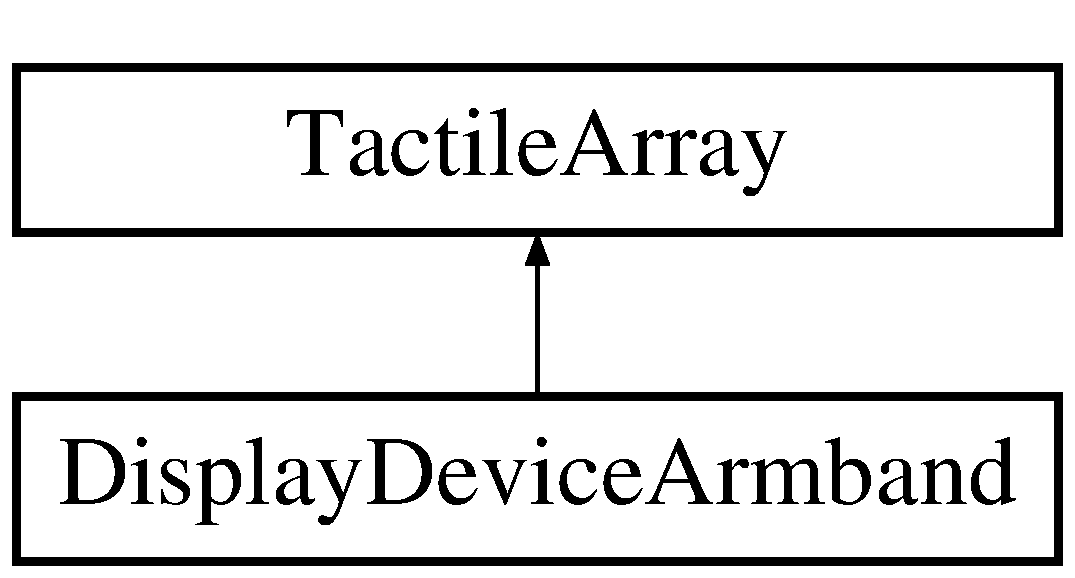
\includegraphics[height=2.000000cm]{classDisplayDeviceArmband}
\end{center}
\end{figure}
\subsection*{Public Member Functions}
\begin{DoxyCompactItemize}
\item 
\hypertarget{classDisplayDeviceArmband_a6fe8bd8b16190fe162a421cc004dc686}{
{\bfseries DisplayDeviceArmband} (int a\_\-portNum)}
\label{classDisplayDeviceArmband_a6fe8bd8b16190fe162a421cc004dc686}

\item 
\hypertarget{classDisplayDeviceArmband_a645221ffbc870f0bb19c659c36722541}{
void {\bfseries setActReset} ()}
\label{classDisplayDeviceArmband_a645221ffbc870f0bb19c659c36722541}

\item 
\hypertarget{classDisplayDeviceArmband_ab213e4b1d2cc70b5ec302ad7835e74f2}{
void {\bfseries setActForearm} (double a\_\-actX, double a\_\-actY)}
\label{classDisplayDeviceArmband_ab213e4b1d2cc70b5ec302ad7835e74f2}

\end{DoxyCompactItemize}
\subsection*{Data Fields}
\begin{DoxyCompactItemize}
\item 
\hypertarget{classDisplayDeviceArmband_a55fb2729682ab7f7a2b290f396099f06}{
int {\bfseries m\_\-array} \mbox{[}ARMBAND\_\-ARRAY\_\-SIZE\_\-X\mbox{]}\mbox{[}ARMBAND\_\-ARRAY\_\-SIZE\_\-Y\mbox{]}}
\label{classDisplayDeviceArmband_a55fb2729682ab7f7a2b290f396099f06}

\end{DoxyCompactItemize}


The documentation for this class was generated from the following files:\begin{DoxyCompactItemize}
\item 
/home/kevin/workspace/HugMe/HugMe v0.9.1/Jacket/DisplayDeviceArmband.h\item 
/home/kevin/workspace/HugMe/HugMe v0.9.1/Jacket/DisplayDeviceArmband.cpp\end{DoxyCompactItemize}

\hypertarget{classDisplayDeviceJacket}{
\section{DisplayDeviceJacket Class Reference}
\label{classDisplayDeviceJacket}\index{DisplayDeviceJacket@{DisplayDeviceJacket}}
}
Inheritance diagram for DisplayDeviceJacket:\begin{figure}[H]
\begin{center}
\leavevmode
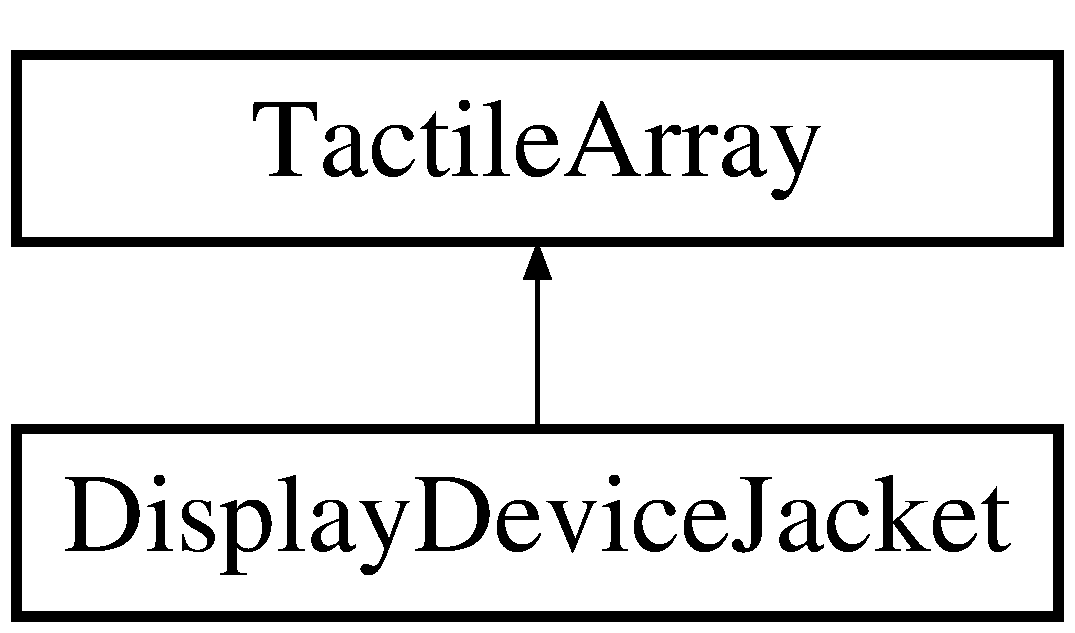
\includegraphics[height=2cm]{classDisplayDeviceJacket}
\end{center}
\end{figure}
\subsection*{Public Member Functions}
\begin{DoxyCompactItemize}
\item 
\hypertarget{classDisplayDeviceJacket_a73dce07052df2ef3703406e3fdf3ef52}{
{\bfseries DisplayDeviceJacket} (int a\_\-portNum)}
\label{classDisplayDeviceJacket_a73dce07052df2ef3703406e3fdf3ef52}

\item 
\hypertarget{classDisplayDeviceJacket_a5b02adb89dc81459d7c869293a9f000a}{
void {\bfseries setActReset} ()}
\label{classDisplayDeviceJacket_a5b02adb89dc81459d7c869293a9f000a}

\item 
\hypertarget{classDisplayDeviceJacket_a1cc7bc19638a4d5e7a00677781952c29}{
void {\bfseries setActChest} (double a\_\-actX, double a\_\-actY)}
\label{classDisplayDeviceJacket_a1cc7bc19638a4d5e7a00677781952c29}

\item 
\hypertarget{classDisplayDeviceJacket_ab8db22ff8bd0069140df975adfe05719}{
void {\bfseries setActUpperArm} (double a\_\-actX, double a\_\-actY)}
\label{classDisplayDeviceJacket_ab8db22ff8bd0069140df975adfe05719}

\item 
\hypertarget{classDisplayDeviceJacket_a86bb0b50805faf6db0493618c3f10973}{
void {\bfseries setActNeck} (int a\_\-actX, double a\_\-intensity)}
\label{classDisplayDeviceJacket_a86bb0b50805faf6db0493618c3f10973}

\end{DoxyCompactItemize}
\subsection*{Data Fields}
\begin{DoxyCompactItemize}
\item 
\hypertarget{classDisplayDeviceJacket_aeeb22dbc14edfa3135d2f2d0dfbd2238}{
int {\bfseries m\_\-chestArray} \mbox{[}CHEST\_\-ARRAY\_\-SIZE\_\-X\mbox{]}\mbox{[}CHEST\_\-ARRAY\_\-SIZE\_\-Y\mbox{]}}
\label{classDisplayDeviceJacket_aeeb22dbc14edfa3135d2f2d0dfbd2238}

\item 
\hypertarget{classDisplayDeviceJacket_a08e1944626872efce9af22ade970b04d}{
int {\bfseries m\_\-armArray} \mbox{[}ARM\_\-ARRAY\_\-SIZE\_\-X\mbox{]}\mbox{[}ARM\_\-ARRAY\_\-SIZE\_\-Y\mbox{]}}
\label{classDisplayDeviceJacket_a08e1944626872efce9af22ade970b04d}

\item 
\hypertarget{classDisplayDeviceJacket_a786295631af23d5b7b970edbd30b4395}{
int {\bfseries m\_\-neckArray} \mbox{[}NECK\_\-ARRAY\_\-SIZE\_\-X\mbox{]}\mbox{[}NECK\_\-ARRAY\_\-SIZE\_\-Y\mbox{]}}
\label{classDisplayDeviceJacket_a786295631af23d5b7b970edbd30b4395}

\end{DoxyCompactItemize}


The documentation for this class was generated from the following files:\begin{DoxyCompactItemize}
\item 
/home/kevin/workspace/HugMe/HugMe v0.9.1/Jacket/DisplayDeviceJacket.h\item 
/home/kevin/workspace/HugMe/HugMe v0.9.1/Jacket/DisplayDeviceJacket.cpp\end{DoxyCompactItemize}

\hypertarget{classFalcon}{
\section{Falcon Class Reference}
\label{classFalcon}\index{Falcon@{Falcon}}
}


Abstract class that represents a falcon.  




{\ttfamily \#include $<$Falcon.h$>$}

Inheritance diagram for Falcon:\begin{figure}[H]
\begin{center}
\leavevmode
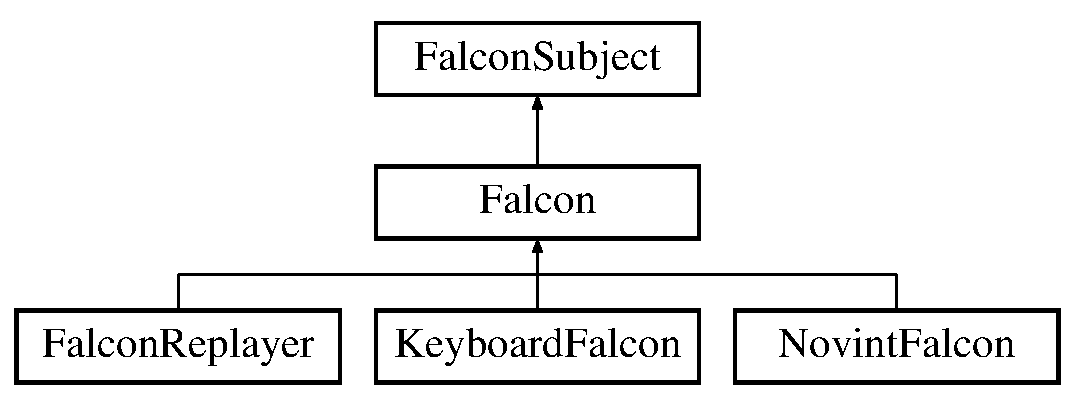
\includegraphics[height=3.000000cm]{classFalcon}
\end{center}
\end{figure}
\subsection*{Public Member Functions}
\begin{DoxyCompactItemize}
\item 
\hypertarget{classFalcon_ae571e7658369b1b4473c5aa75d407299}{
\hyperlink{classFalcon_ae571e7658369b1b4473c5aa75d407299}{Falcon} ()}
\label{classFalcon_ae571e7658369b1b4473c5aa75d407299}

\begin{DoxyCompactList}\small\item\em Constructor. \item\end{DoxyCompactList}\item 
\hypertarget{classFalcon_aae1dd1036d4fde5216a76989f5e02a47}{
virtual \hyperlink{classFalcon_aae1dd1036d4fde5216a76989f5e02a47}{$\sim$Falcon} ()}
\label{classFalcon_aae1dd1036d4fde5216a76989f5e02a47}

\begin{DoxyCompactList}\small\item\em Destructor. \item\end{DoxyCompactList}\item 
\hypertarget{classFalcon_a4de207fe80e98bf959ed7a41dca6012d}{
virtual void \hyperlink{classFalcon_a4de207fe80e98bf959ed7a41dca6012d}{startPolling} ()=0}
\label{classFalcon_a4de207fe80e98bf959ed7a41dca6012d}

\begin{DoxyCompactList}\small\item\em Start polling the falcon for information. \item\end{DoxyCompactList}\item 
\hypertarget{classFalcon_ade1bdf4fb8825aa69927418045227e72}{
virtual void \hyperlink{classFalcon_ade1bdf4fb8825aa69927418045227e72}{stopPolling} ()=0}
\label{classFalcon_ade1bdf4fb8825aa69927418045227e72}

\begin{DoxyCompactList}\small\item\em Stop polling the falcon for information. \item\end{DoxyCompactList}\item 
virtual cCollisionAABBBox \hyperlink{classFalcon_a8113221c67437ed4f726af6d68c0e66e}{boundingBox} () const =0
\begin{DoxyCompactList}\small\item\em Returns the box to which the slingshot is bound. \item\end{DoxyCompactList}\end{DoxyCompactItemize}


\subsection{Detailed Description}
Abstract class that represents a falcon. The falcon will report events such as slingshot movement and slingshot firing. 

\subsection{Member Function Documentation}
\hypertarget{classFalcon_a8113221c67437ed4f726af6d68c0e66e}{
\index{Falcon@{Falcon}!boundingBox@{boundingBox}}
\index{boundingBox@{boundingBox}!Falcon@{Falcon}}
\subsubsection[{boundingBox}]{\setlength{\rightskip}{0pt plus 5cm}virtual cCollisionAABBBox Falcon::boundingBox (
\begin{DoxyParamCaption}
{}
\end{DoxyParamCaption}
) const\hspace{0.3cm}{\ttfamily  \mbox{[}pure virtual\mbox{]}}}}
\label{classFalcon_a8113221c67437ed4f726af6d68c0e66e}


Returns the box to which the slingshot is bound. 

\begin{DoxyReturn}{Returns}
the box to which the slingshot is bound 
\end{DoxyReturn}


Implemented in \hyperlink{classKeyboardFalcon_a5f4b4e7d349e46f2662f8da3baa09086}{KeyboardFalcon}, \hyperlink{classNovintFalcon_a8226c5b4a2cb0d2e88b6a41e2c7c3af9}{NovintFalcon}, and \hyperlink{classFalconReplayer_a9ecce406249112f611f72530e942e881}{FalconReplayer}.



The documentation for this class was generated from the following files:\begin{DoxyCompactItemize}
\item 
/home/kevin/workspace/HugMe/HugMe v0.9.1/Falcon/Falcon.h\item 
/home/kevin/workspace/HugMe/HugMe v0.9.1/Falcon/Falcon.cpp\end{DoxyCompactItemize}

\hypertarget{classFalconObserver}{
\section{FalconObserver Class Reference}
\label{classFalconObserver}\index{FalconObserver@{FalconObserver}}
}
Inheritance diagram for FalconObserver:\begin{figure}[H]
\begin{center}
\leavevmode
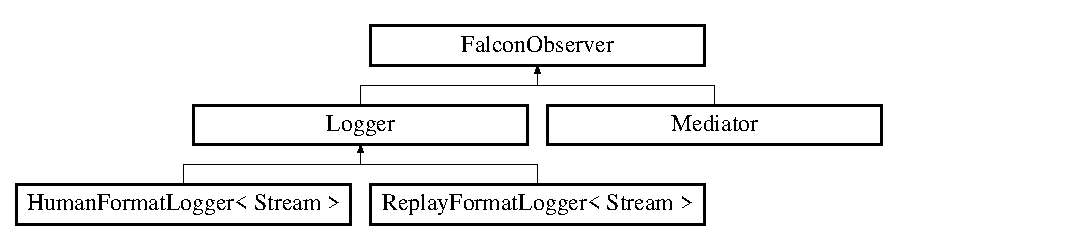
\includegraphics[height=2.78607cm]{classFalconObserver}
\end{center}
\end{figure}
\subsection*{Public Member Functions}
\begin{DoxyCompactItemize}
\item 
\hypertarget{classFalconObserver_a6a6dd6934aefdb9de8e94b089b21e1b9}{
virtual void {\bfseries update} (FalconUpdateContext context, const void $\ast$data)=0}
\label{classFalconObserver_a6a6dd6934aefdb9de8e94b089b21e1b9}

\end{DoxyCompactItemize}


The documentation for this class was generated from the following files:\begin{DoxyCompactItemize}
\item 
/home/kevin/workspace/HugMe/HugMe v0.9.1/Falcon/FalconObserver.h\item 
/home/kevin/workspace/HugMe/HugMe v0.9.1/Falcon/FalconObserver.cpp\end{DoxyCompactItemize}

\hypertarget{classFalconReplayer}{
\section{FalconReplayer Class Reference}
\label{classFalconReplayer}\index{FalconReplayer@{FalconReplayer}}
}
Inheritance diagram for FalconReplayer:\begin{figure}[H]
\begin{center}
\leavevmode
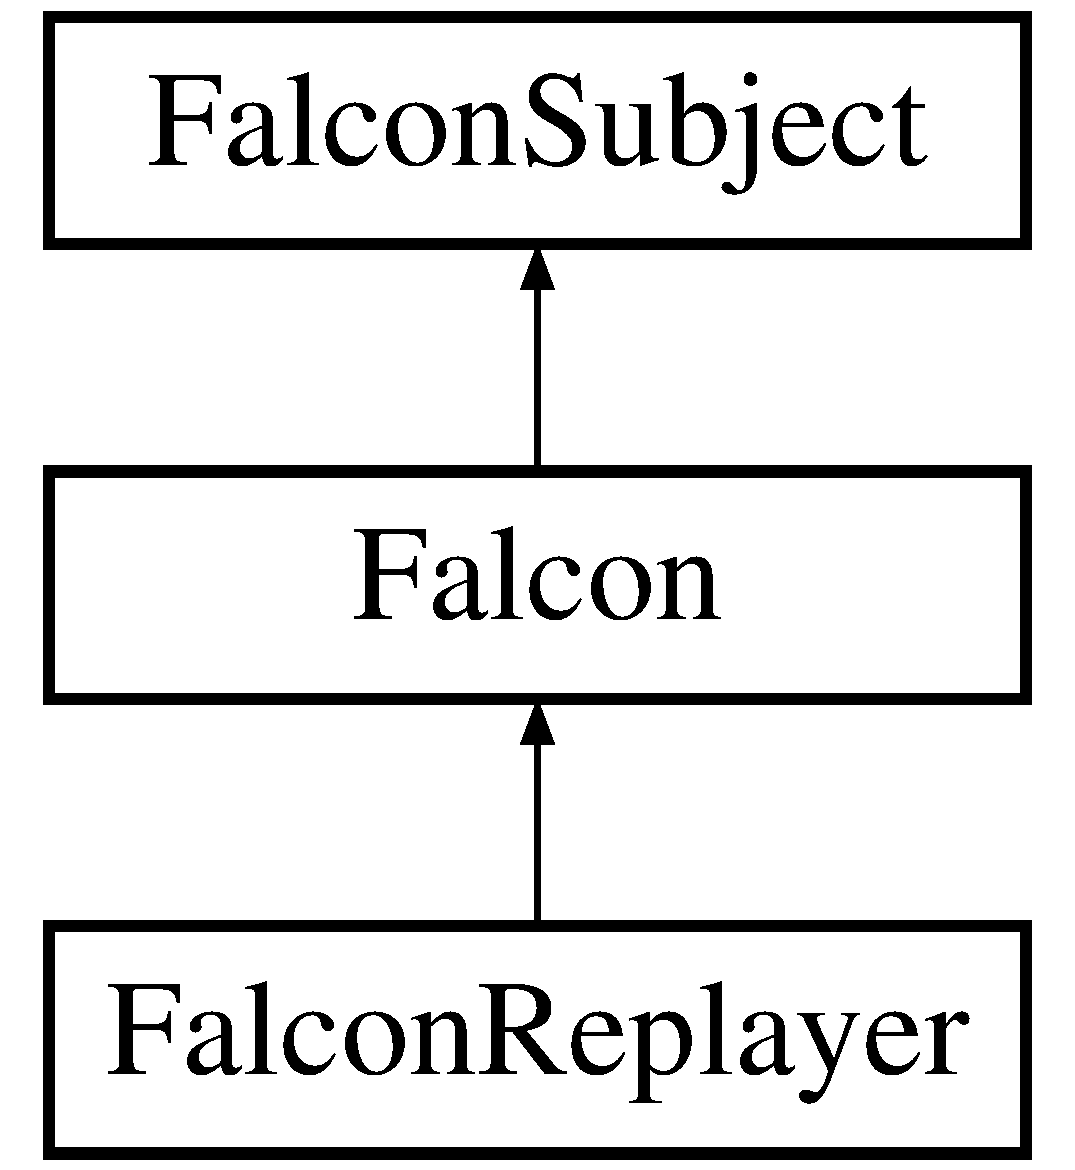
\includegraphics[height=3.000000cm]{classFalconReplayer}
\end{center}
\end{figure}
\subsection*{Public Member Functions}
\begin{DoxyCompactItemize}
\item 
\hypertarget{classFalconReplayer_a8b0921f53e7c34181b9ee8120070acea}{
{\bfseries FalconReplayer} (boost::shared\_\-ptr$<$ std::ifstream $>$ file, boost::shared\_\-ptr$<$ boost::archive::text\_\-iarchive $>$ archive)}
\label{classFalconReplayer_a8b0921f53e7c34181b9ee8120070acea}

\item 
\hypertarget{classFalconReplayer_a831a6e87b2497f0c1af4bc7fd5ed7d54}{
void {\bfseries replay} (LogEvent\_\-t logEvent)}
\label{classFalconReplayer_a831a6e87b2497f0c1af4bc7fd5ed7d54}

\item 
\hypertarget{classFalconReplayer_ad75b679b3c287c4d53041988e7a0ab45}{
virtual void \hyperlink{classFalconReplayer_ad75b679b3c287c4d53041988e7a0ab45}{startPolling} ()}
\label{classFalconReplayer_ad75b679b3c287c4d53041988e7a0ab45}

\begin{DoxyCompactList}\small\item\em Start polling the falcon for information. \item\end{DoxyCompactList}\item 
\hypertarget{classFalconReplayer_a1487ef2142d0a4748f44f78e1356cffa}{
virtual void \hyperlink{classFalconReplayer_a1487ef2142d0a4748f44f78e1356cffa}{stopPolling} ()}
\label{classFalconReplayer_a1487ef2142d0a4748f44f78e1356cffa}

\begin{DoxyCompactList}\small\item\em Stop polling the falcon for information. \item\end{DoxyCompactList}\item 
virtual cCollisionAABBBox \hyperlink{classFalconReplayer_a9ecce406249112f611f72530e942e881}{boundingBox} () const 
\begin{DoxyCompactList}\small\item\em Returns the box to which the slingshot is bound. \item\end{DoxyCompactList}\end{DoxyCompactItemize}


\subsection{Member Function Documentation}
\hypertarget{classFalconReplayer_a9ecce406249112f611f72530e942e881}{
\index{FalconReplayer@{FalconReplayer}!boundingBox@{boundingBox}}
\index{boundingBox@{boundingBox}!FalconReplayer@{FalconReplayer}}
\subsubsection[{boundingBox}]{\setlength{\rightskip}{0pt plus 5cm}cCollisionAABBBox FalconReplayer::boundingBox (
\begin{DoxyParamCaption}
{}
\end{DoxyParamCaption}
) const\hspace{0.3cm}{\ttfamily  \mbox{[}virtual\mbox{]}}}}
\label{classFalconReplayer_a9ecce406249112f611f72530e942e881}


Returns the box to which the slingshot is bound. 

\begin{DoxyReturn}{Returns}
the box to which the slingshot is bound 
\end{DoxyReturn}


Implements \hyperlink{classFalcon_a8113221c67437ed4f726af6d68c0e66e}{Falcon}.



The documentation for this class was generated from the following files:\begin{DoxyCompactItemize}
\item 
/home/kevin/workspace/HugMe/HugMe v0.9.1/Replay/FalconReplayer.h\item 
/home/kevin/workspace/HugMe/HugMe v0.9.1/Replay/FalconReplayer.cpp\end{DoxyCompactItemize}

\hypertarget{classFalconSubject}{
\section{FalconSubject Class Reference}
\label{classFalconSubject}\index{FalconSubject@{FalconSubject}}
}


Abstract class in the observer pattern for the falcon.  




{\ttfamily \#include $<$FalconSubject.h$>$}

Inheritance diagram for FalconSubject:\begin{figure}[H]
\begin{center}
\leavevmode
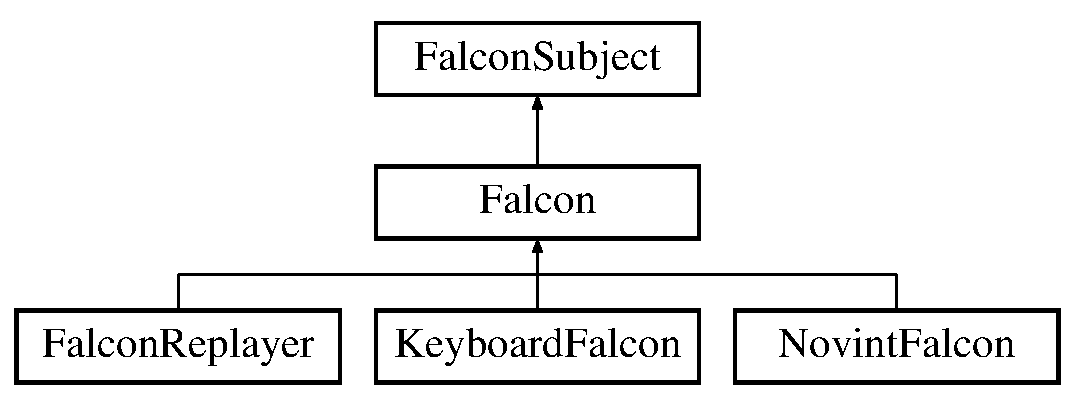
\includegraphics[height=3.000000cm]{classFalconSubject}
\end{center}
\end{figure}
\subsection*{Public Member Functions}
\begin{DoxyCompactItemize}
\item 
\hypertarget{classFalconSubject_a1c7a53a4d28fbb83d305fd62470bfaa2}{
\hyperlink{classFalconSubject_a1c7a53a4d28fbb83d305fd62470bfaa2}{FalconSubject} ()}
\label{classFalconSubject_a1c7a53a4d28fbb83d305fd62470bfaa2}

\begin{DoxyCompactList}\small\item\em Constructor. \item\end{DoxyCompactList}\item 
\hypertarget{classFalconSubject_afd64db787e2371dc09b73917209f3566}{
virtual \hyperlink{classFalconSubject_afd64db787e2371dc09b73917209f3566}{$\sim$FalconSubject} ()}
\label{classFalconSubject_afd64db787e2371dc09b73917209f3566}

\begin{DoxyCompactList}\small\item\em Destructor. \item\end{DoxyCompactList}\item 
void \hyperlink{classFalconSubject_a081d12a24abd16b88b69230f82ce1ec7}{attach} (\hyperlink{classFalconObserver}{FalconObserver} $\ast$observer)
\begin{DoxyCompactList}\small\item\em Attach a new observer to this subject. \item\end{DoxyCompactList}\item 
void \hyperlink{classFalconSubject_aaa69f14bf9659f783b9d95da47e55868}{detach} (\hyperlink{classFalconObserver}{FalconObserver} $\ast$observer)
\begin{DoxyCompactList}\small\item\em Detach an observer from this subject. \item\end{DoxyCompactList}\item 
void \hyperlink{classFalconSubject_abd19e56b3ffb433705576e361cc5b28f}{notify} (FalconUpdateContext context, const void $\ast$data=NULL)
\begin{DoxyCompactList}\small\item\em Notifies all observers that a new update is available. \item\end{DoxyCompactList}\end{DoxyCompactItemize}


\subsection{Detailed Description}
Abstract class in the observer pattern for the falcon. This class is used to report falcon related updates to the observers. 

\subsection{Member Function Documentation}
\hypertarget{classFalconSubject_a081d12a24abd16b88b69230f82ce1ec7}{
\index{FalconSubject@{FalconSubject}!attach@{attach}}
\index{attach@{attach}!FalconSubject@{FalconSubject}}
\subsubsection[{attach}]{\setlength{\rightskip}{0pt plus 5cm}void FalconSubject::attach (
\begin{DoxyParamCaption}
\item[{{\bf FalconObserver} $\ast$}]{ observer}
\end{DoxyParamCaption}
)}}
\label{classFalconSubject_a081d12a24abd16b88b69230f82ce1ec7}


Attach a new observer to this subject. 


\begin{DoxyParams}{Parameters}
\item[{\em observer}]The observer to attach to this subject. No duplicated are allowed. \end{DoxyParams}
\hypertarget{classFalconSubject_aaa69f14bf9659f783b9d95da47e55868}{
\index{FalconSubject@{FalconSubject}!detach@{detach}}
\index{detach@{detach}!FalconSubject@{FalconSubject}}
\subsubsection[{detach}]{\setlength{\rightskip}{0pt plus 5cm}void FalconSubject::detach (
\begin{DoxyParamCaption}
\item[{{\bf FalconObserver} $\ast$}]{ observer}
\end{DoxyParamCaption}
)}}
\label{classFalconSubject_aaa69f14bf9659f783b9d95da47e55868}


Detach an observer from this subject. 


\begin{DoxyParams}{Parameters}
\item[{\em observer}]The observer to detach from this subject. \end{DoxyParams}
\hypertarget{classFalconSubject_abd19e56b3ffb433705576e361cc5b28f}{
\index{FalconSubject@{FalconSubject}!notify@{notify}}
\index{notify@{notify}!FalconSubject@{FalconSubject}}
\subsubsection[{notify}]{\setlength{\rightskip}{0pt plus 5cm}void FalconSubject::notify (
\begin{DoxyParamCaption}
\item[{FalconUpdateContext}]{ context, }
\item[{const void $\ast$}]{ data = {\ttfamily NULL}}
\end{DoxyParamCaption}
)}}
\label{classFalconSubject_abd19e56b3ffb433705576e361cc5b28f}


Notifies all observers that a new update is available. 


\begin{DoxyParams}{Parameters}
\item[{\em context}]The context of the update, ex: slingshot moved. \item[{\em data}]The data associated with the update, ex: the slingshot's new position. \end{DoxyParams}


The documentation for this class was generated from the following files:\begin{DoxyCompactItemize}
\item 
/home/kevin/workspace/HugMe/HugMe v0.9.1/Falcon/FalconSubject.h\item 
/home/kevin/workspace/HugMe/HugMe v0.9.1/Falcon/FalconSubject.cpp\end{DoxyCompactItemize}

\hypertarget{classGame}{
\section{Game Class Reference}
\label{classGame}\index{Game@{Game}}
}


Represents the \hyperlink{classOfficeSlingshot3D}{OfficeSlingshot3D} game.  




{\ttfamily \#include $<$Game.h$>$}

Inheritance diagram for Game:\begin{figure}[H]
\begin{center}
\leavevmode
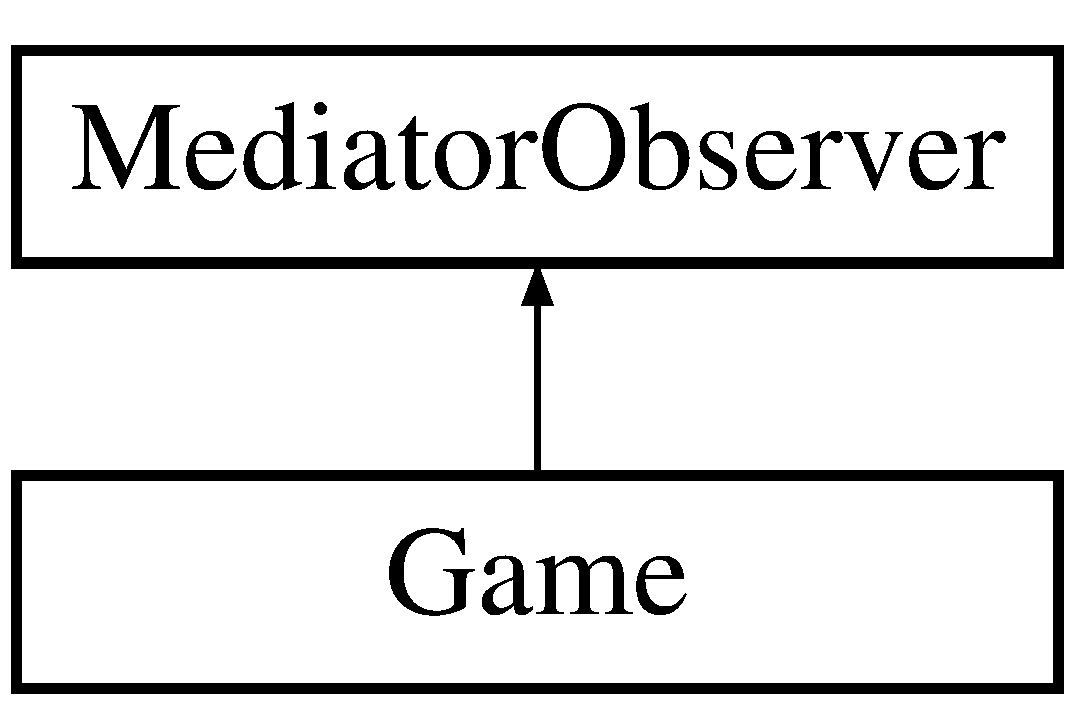
\includegraphics[height=2.000000cm]{classGame}
\end{center}
\end{figure}
\subsection*{Public Member Functions}
\begin{DoxyCompactItemize}
\item 
\hypertarget{classGame_ae4a3e825c02c218e3a110586dbc964f5}{
\hyperlink{classGame_ae4a3e825c02c218e3a110586dbc964f5}{Game} (boost::shared\_\-ptr$<$ \hyperlink{classMediator}{Mediator} $>$ mediator)}
\label{classGame_ae4a3e825c02c218e3a110586dbc964f5}

\begin{DoxyCompactList}\small\item\em Constructor. \item\end{DoxyCompactList}\item 
\hypertarget{classGame_ae3d112ca6e0e55150d2fdbc704474530}{
virtual \hyperlink{classGame_ae3d112ca6e0e55150d2fdbc704474530}{$\sim$Game} ()}
\label{classGame_ae3d112ca6e0e55150d2fdbc704474530}

\begin{DoxyCompactList}\small\item\em Destructor. \item\end{DoxyCompactList}\item 
\hypertarget{classGame_a1e83402bc85f4ef4150bee568e4f8986}{
virtual void \hyperlink{classGame_a1e83402bc85f4ef4150bee568e4f8986}{update} (\hyperlink{namespaceMediatorUpdateContext_aa3a9bed543f2a2237dc2b6feea170a1d}{MediatorUpdateContext\_\-t} context, const void $\ast$data)}
\label{classGame_a1e83402bc85f4ef4150bee568e4f8986}

\begin{DoxyCompactList}\small\item\em Updates from the mediator. \item\end{DoxyCompactList}\end{DoxyCompactItemize}


\subsection{Detailed Description}
Represents the \hyperlink{classOfficeSlingshot3D}{OfficeSlingshot3D} game. Holds game data (score, health, etc ...) and the games 3d representation. 

The documentation for this class was generated from the following files:\begin{DoxyCompactItemize}
\item 
/home/kevin/workspace/HugMe/HugMe v0.9.1/Game/Game.h\item 
/home/kevin/workspace/HugMe/HugMe v0.9.1/Game/Game.cpp\end{DoxyCompactItemize}

\hypertarget{classHpBar}{
\section{HpBar Class Reference}
\label{classHpBar}\index{HpBar@{HpBar}}
}
\subsection*{Public Member Functions}
\begin{DoxyCompactItemize}
\item 
\hypertarget{classHpBar_ab7308dcda24cad121b9eea5f16f0196d}{
{\bfseries HpBar} (cWorld $\ast$world, bool isLocal)}
\label{classHpBar_ab7308dcda24cad121b9eea5f16f0196d}

\item 
\hypertarget{classHpBar_a2d64d6ec33cd462d243e0ebf910f6dcf}{
void {\bfseries ReduceHP} (int hpLost)}
\label{classHpBar_a2d64d6ec33cd462d243e0ebf910f6dcf}

\end{DoxyCompactItemize}


The documentation for this class was generated from the following files:\begin{DoxyCompactItemize}
\item 
/home/kevin/workspace/HugMe/HugMe v0.9.1/Game/HpBar.h\item 
/home/kevin/workspace/HugMe/HugMe v0.9.1/Game/HpBar.cpp\end{DoxyCompactItemize}

\hypertarget{classHumanFormatLogger}{
\section{HumanFormatLogger$<$ Stream $>$ Class Template Reference}
\label{classHumanFormatLogger}\index{HumanFormatLogger@{HumanFormatLogger}}
}
Inheritance diagram for HumanFormatLogger$<$ Stream $>$:\begin{figure}[H]
\begin{center}
\leavevmode
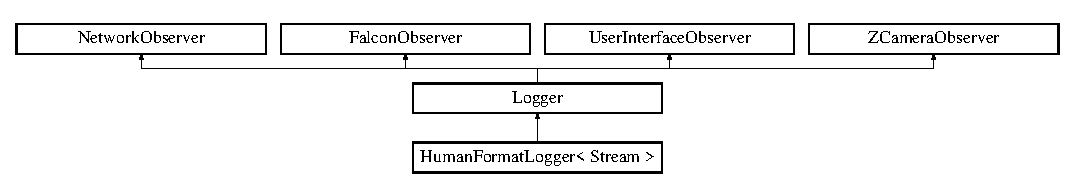
\includegraphics[height=1.67164cm]{classHumanFormatLogger}
\end{center}
\end{figure}
\subsection*{Public Member Functions}
\begin{DoxyCompactItemize}
\item 
\hypertarget{classHumanFormatLogger_a404b51267a3478a726242290a9515bda}{
{\footnotesize template$<$typename T1 $>$ }\\{\bfseries HumanFormatLogger} (T1 param)}
\label{classHumanFormatLogger_a404b51267a3478a726242290a9515bda}

\item 
\hypertarget{classHumanFormatLogger_ae8bb78a585c0870cf9b60012631414d4}{
{\footnotesize template$<$typename T1 , typename T2 $>$ }\\{\bfseries HumanFormatLogger} (T1 param1, T2 param2)}
\label{classHumanFormatLogger_ae8bb78a585c0870cf9b60012631414d4}

\item 
\hypertarget{classHumanFormatLogger_ad8fa4b5491db92d554d3eebdb318c72e}{
{\footnotesize template$<$typename T1 , typename T2 , typename T3 $>$ }\\{\bfseries HumanFormatLogger} (T1 param1, T2 param2, T3 param3)}
\label{classHumanFormatLogger_ad8fa4b5491db92d554d3eebdb318c72e}

\end{DoxyCompactItemize}
\subsection*{Protected Member Functions}
\begin{DoxyCompactItemize}
\item 
\hypertarget{classHumanFormatLogger_a36ded631f6095de7b0cb96ec2af0944c}{
virtual void {\bfseries log} (LogEvent\_\-t logEvent)}
\label{classHumanFormatLogger_a36ded631f6095de7b0cb96ec2af0944c}

\item 
\hypertarget{classHumanFormatLogger_a2e419cfe25dbf748ee6b0eb2141f65fc}{
virtual void {\bfseries log} (LogEvent\_\-t logEvent, rc\_\-network error)}
\label{classHumanFormatLogger_a2e419cfe25dbf748ee6b0eb2141f65fc}

\item 
\hypertarget{classHumanFormatLogger_adce37538632ef3b2eb7527e49a31d818}{
virtual void {\bfseries log} (LogEvent\_\-t logEvent, const std::string \&str)}
\label{classHumanFormatLogger_adce37538632ef3b2eb7527e49a31d818}

\item 
\hypertarget{classHumanFormatLogger_a69901184b8637645606705513f7dbc3e}{
virtual void {\bfseries log} (LogEvent\_\-t logEvent, const \hyperlink{structVideoData}{VideoData} \&video)}
\label{classHumanFormatLogger_a69901184b8637645606705513f7dbc3e}

\item 
\hypertarget{classHumanFormatLogger_ace0b4baa6c6999ca4111e4bc443e6b4a}{
virtual void {\bfseries log} (LogEvent\_\-t logEvent, const cVector3d \&vec)}
\label{classHumanFormatLogger_ace0b4baa6c6999ca4111e4bc443e6b4a}

\item 
\hypertarget{classHumanFormatLogger_a84e429003498dc59385e7e4dfd4dee64}{
virtual void {\bfseries log} (LogEvent\_\-t logEvent, const \hyperlink{classProjectile}{Projectile} \&projectile)}
\label{classHumanFormatLogger_a84e429003498dc59385e7e4dfd4dee64}

\item 
\hypertarget{classHumanFormatLogger_a3ef78598907255bd9a467932f523d2fb}{
virtual void {\bfseries log} (LogEvent\_\-t logEvent, const \hyperlink{structUserPreferences}{UserPreferences} \&preferences)}
\label{classHumanFormatLogger_a3ef78598907255bd9a467932f523d2fb}

\end{DoxyCompactItemize}
\subsubsection*{template$<$typename Stream$>$ class HumanFormatLogger$<$ Stream $>$}



The documentation for this class was generated from the following file:\begin{DoxyCompactItemize}
\item 
/home/kevin/workspace/HugMe/HugMe v0.9.1/Logger/HumanFormatLogger.h\end{DoxyCompactItemize}

\hypertarget{classIZCamera}{
\section{IZCamera Class Reference}
\label{classIZCamera}\index{IZCamera@{IZCamera}}
}
Inheritance diagram for IZCamera:\begin{figure}[H]
\begin{center}
\leavevmode
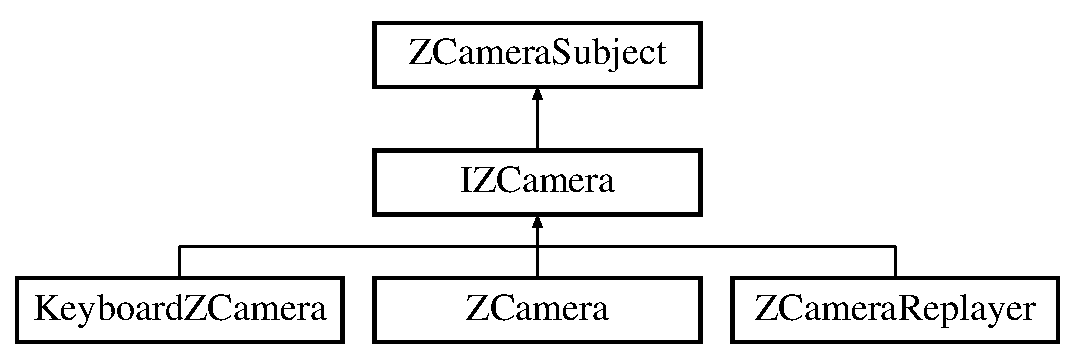
\includegraphics[height=3cm]{classIZCamera}
\end{center}
\end{figure}
\subsection*{Public Member Functions}
\begin{DoxyCompactItemize}
\item 
\hypertarget{classIZCamera_a6d9b10985172343983a9edbdb324c367}{
virtual void {\bfseries startCapture} ()=0}
\label{classIZCamera_a6d9b10985172343983a9edbdb324c367}

\item 
\hypertarget{classIZCamera_ac1a752c869fc2c97b0f7feff6163068f}{
virtual void {\bfseries stopCapture} ()=0}
\label{classIZCamera_ac1a752c869fc2c97b0f7feff6163068f}

\end{DoxyCompactItemize}


The documentation for this class was generated from the following files:\begin{DoxyCompactItemize}
\item 
/home/kevin/workspace/HugMe/HugMe v0.9.1/ZCamera/IZCamera.h\item 
/home/kevin/workspace/HugMe/HugMe v0.9.1/ZCamera/IZCamera.cpp\end{DoxyCompactItemize}

\hypertarget{classKeyboardFalcon}{
\section{KeyboardFalcon Class Reference}
\label{classKeyboardFalcon}\index{KeyboardFalcon@{KeyboardFalcon}}
}


\hyperlink{classFalcon}{Falcon} emulator that uses the keyboard instead of a novint falcon.  




{\ttfamily \#include $<$KeyboardFalcon.h$>$}

Inheritance diagram for KeyboardFalcon:\begin{figure}[H]
\begin{center}
\leavevmode
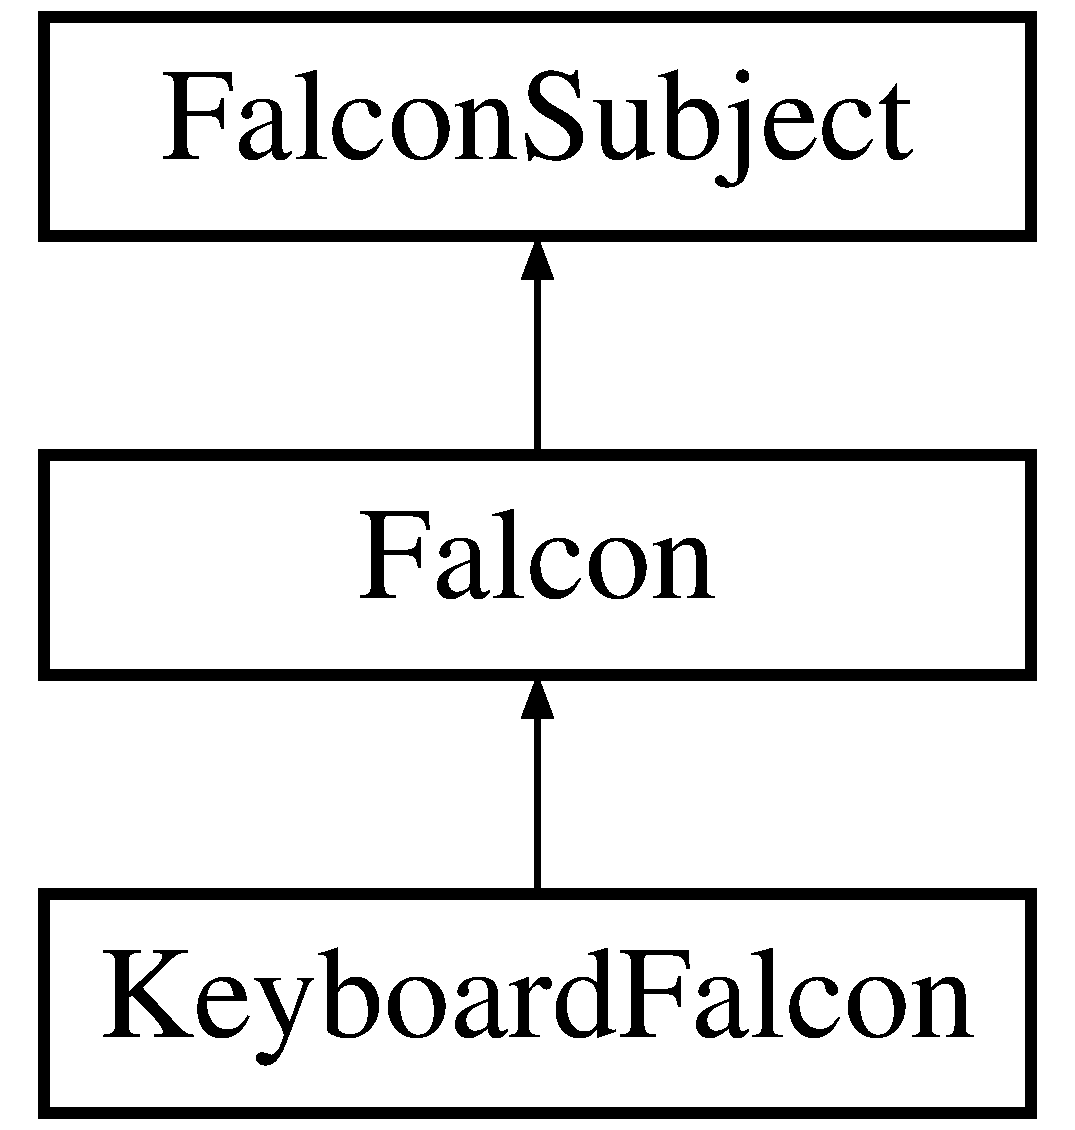
\includegraphics[height=3.000000cm]{classKeyboardFalcon}
\end{center}
\end{figure}
\subsection*{Public Member Functions}
\begin{DoxyCompactItemize}
\item 
\hypertarget{classKeyboardFalcon_a7b79d2129b322900cc65f6f250469875}{
\hyperlink{classKeyboardFalcon_a7b79d2129b322900cc65f6f250469875}{KeyboardFalcon} ()}
\label{classKeyboardFalcon_a7b79d2129b322900cc65f6f250469875}

\begin{DoxyCompactList}\small\item\em Constructor. \item\end{DoxyCompactList}\item 
\hypertarget{classKeyboardFalcon_a1db3b6a58d955521253dfc7067a88f36}{
virtual \hyperlink{classKeyboardFalcon_a1db3b6a58d955521253dfc7067a88f36}{$\sim$KeyboardFalcon} ()}
\label{classKeyboardFalcon_a1db3b6a58d955521253dfc7067a88f36}

\begin{DoxyCompactList}\small\item\em Destructor. \item\end{DoxyCompactList}\item 
\hypertarget{classKeyboardFalcon_af9a2c400cb05910d806861eb8af566f9}{
virtual void \hyperlink{classKeyboardFalcon_af9a2c400cb05910d806861eb8af566f9}{startPolling} ()}
\label{classKeyboardFalcon_af9a2c400cb05910d806861eb8af566f9}

\begin{DoxyCompactList}\small\item\em Start reporting falcon events to the mediator. \item\end{DoxyCompactList}\item 
\hypertarget{classKeyboardFalcon_adf5bf86dd3610843b0db8b8795f6049b}{
virtual void \hyperlink{classKeyboardFalcon_adf5bf86dd3610843b0db8b8795f6049b}{stopPolling} ()}
\label{classKeyboardFalcon_adf5bf86dd3610843b0db8b8795f6049b}

\begin{DoxyCompactList}\small\item\em Stop reporting falcon events to the mediator. \item\end{DoxyCompactList}\item 
\hypertarget{classKeyboardFalcon_a496423ca690aa227530ac8e3f4ce06a0}{
virtual void \hyperlink{classKeyboardFalcon_a496423ca690aa227530ac8e3f4ce06a0}{keyPressed} (unsigned int key)}
\label{classKeyboardFalcon_a496423ca690aa227530ac8e3f4ce06a0}

\begin{DoxyCompactList}\small\item\em Handle a key pressed event. \item\end{DoxyCompactList}\item 
virtual cCollisionAABBBox \hyperlink{classKeyboardFalcon_a5f4b4e7d349e46f2662f8da3baa09086}{boundingBox} () const 
\begin{DoxyCompactList}\small\item\em Returns the box to which the slingshot is bound. \item\end{DoxyCompactList}\end{DoxyCompactItemize}


\subsection{Detailed Description}
\hyperlink{classFalcon}{Falcon} emulator that uses the keyboard instead of a novint falcon. This class should mainly be used for testing purposes as we only have 1 falcon. 

\subsection{Member Function Documentation}
\hypertarget{classKeyboardFalcon_a5f4b4e7d349e46f2662f8da3baa09086}{
\index{KeyboardFalcon@{KeyboardFalcon}!boundingBox@{boundingBox}}
\index{boundingBox@{boundingBox}!KeyboardFalcon@{KeyboardFalcon}}
\subsubsection[{boundingBox}]{\setlength{\rightskip}{0pt plus 5cm}cCollisionAABBBox KeyboardFalcon::boundingBox (
\begin{DoxyParamCaption}
{}
\end{DoxyParamCaption}
) const\hspace{0.3cm}{\ttfamily  \mbox{[}virtual\mbox{]}}}}
\label{classKeyboardFalcon_a5f4b4e7d349e46f2662f8da3baa09086}


Returns the box to which the slingshot is bound. 

\begin{DoxyReturn}{Returns}
the box to which the slingshot is bound 
\end{DoxyReturn}


Implements \hyperlink{classFalcon_a8113221c67437ed4f726af6d68c0e66e}{Falcon}.



The documentation for this class was generated from the following files:\begin{DoxyCompactItemize}
\item 
/home/kevin/workspace/HugMe/HugMe v0.9.1/Falcon/KeyboardFalcon.h\item 
/home/kevin/workspace/HugMe/HugMe v0.9.1/Falcon/KeyboardFalcon.cpp\end{DoxyCompactItemize}

\hypertarget{classKeyboardZCamera}{
\section{KeyboardZCamera Class Reference}
\label{classKeyboardZCamera}\index{KeyboardZCamera@{KeyboardZCamera}}
}


\hyperlink{classZCamera}{ZCamera} emulator that uses the keyboard instead of a z-\/camera.  




{\ttfamily \#include $<$KeyboardZCamera.h$>$}

Inheritance diagram for KeyboardZCamera:\begin{figure}[H]
\begin{center}
\leavevmode
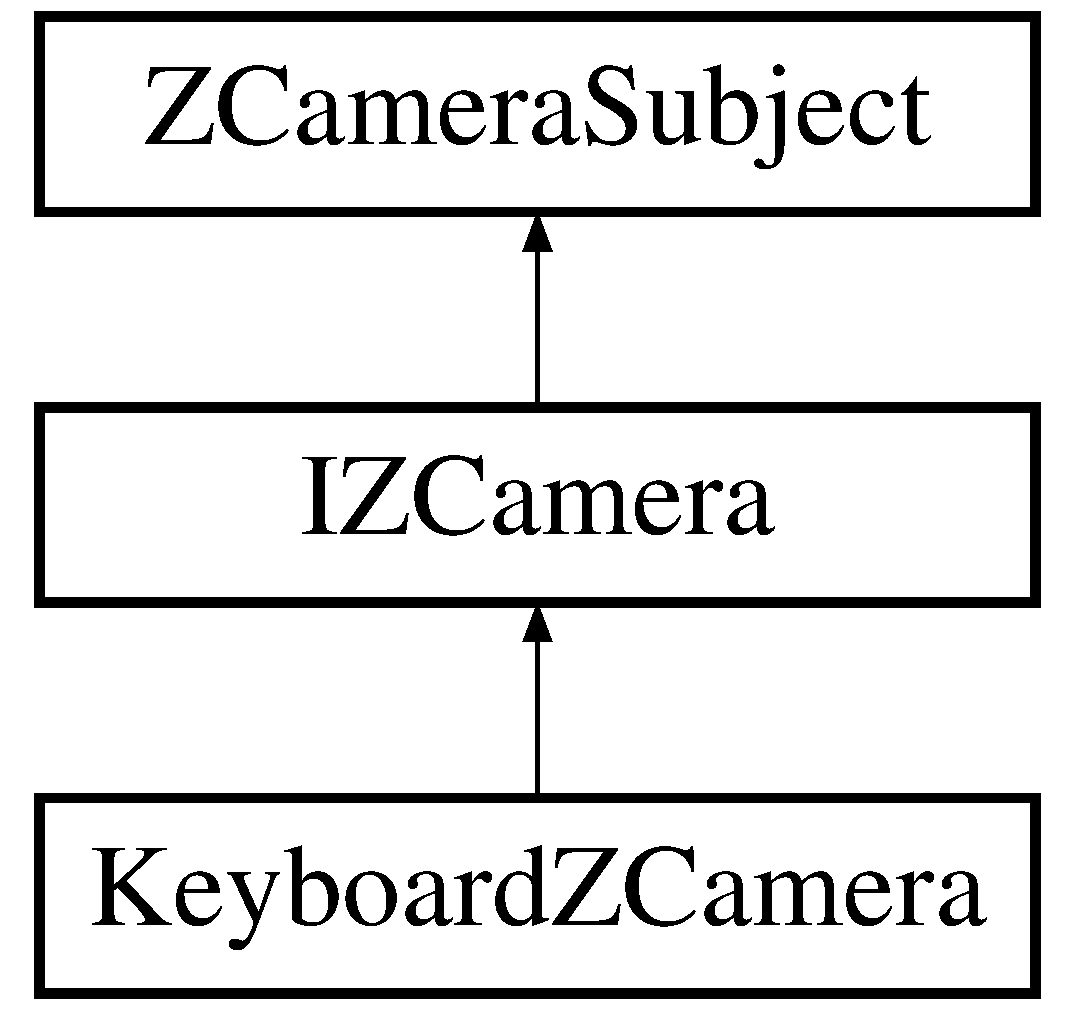
\includegraphics[height=3.000000cm]{classKeyboardZCamera}
\end{center}
\end{figure}
\subsection*{Public Member Functions}
\begin{DoxyCompactItemize}
\item 
\hypertarget{classKeyboardZCamera_a841092440fecfa434ea56764c25ecf13}{
\hyperlink{classKeyboardZCamera_a841092440fecfa434ea56764c25ecf13}{KeyboardZCamera} ()}
\label{classKeyboardZCamera_a841092440fecfa434ea56764c25ecf13}

\begin{DoxyCompactList}\small\item\em Constructor. \item\end{DoxyCompactList}\item 
\hypertarget{classKeyboardZCamera_aec1ca833ec96488fb639de9d70c019b5}{
virtual \hyperlink{classKeyboardZCamera_aec1ca833ec96488fb639de9d70c019b5}{$\sim$KeyboardZCamera} ()}
\label{classKeyboardZCamera_aec1ca833ec96488fb639de9d70c019b5}

\begin{DoxyCompactList}\small\item\em Destructor. \item\end{DoxyCompactList}\item 
\hypertarget{classKeyboardZCamera_a58ab32d15b54521d29dbb538d462d49e}{
virtual void \hyperlink{classKeyboardZCamera_a58ab32d15b54521d29dbb538d462d49e}{startCapture} ()}
\label{classKeyboardZCamera_a58ab32d15b54521d29dbb538d462d49e}

\begin{DoxyCompactList}\small\item\em Start reporting camera events to the mediator. \item\end{DoxyCompactList}\item 
\hypertarget{classKeyboardZCamera_ad8e4f0a5c2c1d5e351231e11f32b0e44}{
virtual void \hyperlink{classKeyboardZCamera_ad8e4f0a5c2c1d5e351231e11f32b0e44}{stopCapture} ()}
\label{classKeyboardZCamera_ad8e4f0a5c2c1d5e351231e11f32b0e44}

\begin{DoxyCompactList}\small\item\em Stop reporting camera events to the mediator. \item\end{DoxyCompactList}\item 
\hypertarget{classKeyboardZCamera_aa939d58755a9b40da1339dfed4fcb5c0}{
virtual void \hyperlink{classKeyboardZCamera_aa939d58755a9b40da1339dfed4fcb5c0}{keyPressed} (unsigned int key)}
\label{classKeyboardZCamera_aa939d58755a9b40da1339dfed4fcb5c0}

\begin{DoxyCompactList}\small\item\em Handle a key pressed event. \item\end{DoxyCompactList}\end{DoxyCompactItemize}


\subsection{Detailed Description}
\hyperlink{classZCamera}{ZCamera} emulator that uses the keyboard instead of a z-\/camera. 

The documentation for this class was generated from the following files:\begin{DoxyCompactItemize}
\item 
/home/kevin/workspace/HugMe/HugMe v0.9.1/ZCamera/KeyboardZCamera.h\item 
/home/kevin/workspace/HugMe/HugMe v0.9.1/ZCamera/KeyboardZCamera.cpp\end{DoxyCompactItemize}

\hypertarget{classLogger}{
\section{Logger Class Reference}
\label{classLogger}\index{Logger@{Logger}}
}
Inheritance diagram for Logger:\begin{figure}[H]
\begin{center}
\leavevmode
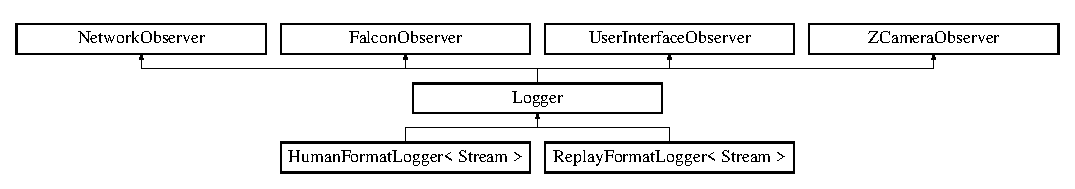
\includegraphics[height=1.67164cm]{classLogger}
\end{center}
\end{figure}
\subsection*{Public Member Functions}
\begin{DoxyCompactItemize}
\item 
\hypertarget{classLogger_abb5098f19a132e91034a6974ed1f2e51}{
virtual void {\bfseries update} (NetworkUpdateContext context, const void $\ast$data)}
\label{classLogger_abb5098f19a132e91034a6974ed1f2e51}

\item 
\hypertarget{classLogger_ab346038a6b7f284d8f57d1296dd98079}{
virtual void {\bfseries update} (UserInterfaceUpdateContext context, const void $\ast$data)}
\label{classLogger_ab346038a6b7f284d8f57d1296dd98079}

\item 
\hypertarget{classLogger_afe25b23b7f952e183f1361ac572800c4}{
virtual void {\bfseries update} (FalconUpdateContext context, const void $\ast$data)}
\label{classLogger_afe25b23b7f952e183f1361ac572800c4}

\item 
\hypertarget{classLogger_a812b14b0d0d04bdc2b30f73bf84790bb}{
virtual void {\bfseries update} (GameUpdateContext context, const void $\ast$data)}
\label{classLogger_a812b14b0d0d04bdc2b30f73bf84790bb}

\item 
\hypertarget{classLogger_a9ac2396edcab7a8ff751bc3bd5a1dd33}{
virtual void {\bfseries update} (ZCameraUpdateContext context, const void $\ast$data)}
\label{classLogger_a9ac2396edcab7a8ff751bc3bd5a1dd33}

\end{DoxyCompactItemize}
\subsection*{Protected Member Functions}
\begin{DoxyCompactItemize}
\item 
\hypertarget{classLogger_a801f41e68772457e9635c68e951cc0f1}{
virtual void {\bfseries log} (LogEvent\_\-t logEvent)=0}
\label{classLogger_a801f41e68772457e9635c68e951cc0f1}

\item 
\hypertarget{classLogger_a2c18b2cbcb7338768d69fc710e1553f5}{
virtual void {\bfseries log} (LogEvent\_\-t logEvent, rc\_\-network error)=0}
\label{classLogger_a2c18b2cbcb7338768d69fc710e1553f5}

\item 
\hypertarget{classLogger_a33d4f1b5211dccdf685210244ccbed15}{
virtual void {\bfseries log} (LogEvent\_\-t logEvent, const std::string \&str)=0}
\label{classLogger_a33d4f1b5211dccdf685210244ccbed15}

\item 
\hypertarget{classLogger_aa7be835d8810ab03f57d11c040ed01ee}{
virtual void {\bfseries log} (LogEvent\_\-t logEvent, const \hyperlink{structVideoData}{VideoData} \&video)=0}
\label{classLogger_aa7be835d8810ab03f57d11c040ed01ee}

\item 
\hypertarget{classLogger_a0bfc30bba95fbd89495e9a2f0f1672a3}{
virtual void {\bfseries log} (LogEvent\_\-t logEvent, const cVector3d \&vec)=0}
\label{classLogger_a0bfc30bba95fbd89495e9a2f0f1672a3}

\item 
\hypertarget{classLogger_a2ce2fc72be31a47bc11c023c2ed0ac71}{
virtual void {\bfseries log} (LogEvent\_\-t logEvent, const \hyperlink{classProjectile}{Projectile} \&projectile)=0}
\label{classLogger_a2ce2fc72be31a47bc11c023c2ed0ac71}

\item 
\hypertarget{classLogger_af36c61a9def35ee2e9bf4929f5633e90}{
virtual void {\bfseries log} (LogEvent\_\-t logEvent, const \hyperlink{structUserPreferences}{UserPreferences} \&preferences)=0}
\label{classLogger_af36c61a9def35ee2e9bf4929f5633e90}

\end{DoxyCompactItemize}


The documentation for this class was generated from the following files:\begin{DoxyCompactItemize}
\item 
/home/kevin/workspace/HugMe/HugMe v0.9.1/Logger/Logger.h\item 
/home/kevin/workspace/HugMe/HugMe v0.9.1/Logger/Logger.cpp\end{DoxyCompactItemize}

\hypertarget{classMediator}{
\section{Mediator Class Reference}
\label{classMediator}\index{Mediator@{Mediator}}
}
Inheritance diagram for Mediator:\begin{figure}[H]
\begin{center}
\leavevmode
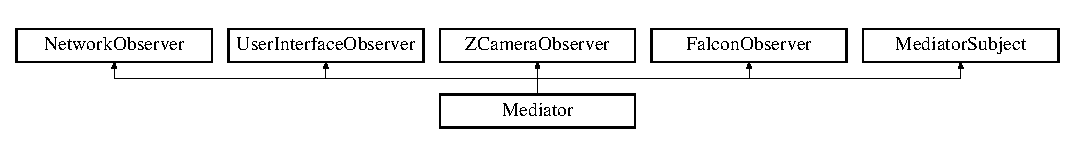
\includegraphics[height=1.49333cm]{classMediator}
\end{center}
\end{figure}
\subsection*{Public Member Functions}
\begin{DoxyCompactItemize}
\item 
\hypertarget{classMediator_abbdd9e8fbf76b85a410aec8d47591876}{
{\bfseries Mediator} (boost::shared\_\-ptr$<$ \hyperlink{classNetwork}{Network} $>$ network, boost::shared\_\-ptr$<$ \hyperlink{classFalcon}{Falcon} $>$ falcon, boost::shared\_\-ptr$<$ \hyperlink{classIZCamera}{IZCamera} $>$ zcamera, boost::shared\_\-ptr$<$ \hyperlink{classUserInterface}{UserInterface} $>$ userInterface, boost::shared\_\-ptr$<$ \hyperlink{classConfiguration}{Configuration} $>$ configuration)}
\label{classMediator_abbdd9e8fbf76b85a410aec8d47591876}

\item 
\hypertarget{classMediator_ac85a7648a8c10a5b4db08412652d668b}{
virtual void {\bfseries update} (NetworkUpdateContext context, const void $\ast$data)}
\label{classMediator_ac85a7648a8c10a5b4db08412652d668b}

\item 
\hypertarget{classMediator_ae6aa511ce52b67c8e8da9a0810db0a87}{
virtual void {\bfseries update} (UserInterfaceUpdateContext context, const void $\ast$data)}
\label{classMediator_ae6aa511ce52b67c8e8da9a0810db0a87}

\item 
\hypertarget{classMediator_a86e3c5476aac2bc9858c80aef154a6f8}{
virtual void {\bfseries update} (ZCameraUpdateContext context, const void $\ast$data)}
\label{classMediator_a86e3c5476aac2bc9858c80aef154a6f8}

\item 
\hypertarget{classMediator_a62b886c8f9e0333f70db611947579a56}{
virtual void {\bfseries update} (FalconUpdateContext context, const void $\ast$data)}
\label{classMediator_a62b886c8f9e0333f70db611947579a56}

\item 
\hypertarget{classMediator_a3d3b23d768b19d551776ce295424366a}{
virtual void {\bfseries update} (GameUpdateContext context, const void $\ast$data)}
\label{classMediator_a3d3b23d768b19d551776ce295424366a}

\end{DoxyCompactItemize}


The documentation for this class was generated from the following files:\begin{DoxyCompactItemize}
\item 
/home/kevin/workspace/HugMe/HugMe v0.9.1/Mediator/Mediator.h\item 
/home/kevin/workspace/HugMe/HugMe v0.9.1/Mediator/Mediator.cpp\end{DoxyCompactItemize}

\hypertarget{classMediatorObserver}{
\section{MediatorObserver Class Reference}
\label{classMediatorObserver}\index{MediatorObserver@{MediatorObserver}}
}


Abstract class in the observer pattern.  




{\ttfamily \#include $<$MediatorObserver.h$>$}

Inheritance diagram for MediatorObserver:\begin{figure}[H]
\begin{center}
\leavevmode
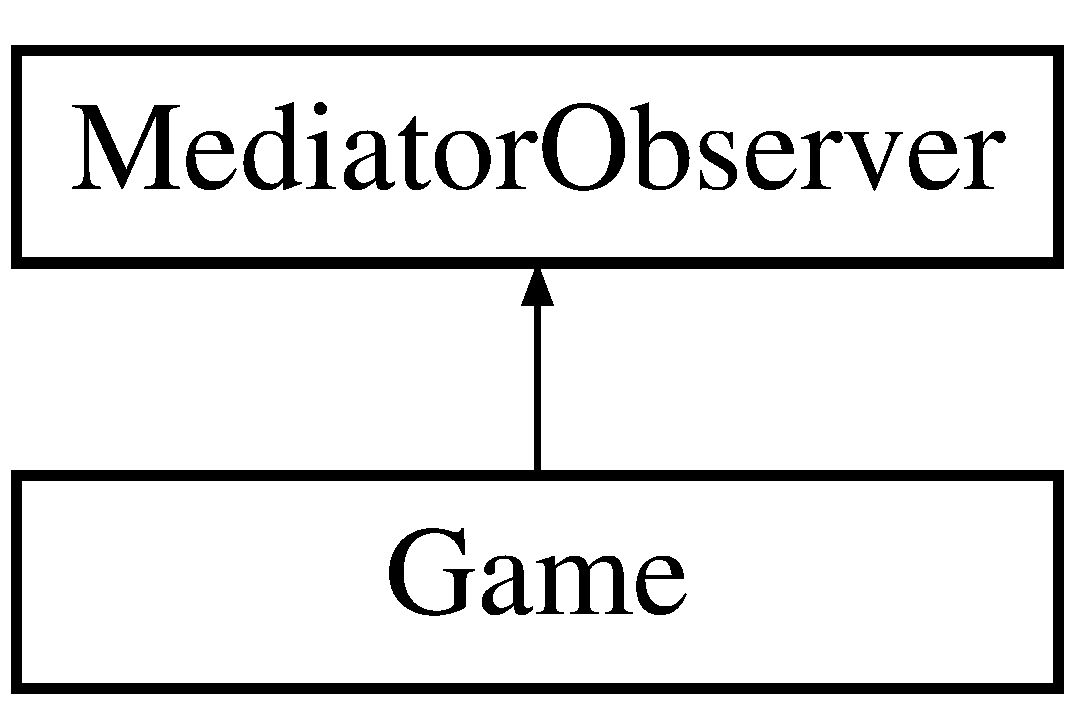
\includegraphics[height=2.000000cm]{classMediatorObserver}
\end{center}
\end{figure}
\subsection*{Public Member Functions}
\begin{DoxyCompactItemize}
\item 
\hypertarget{classMediatorObserver_afa3f47b657fb338cba632cf879396014}{
\hyperlink{classMediatorObserver_afa3f47b657fb338cba632cf879396014}{MediatorObserver} ()}
\label{classMediatorObserver_afa3f47b657fb338cba632cf879396014}

\begin{DoxyCompactList}\small\item\em Constructor. \item\end{DoxyCompactList}\item 
\hypertarget{classMediatorObserver_a62dee5cfedc7e97da55be0d2cd532f13}{
virtual \hyperlink{classMediatorObserver_a62dee5cfedc7e97da55be0d2cd532f13}{$\sim$MediatorObserver} ()}
\label{classMediatorObserver_a62dee5cfedc7e97da55be0d2cd532f13}

\begin{DoxyCompactList}\small\item\em Destructor. \item\end{DoxyCompactList}\item 
virtual void \hyperlink{classMediatorObserver_afc38ac71a1e8e0fc60fbfb4c195da44a}{update} (\hyperlink{namespaceMediatorUpdateContext_aa3a9bed543f2a2237dc2b6feea170a1d}{MediatorUpdateContext\_\-t} context, const void $\ast$data)=0
\begin{DoxyCompactList}\small\item\em Function that is called everytime the mediator has a notification to deliver. \item\end{DoxyCompactList}\end{DoxyCompactItemize}


\subsection{Detailed Description}
Abstract class in the observer pattern. The observer will receive notifications relating to user interaction with the system. 

\subsection{Member Function Documentation}
\hypertarget{classMediatorObserver_afc38ac71a1e8e0fc60fbfb4c195da44a}{
\index{MediatorObserver@{MediatorObserver}!update@{update}}
\index{update@{update}!MediatorObserver@{MediatorObserver}}
\subsubsection[{update}]{\setlength{\rightskip}{0pt plus 5cm}virtual void MediatorObserver::update (
\begin{DoxyParamCaption}
\item[{{\bf MediatorUpdateContext\_\-t}}]{ context, }
\item[{const void $\ast$}]{ data}
\end{DoxyParamCaption}
)\hspace{0.3cm}{\ttfamily  \mbox{[}pure virtual\mbox{]}}}}
\label{classMediatorObserver_afc38ac71a1e8e0fc60fbfb4c195da44a}


Function that is called everytime the mediator has a notification to deliver. 

This function should be used to handle the notifications. 

Implemented in \hyperlink{classGame_a1e83402bc85f4ef4150bee568e4f8986}{Game}.



The documentation for this class was generated from the following files:\begin{DoxyCompactItemize}
\item 
/home/kevin/workspace/HugMe/HugMe v0.9.1/Mediator/MediatorObserver.h\item 
/home/kevin/workspace/HugMe/HugMe v0.9.1/Mediator/MediatorObserver.cpp\end{DoxyCompactItemize}

\hypertarget{classMediatorSubject}{
\section{MediatorSubject Class Reference}
\label{classMediatorSubject}\index{MediatorSubject@{MediatorSubject}}
}


This class represents the mediator in the observer pattern Observers will receive notifications about various updates when the user interacts with the system.  




{\ttfamily \#include $<$MediatorSubject.h$>$}

Inheritance diagram for MediatorSubject:\begin{figure}[H]
\begin{center}
\leavevmode
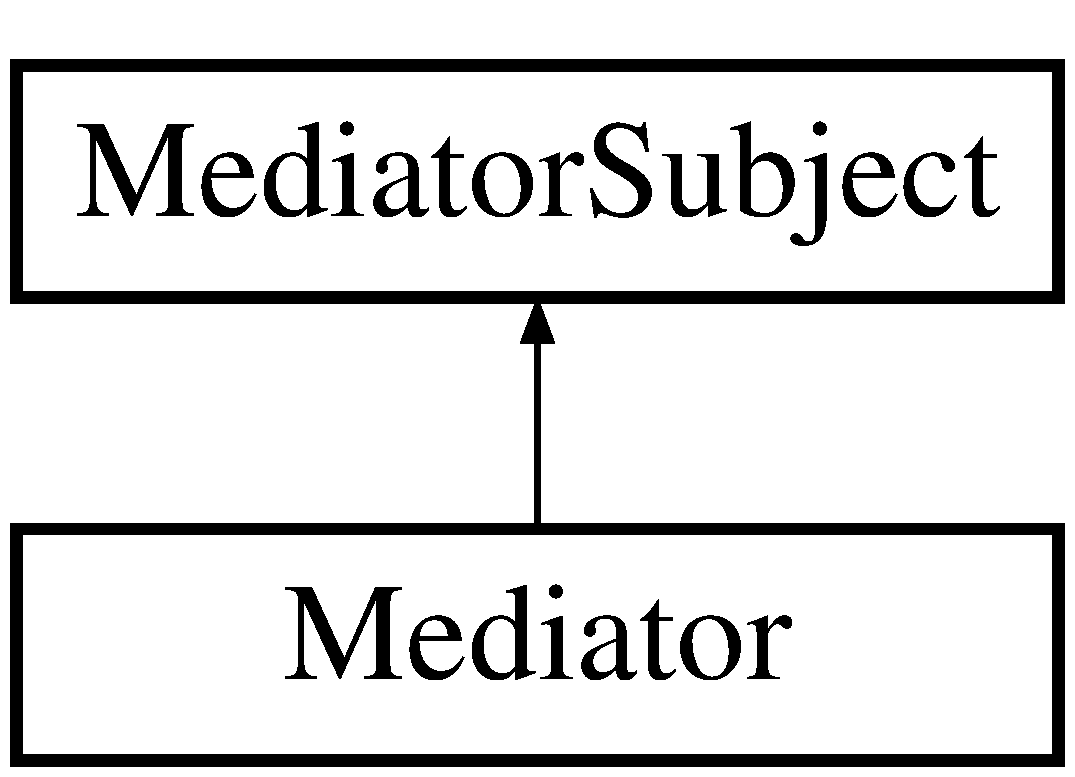
\includegraphics[height=2.000000cm]{classMediatorSubject}
\end{center}
\end{figure}
\subsection*{Public Member Functions}
\begin{DoxyCompactItemize}
\item 
\hypertarget{classMediatorSubject_a3db4b61f18f2a98025de4ab896855c27}{
\hyperlink{classMediatorSubject_a3db4b61f18f2a98025de4ab896855c27}{MediatorSubject} ()}
\label{classMediatorSubject_a3db4b61f18f2a98025de4ab896855c27}

\begin{DoxyCompactList}\small\item\em Constructor. \item\end{DoxyCompactList}\item 
\hypertarget{classMediatorSubject_a63e7e01e35bd1d073861c14a3734439b}{
virtual \hyperlink{classMediatorSubject_a63e7e01e35bd1d073861c14a3734439b}{$\sim$MediatorSubject} ()}
\label{classMediatorSubject_a63e7e01e35bd1d073861c14a3734439b}

\begin{DoxyCompactList}\small\item\em Destructor. \item\end{DoxyCompactList}\item 
\hypertarget{classMediatorSubject_aa4837dc018798cde2a754992e48e3ca0}{
void \hyperlink{classMediatorSubject_aa4837dc018798cde2a754992e48e3ca0}{attach} (\hyperlink{classMediatorObserver}{MediatorObserver} $\ast$observer)}
\label{classMediatorSubject_aa4837dc018798cde2a754992e48e3ca0}

\begin{DoxyCompactList}\small\item\em Attach an observer to this subject. \item\end{DoxyCompactList}\item 
\hypertarget{classMediatorSubject_aa3e6f03e597b315593f8ec7b654b1c23}{
void \hyperlink{classMediatorSubject_aa3e6f03e597b315593f8ec7b654b1c23}{detach} (\hyperlink{classMediatorObserver}{MediatorObserver} $\ast$observer)}
\label{classMediatorSubject_aa3e6f03e597b315593f8ec7b654b1c23}

\begin{DoxyCompactList}\small\item\em Detach an observer from this subject. \item\end{DoxyCompactList}\item 
\hypertarget{classMediatorSubject_a3bb9ea404e6bd3f3f7153cca88377049}{
void \hyperlink{classMediatorSubject_a3bb9ea404e6bd3f3f7153cca88377049}{notify} (\hyperlink{namespaceMediatorUpdateContext_aa3a9bed543f2a2237dc2b6feea170a1d}{MediatorUpdateContext\_\-t} context, const void $\ast$data=NULL)}
\label{classMediatorSubject_a3bb9ea404e6bd3f3f7153cca88377049}

\begin{DoxyCompactList}\small\item\em Notify all observers that an event happened. \item\end{DoxyCompactList}\end{DoxyCompactItemize}


\subsection{Detailed Description}
This class represents the mediator in the observer pattern Observers will receive notifications about various updates when the user interacts with the system. 

The documentation for this class was generated from the following files:\begin{DoxyCompactItemize}
\item 
/home/kevin/workspace/HugMe/HugMe v0.9.1/Mediator/MediatorSubject.h\item 
/home/kevin/workspace/HugMe/HugMe v0.9.1/Mediator/MediatorSubject.cpp\end{DoxyCompactItemize}

\hypertarget{classMFCOpenGLControl}{
\section{MFCOpenGLControl Class Reference}
\label{classMFCOpenGLControl}\index{MFCOpenGLControl@{MFCOpenGLControl}}
}
\subsection*{Public Member Functions}
\begin{DoxyCompactItemize}
\item 
\hypertarget{classMFCOpenGLControl_a3342c46d98d5f24ef1a7c7eb29ffac9f}{
void {\bfseries oglCreate} (CRect rect, CWnd $\ast$parent)}
\label{classMFCOpenGLControl_a3342c46d98d5f24ef1a7c7eb29ffac9f}

\item 
\hypertarget{classMFCOpenGLControl_a6b8a3076ae04e9872606834e90ed1e49}{
void {\bfseries oglInitialize} (void)}
\label{classMFCOpenGLControl_a6b8a3076ae04e9872606834e90ed1e49}

\item 
\hypertarget{classMFCOpenGLControl_a4055c7ec917559db7ca7a62e9ce8a7a5}{
void {\bfseries shootNewBall} (cVector3d force)}
\label{classMFCOpenGLControl_a4055c7ec917559db7ca7a62e9ce8a7a5}

\item 
\hypertarget{classMFCOpenGLControl_aa103d25f2c4867a8bf9aec0c8d4f5a08}{
void {\bfseries receiveNewBall} (cVector3d force)}
\label{classMFCOpenGLControl_aa103d25f2c4867a8bf9aec0c8d4f5a08}

\item 
\hypertarget{classMFCOpenGLControl_aaee89af6d47184edaaebda0b6d24b50e}{
UINT\_\-PTR {\bfseries startGame} (void)}
\label{classMFCOpenGLControl_aaee89af6d47184edaaebda0b6d24b50e}

\item 
\hypertarget{classMFCOpenGLControl_a01c6a55bcfbfa06d720c59c75dff33b9}{
void {\bfseries stopGame} (void)}
\label{classMFCOpenGLControl_a01c6a55bcfbfa06d720c59c75dff33b9}

\item 
\hypertarget{classMFCOpenGLControl_a297305ddb3f2572a991094ef4e1fff68}{
afx\_\-msg void {\bfseries OnPaint} ()}
\label{classMFCOpenGLControl_a297305ddb3f2572a991094ef4e1fff68}

\item 
\hypertarget{classMFCOpenGLControl_a989f49efb8a557c4d1b3b2f180dbdbdc}{
afx\_\-msg int {\bfseries OnCreate} (LPCREATESTRUCT lpCreateStruct)}
\label{classMFCOpenGLControl_a989f49efb8a557c4d1b3b2f180dbdbdc}

\item 
\hypertarget{classMFCOpenGLControl_a8956e55122f375bb9bbe4f1ad55f3470}{
afx\_\-msg void {\bfseries OnDraw} (CDC $\ast$pDC)}
\label{classMFCOpenGLControl_a8956e55122f375bb9bbe4f1ad55f3470}

\item 
\hypertarget{classMFCOpenGLControl_a6b585bc2fa6380208b8e9af5d91ceddf}{
afx\_\-msg void {\bfseries OnSize} (UINT nType, int cx, int cy)}
\label{classMFCOpenGLControl_a6b585bc2fa6380208b8e9af5d91ceddf}

\item 
\hypertarget{classMFCOpenGLControl_ace04284c25e46ca408a05cf4f2a9ccd4}{
afx\_\-msg void {\bfseries OnTimer} (UINT\_\-PTR nIDEvent)}
\label{classMFCOpenGLControl_ace04284c25e46ca408a05cf4f2a9ccd4}

\end{DoxyCompactItemize}
\subsection*{Data Fields}
\begin{DoxyCompactItemize}
\item 
\hypertarget{classMFCOpenGLControl_a3c140c9546324bc1547a7a309ad71aed}{
UINT\_\-PTR {\bfseries m\_\-unpTimer}}
\label{classMFCOpenGLControl_a3c140c9546324bc1547a7a309ad71aed}

\end{DoxyCompactItemize}


The documentation for this class was generated from the following files:\begin{DoxyCompactItemize}
\item 
/home/kevin/workspace/HugMe/HugMe v0.9.1/UserInterface/MFCOpenGLControl.h\item 
/home/kevin/workspace/HugMe/HugMe v0.9.1/UserInterface/MFCOpenGLControl.cpp\end{DoxyCompactItemize}

\hypertarget{classMFCUserInterface}{
\section{MFCUserInterface Class Reference}
\label{classMFCUserInterface}\index{MFCUserInterface@{MFCUserInterface}}
}
Inheritance diagram for MFCUserInterface:\begin{figure}[H]
\begin{center}
\leavevmode
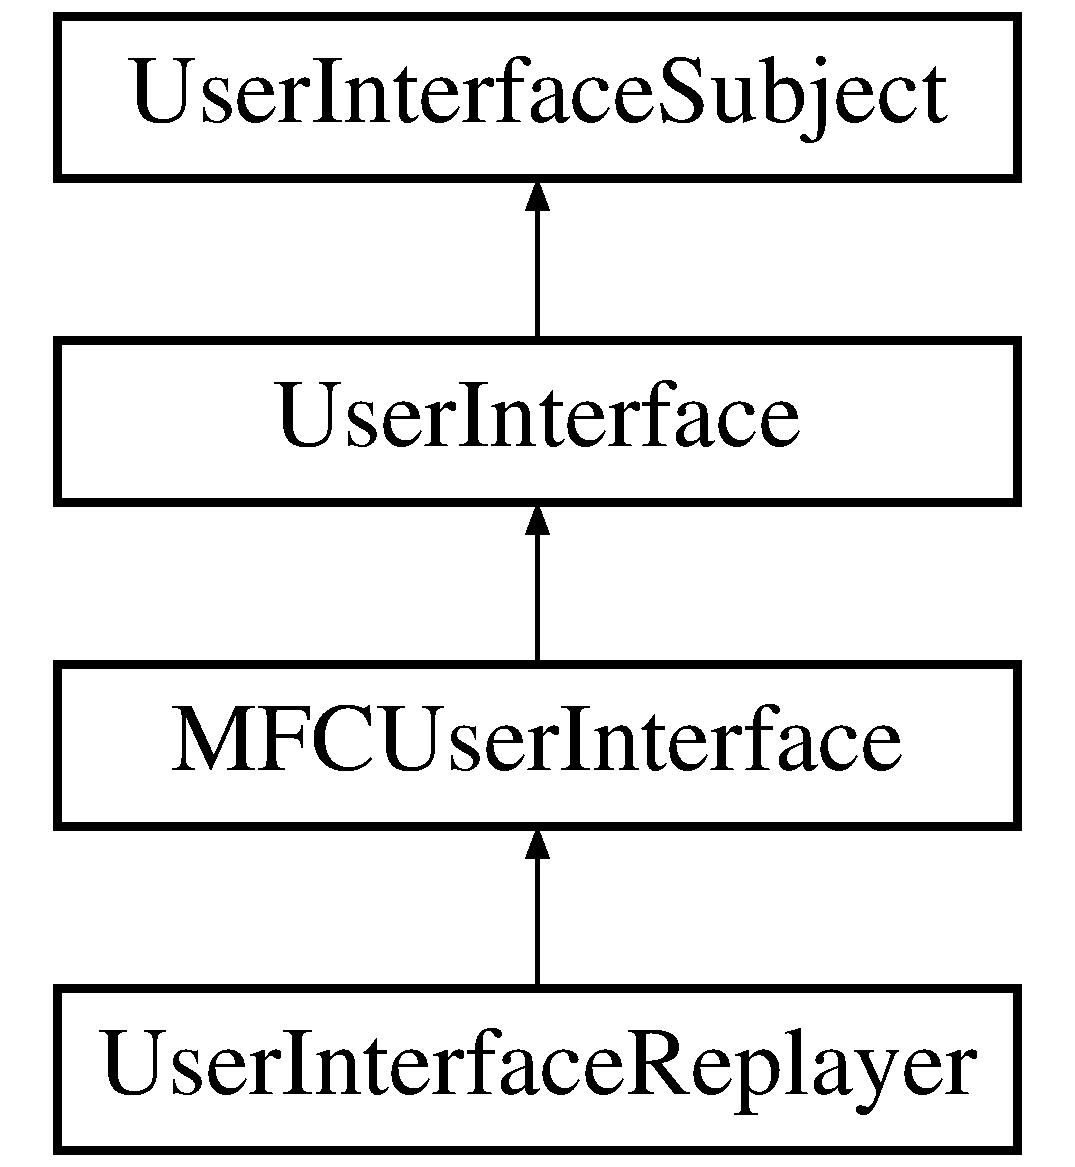
\includegraphics[height=4cm]{classMFCUserInterface}
\end{center}
\end{figure}
\subsection*{Public Member Functions}
\begin{DoxyCompactItemize}
\item 
\hypertarget{classMFCUserInterface_a7ac72f8cddb94419db9c9ed261ace1b1}{
{\bfseries MFCUserInterface} (const \hyperlink{structUserPreferences}{UserPreferences} \&preferences)}
\label{classMFCUserInterface_a7ac72f8cddb94419db9c9ed261ace1b1}

\item 
\hypertarget{classMFCUserInterface_affc39ae32cd234575ce95db40701db01}{
virtual void {\bfseries displayConnectionStateChanged} (ConnectionState\_\-t state, Player\_\-t player)}
\label{classMFCUserInterface_affc39ae32cd234575ce95db40701db01}

\item 
\hypertarget{classMFCUserInterface_a5cf1751505da89dc55df1fb12318bd96}{
virtual void {\bfseries displayGameStateChanged} (GameState\_\-t state, Player\_\-t player)}
\label{classMFCUserInterface_a5cf1751505da89dc55df1fb12318bd96}

\item 
\hypertarget{classMFCUserInterface_a1eb12e6f9b8729361008d9abd290d245}{
virtual void {\bfseries displayConnectionFailed} ()}
\label{classMFCUserInterface_a1eb12e6f9b8729361008d9abd290d245}

\item 
\hypertarget{classMFCUserInterface_a1ad6e96350df96d07b0f4de186c1677c}{
virtual void {\bfseries displayFailedToListen} ()}
\label{classMFCUserInterface_a1ad6e96350df96d07b0f4de186c1677c}

\item 
\hypertarget{classMFCUserInterface_a12aafbe2449d1eff42150b84e2b403b2}{
virtual void {\bfseries displayNetworkError} ()}
\label{classMFCUserInterface_a12aafbe2449d1eff42150b84e2b403b2}

\item 
\hypertarget{classMFCUserInterface_a211917cb2e10228e4cabd54d5b411106}{
virtual void {\bfseries displayPeerChatMessage} (const std::string \&message)}
\label{classMFCUserInterface_a211917cb2e10228e4cabd54d5b411106}

\item 
\hypertarget{classMFCUserInterface_a93930bcf41087f4f1c0380f12b190714}{
virtual void {\bfseries displayLocalFrame} (const \hyperlink{structVideoData}{VideoData} \&video)}
\label{classMFCUserInterface_a93930bcf41087f4f1c0380f12b190714}

\item 
\hypertarget{classMFCUserInterface_afea24df787ef3ebdd57ad7c6435e14cc}{
virtual void {\bfseries displayRemoteFrame} (const \hyperlink{structVideoData}{VideoData} \&video)}
\label{classMFCUserInterface_afea24df787ef3ebdd57ad7c6435e14cc}

\item 
\hypertarget{classMFCUserInterface_a25bf67955e01502250d4239ea6dc9e6d}{
virtual void {\bfseries networkConnectButtonPushed} ()}
\label{classMFCUserInterface_a25bf67955e01502250d4239ea6dc9e6d}

\item 
\hypertarget{classMFCUserInterface_ad19ff1d9fe21137d564c7f91d6d9638a}{
virtual void {\bfseries networkListenButtonPushed} ()}
\label{classMFCUserInterface_ad19ff1d9fe21137d564c7f91d6d9638a}

\item 
\hypertarget{classMFCUserInterface_a05124c9a819899bf74dbbbd1ba27d32d}{
virtual void {\bfseries networkDisconnectButtonPushed} ()}
\label{classMFCUserInterface_a05124c9a819899bf74dbbbd1ba27d32d}

\item 
\hypertarget{classMFCUserInterface_a645879dc2e81a2d2810d215bbc435d87}{
virtual void {\bfseries sendChatButtonPushed} (const std::string \&message)}
\label{classMFCUserInterface_a645879dc2e81a2d2810d215bbc435d87}

\item 
\hypertarget{classMFCUserInterface_a3ded83efa5ecbc38a21051dd90dc661e}{
virtual void {\bfseries startGameButtonPushed} ()}
\label{classMFCUserInterface_a3ded83efa5ecbc38a21051dd90dc661e}

\item 
\hypertarget{classMFCUserInterface_a0bfd2943d3cf9e704bb71880eb3aa865}{
virtual void {\bfseries exitGameButtonPushed} ()}
\label{classMFCUserInterface_a0bfd2943d3cf9e704bb71880eb3aa865}

\item 
\hypertarget{classMFCUserInterface_a99a9356281a3d713e0fda41940f7a6fb}{
virtual void {\bfseries pauseGameButtonPushed} ()}
\label{classMFCUserInterface_a99a9356281a3d713e0fda41940f7a6fb}

\item 
\hypertarget{classMFCUserInterface_ab979a02b0fb024ebdd2e8cc958e26d42}{
virtual void {\bfseries changePreferences} (const \hyperlink{structUserPreferences}{UserPreferences} \&preferences)}
\label{classMFCUserInterface_ab979a02b0fb024ebdd2e8cc958e26d42}

\item 
\hypertarget{classMFCUserInterface_a0953b5a6a8880539f48e33828e1ebdac}{
virtual void {\bfseries closeApplication} ()}
\label{classMFCUserInterface_a0953b5a6a8880539f48e33828e1ebdac}

\item 
\hypertarget{classMFCUserInterface_a37ad511facfb8e5b6f34059a3ebf9f57}{
virtual void {\bfseries setPeerUserName} (const std::string \&name)}
\label{classMFCUserInterface_a37ad511facfb8e5b6f34059a3ebf9f57}

\item 
\hypertarget{classMFCUserInterface_afbd06e08b7e16ff1df6df06cdd3429e5}{
virtual void {\bfseries notifyNewBallShot} (const cVector3d \&force)}
\label{classMFCUserInterface_afbd06e08b7e16ff1df6df06cdd3429e5}

\item 
\hypertarget{classMFCUserInterface_aa592d72e4c2e6e482f363ce69b46250f}{
virtual void {\bfseries receiveNewBall} (const cVector3d \&force)}
\label{classMFCUserInterface_aa592d72e4c2e6e482f363ce69b46250f}

\item 
\hypertarget{classMFCUserInterface_a03a72e69e2586b52ba3acac1e6b39700}{
CDialog $\ast$ {\bfseries getMainWindow} ()}
\label{classMFCUserInterface_a03a72e69e2586b52ba3acac1e6b39700}

\end{DoxyCompactItemize}
\subsection*{Protected Attributes}
\begin{DoxyCompactItemize}
\item 
\hypertarget{classMFCUserInterface_a548760ec3e8f659b262ef3aab3709e7f}{
\hyperlink{classCMainDlg}{CMainDlg} $\ast$ {\bfseries m\_\-pMainDlg}}
\label{classMFCUserInterface_a548760ec3e8f659b262ef3aab3709e7f}

\end{DoxyCompactItemize}


The documentation for this class was generated from the following files:\begin{DoxyCompactItemize}
\item 
/home/kevin/workspace/HugMe/HugMe v0.9.1/UserInterface/MFCUserInterface.h\item 
/home/kevin/workspace/HugMe/HugMe v0.9.1/UserInterface/MFCUserInterface.cpp\end{DoxyCompactItemize}

\hypertarget{classNetwork}{
\section{Network Class Reference}
\label{classNetwork}\index{Network@{Network}}
}


Abstract class representing the networking component of the application all network interfaces should be able to send and receive data.  




{\ttfamily \#include $<$Network.h$>$}

Inheritance diagram for Network:\begin{figure}[H]
\begin{center}
\leavevmode
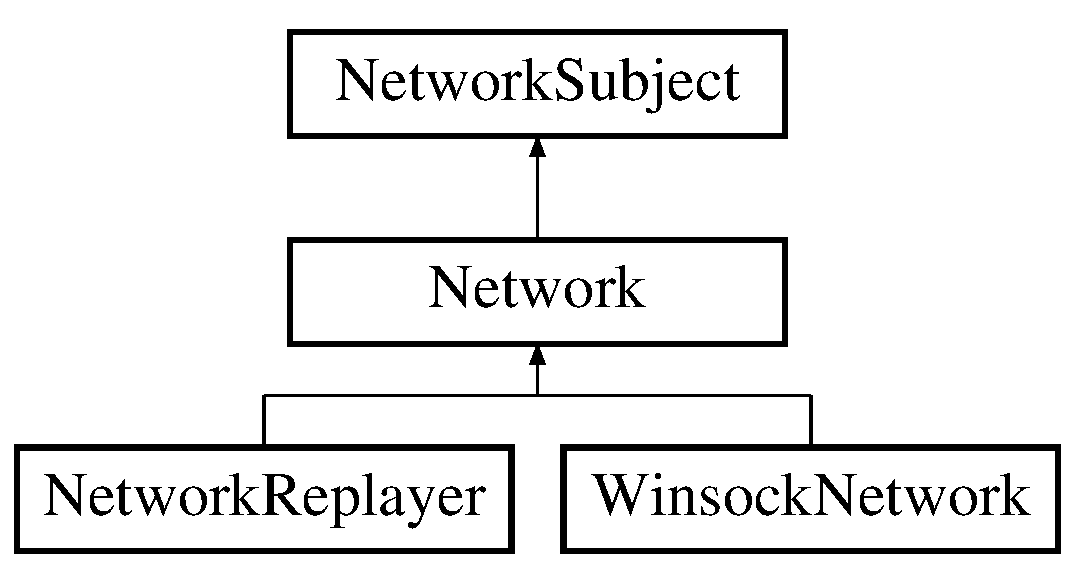
\includegraphics[height=3.000000cm]{classNetwork}
\end{center}
\end{figure}
\subsection*{Public Member Functions}
\begin{DoxyCompactItemize}
\item 
\hypertarget{classNetwork_a3cc2fb4f8fa4d507077e8da85ce5a1c8}{
\hyperlink{classNetwork_a3cc2fb4f8fa4d507077e8da85ce5a1c8}{Network} ()}
\label{classNetwork_a3cc2fb4f8fa4d507077e8da85ce5a1c8}

\begin{DoxyCompactList}\small\item\em Constructor. \item\end{DoxyCompactList}\item 
\hypertarget{classNetwork_a7a4e19cdb4bf0c7ecf82baa643831492}{
virtual \hyperlink{classNetwork_a7a4e19cdb4bf0c7ecf82baa643831492}{$\sim$Network} ()}
\label{classNetwork_a7a4e19cdb4bf0c7ecf82baa643831492}

\begin{DoxyCompactList}\small\item\em Destructor. \item\end{DoxyCompactList}\item 
virtual rc\_\-network \hyperlink{classNetwork_afb5306e2b769c01780aaa44d2c14306d}{listen} (const std::string \&userName)=0
\begin{DoxyCompactList}\small\item\em Start listening for connections. \item\end{DoxyCompactList}\item 
virtual rc\_\-network \hyperlink{classNetwork_a105f5e229e0ac9ff2b718dd34112c292}{connect} (const std::string \&ipAddress, const std::string \&userName)=0
\begin{DoxyCompactList}\small\item\em Attempt to connect to a peer. \item\end{DoxyCompactList}\item 
virtual rc\_\-network \hyperlink{classNetwork_a1b0e29fc9936615e76c1db95caba0a9e}{disconnect} ()=0
\begin{DoxyCompactList}\small\item\em Disconnect from a peer. \item\end{DoxyCompactList}\item 
virtual rc\_\-network \hyperlink{classNetwork_a3f6b451fd546f2e44eb2c14661bc1ad3}{sendStartGame} ()=0
\begin{DoxyCompactList}\small\item\em Send a start game message to the peer. \item\end{DoxyCompactList}\item 
virtual rc\_\-network \hyperlink{classNetwork_ac60291a8d99468ebc38d085fc0455df0}{sendPauseGame} ()=0
\begin{DoxyCompactList}\small\item\em Send a pause game message to the peer. \item\end{DoxyCompactList}\item 
virtual rc\_\-network \hyperlink{classNetwork_ae3f72f3003309c6d38105f504db8ce05}{sendEndGame} ()=0
\begin{DoxyCompactList}\small\item\em Send an end game message to the peer. \item\end{DoxyCompactList}\item 
virtual rc\_\-network \hyperlink{classNetwork_a741e75b2e9adfc188c53e150b4dd4610}{sendUserName} (const std::string \&userName)=0
\begin{DoxyCompactList}\small\item\em Send our username to the peer. \item\end{DoxyCompactList}\item 
virtual rc\_\-network \hyperlink{classNetwork_aa5e1e44e3cb4862b2c343999c89ce3b5}{sendChatMessage} (const std::string \&message)=0
\begin{DoxyCompactList}\small\item\em Send a chat message to the peer. \item\end{DoxyCompactList}\item 
virtual rc\_\-network \hyperlink{classNetwork_a189df8819d21d4f1a277ca753453045b}{sendVideoData} (const \hyperlink{structVideoData}{VideoData} \&video)=0
\begin{DoxyCompactList}\small\item\em Send video data to the peer. \item\end{DoxyCompactList}\item 
virtual rc\_\-network \hyperlink{classNetwork_a9a2eb94c34d8d93f7490184cd2526e62}{sendPlayerPosition} (const cVector3d \&position)=0
\begin{DoxyCompactList}\small\item\em Send the players position to the peer. \item\end{DoxyCompactList}\item 
virtual rc\_\-network \hyperlink{classNetwork_aa105332ed8a1325a89f1f3e0a9d27521}{sendSlingshotPosition} (const cVector3d \&position)=0
\begin{DoxyCompactList}\small\item\em Send the slingshot position to the peer. \item\end{DoxyCompactList}\item 
virtual rc\_\-network \hyperlink{classNetwork_a477324500341f146fc7fc7411290a424}{sendProjectile} (const \hyperlink{classProjectile}{Projectile} \&projectile)=0
\begin{DoxyCompactList}\small\item\em Send a projectile to the peer. \item\end{DoxyCompactList}\item 
virtual rc\_\-network \hyperlink{classNetwork_ad4fd766e5bae5a3f002a26218b60b426}{sendSlingshotPullback} ()=0
\begin{DoxyCompactList}\small\item\em Send a slingshot pullback event to the peer. \item\end{DoxyCompactList}\item 
virtual bool \hyperlink{classNetwork_ab84ebbf03390c5ee99a27e2b340e3518}{isConnected} () const =0
\begin{DoxyCompactList}\small\item\em Determines if we are connected to a peer. \item\end{DoxyCompactList}\item 
virtual bool \hyperlink{classNetwork_a1e8342d061f8e1b28d50d966e946650b}{isListening} () const =0
\begin{DoxyCompactList}\small\item\em Determines if we are listening for connections. \item\end{DoxyCompactList}\end{DoxyCompactItemize}


\subsection{Detailed Description}
Abstract class representing the networking component of the application all network interfaces should be able to send and receive data. 

\subsection{Member Function Documentation}
\hypertarget{classNetwork_a105f5e229e0ac9ff2b718dd34112c292}{
\index{Network@{Network}!connect@{connect}}
\index{connect@{connect}!Network@{Network}}
\subsubsection[{connect}]{\setlength{\rightskip}{0pt plus 5cm}virtual rc\_\-network Network::connect (
\begin{DoxyParamCaption}
\item[{const std::string \&}]{ ipAddress, }
\item[{const std::string \&}]{ userName}
\end{DoxyParamCaption}
)\hspace{0.3cm}{\ttfamily  \mbox{[}pure virtual\mbox{]}}}}
\label{classNetwork_a105f5e229e0ac9ff2b718dd34112c292}


Attempt to connect to a peer. 


\begin{DoxyParams}{Parameters}
\item[{\em ipAddress}]The ip address that we will connect to \item[{\em userName}]The username that will be used to establish the connection \end{DoxyParams}
\begin{DoxyReturn}{Returns}
The error code, SUCCESS if we are now connected to the peer 
\end{DoxyReturn}


Implemented in \hyperlink{classWinsockNetwork_a0f7f289635183b1082894f230a989006}{WinsockNetwork}, and \hyperlink{classNetworkReplayer_a6d4deeeede0cd5c07b44489a33c113f5}{NetworkReplayer}.

\hypertarget{classNetwork_a1b0e29fc9936615e76c1db95caba0a9e}{
\index{Network@{Network}!disconnect@{disconnect}}
\index{disconnect@{disconnect}!Network@{Network}}
\subsubsection[{disconnect}]{\setlength{\rightskip}{0pt plus 5cm}virtual rc\_\-network Network::disconnect (
\begin{DoxyParamCaption}
{}
\end{DoxyParamCaption}
)\hspace{0.3cm}{\ttfamily  \mbox{[}pure virtual\mbox{]}}}}
\label{classNetwork_a1b0e29fc9936615e76c1db95caba0a9e}


Disconnect from a peer. 

\begin{DoxyReturn}{Returns}
The error code, SUCCESS if we successfully disconnected 
\end{DoxyReturn}


Implemented in \hyperlink{classWinsockNetwork_abd947a2edb4d5053286f25b4c9f041c1}{WinsockNetwork}, and \hyperlink{classNetworkReplayer_a3aab774a33a87446aa874871fea54655}{NetworkReplayer}.

\hypertarget{classNetwork_ab84ebbf03390c5ee99a27e2b340e3518}{
\index{Network@{Network}!isConnected@{isConnected}}
\index{isConnected@{isConnected}!Network@{Network}}
\subsubsection[{isConnected}]{\setlength{\rightskip}{0pt plus 5cm}virtual bool Network::isConnected (
\begin{DoxyParamCaption}
{}
\end{DoxyParamCaption}
) const\hspace{0.3cm}{\ttfamily  \mbox{[}pure virtual\mbox{]}}}}
\label{classNetwork_ab84ebbf03390c5ee99a27e2b340e3518}


Determines if we are connected to a peer. 

\begin{DoxyReturn}{Returns}
true if we are connected to a peer 
\end{DoxyReturn}


Implemented in \hyperlink{classWinsockNetwork_a8c621566b7ce641d86797569346fcaad}{WinsockNetwork}, and \hyperlink{classNetworkReplayer_a3656c06c32e76a30ac48055a0695d99a}{NetworkReplayer}.

\hypertarget{classNetwork_a1e8342d061f8e1b28d50d966e946650b}{
\index{Network@{Network}!isListening@{isListening}}
\index{isListening@{isListening}!Network@{Network}}
\subsubsection[{isListening}]{\setlength{\rightskip}{0pt plus 5cm}virtual bool Network::isListening (
\begin{DoxyParamCaption}
{}
\end{DoxyParamCaption}
) const\hspace{0.3cm}{\ttfamily  \mbox{[}pure virtual\mbox{]}}}}
\label{classNetwork_a1e8342d061f8e1b28d50d966e946650b}


Determines if we are listening for connections. 

\begin{DoxyReturn}{Returns}
true if we are listening for connections 
\end{DoxyReturn}


Implemented in \hyperlink{classWinsockNetwork_a7cbc0e15323359b9bdb862342e406f23}{WinsockNetwork}, and \hyperlink{classNetworkReplayer_a869c34b845f18eb262ead68542662aa4}{NetworkReplayer}.

\hypertarget{classNetwork_afb5306e2b769c01780aaa44d2c14306d}{
\index{Network@{Network}!listen@{listen}}
\index{listen@{listen}!Network@{Network}}
\subsubsection[{listen}]{\setlength{\rightskip}{0pt plus 5cm}virtual rc\_\-network Network::listen (
\begin{DoxyParamCaption}
\item[{const std::string \&}]{ userName}
\end{DoxyParamCaption}
)\hspace{0.3cm}{\ttfamily  \mbox{[}pure virtual\mbox{]}}}}
\label{classNetwork_afb5306e2b769c01780aaa44d2c14306d}


Start listening for connections. 


\begin{DoxyParams}{Parameters}
\item[{\em userName}]The username used to establish the connection \end{DoxyParams}
\begin{DoxyReturn}{Returns}
The error code, SUCCESS if listening was successful 
\end{DoxyReturn}


Implemented in \hyperlink{classWinsockNetwork_a6f2f806a0e246a46ff6d0c2006cddd43}{WinsockNetwork}, and \hyperlink{classNetworkReplayer_a54f644fe92941370481c45989bad6615}{NetworkReplayer}.

\hypertarget{classNetwork_aa5e1e44e3cb4862b2c343999c89ce3b5}{
\index{Network@{Network}!sendChatMessage@{sendChatMessage}}
\index{sendChatMessage@{sendChatMessage}!Network@{Network}}
\subsubsection[{sendChatMessage}]{\setlength{\rightskip}{0pt plus 5cm}virtual rc\_\-network Network::sendChatMessage (
\begin{DoxyParamCaption}
\item[{const std::string \&}]{ message}
\end{DoxyParamCaption}
)\hspace{0.3cm}{\ttfamily  \mbox{[}pure virtual\mbox{]}}}}
\label{classNetwork_aa5e1e44e3cb4862b2c343999c89ce3b5}


Send a chat message to the peer. 


\begin{DoxyParams}{Parameters}
\item[{\em message}]The chat message that will be sent to the peer. \end{DoxyParams}
\begin{DoxyReturn}{Returns}
The error code, SUCCESS if the message was sent and received 
\end{DoxyReturn}


Implemented in \hyperlink{classWinsockNetwork_a420d4e6b5c698476a94dcdb503233de7}{WinsockNetwork}, and \hyperlink{classNetworkReplayer_a689bc26f935bb0d7f72d3f69cea6e98c}{NetworkReplayer}.

\hypertarget{classNetwork_ae3f72f3003309c6d38105f504db8ce05}{
\index{Network@{Network}!sendEndGame@{sendEndGame}}
\index{sendEndGame@{sendEndGame}!Network@{Network}}
\subsubsection[{sendEndGame}]{\setlength{\rightskip}{0pt plus 5cm}virtual rc\_\-network Network::sendEndGame (
\begin{DoxyParamCaption}
{}
\end{DoxyParamCaption}
)\hspace{0.3cm}{\ttfamily  \mbox{[}pure virtual\mbox{]}}}}
\label{classNetwork_ae3f72f3003309c6d38105f504db8ce05}


Send an end game message to the peer. 

\begin{DoxyReturn}{Returns}
The error code, SUCCESS if the message was sent and received 
\end{DoxyReturn}


Implemented in \hyperlink{classWinsockNetwork_a877c8001bbd880295e0458c3377dca25}{WinsockNetwork}, and \hyperlink{classNetworkReplayer_a33c840b356485101092fe220d4aa73fb}{NetworkReplayer}.

\hypertarget{classNetwork_ac60291a8d99468ebc38d085fc0455df0}{
\index{Network@{Network}!sendPauseGame@{sendPauseGame}}
\index{sendPauseGame@{sendPauseGame}!Network@{Network}}
\subsubsection[{sendPauseGame}]{\setlength{\rightskip}{0pt plus 5cm}virtual rc\_\-network Network::sendPauseGame (
\begin{DoxyParamCaption}
{}
\end{DoxyParamCaption}
)\hspace{0.3cm}{\ttfamily  \mbox{[}pure virtual\mbox{]}}}}
\label{classNetwork_ac60291a8d99468ebc38d085fc0455df0}


Send a pause game message to the peer. 

\begin{DoxyReturn}{Returns}
The error code, SUCCESS if the message was sent and received 
\end{DoxyReturn}


Implemented in \hyperlink{classWinsockNetwork_ae4412629d2ee052afc41c81f36cfad50}{WinsockNetwork}, and \hyperlink{classNetworkReplayer_aa54ba87a728ebdb0f23a82e409094468}{NetworkReplayer}.

\hypertarget{classNetwork_a9a2eb94c34d8d93f7490184cd2526e62}{
\index{Network@{Network}!sendPlayerPosition@{sendPlayerPosition}}
\index{sendPlayerPosition@{sendPlayerPosition}!Network@{Network}}
\subsubsection[{sendPlayerPosition}]{\setlength{\rightskip}{0pt plus 5cm}virtual rc\_\-network Network::sendPlayerPosition (
\begin{DoxyParamCaption}
\item[{const cVector3d \&}]{ position}
\end{DoxyParamCaption}
)\hspace{0.3cm}{\ttfamily  \mbox{[}pure virtual\mbox{]}}}}
\label{classNetwork_a9a2eb94c34d8d93f7490184cd2526e62}


Send the players position to the peer. 


\begin{DoxyParams}{Parameters}
\item[{\em position}]Our player position that will be sent to the peer. \end{DoxyParams}
\begin{DoxyReturn}{Returns}
The error code, SUCCESS if the message was sent and received 
\end{DoxyReturn}


Implemented in \hyperlink{classWinsockNetwork_ab27dd7393a89573f9e75e1a50efbc833}{WinsockNetwork}, and \hyperlink{classNetworkReplayer_a7c9a5203b80840fee0157d506ff14f61}{NetworkReplayer}.

\hypertarget{classNetwork_a477324500341f146fc7fc7411290a424}{
\index{Network@{Network}!sendProjectile@{sendProjectile}}
\index{sendProjectile@{sendProjectile}!Network@{Network}}
\subsubsection[{sendProjectile}]{\setlength{\rightskip}{0pt plus 5cm}virtual rc\_\-network Network::sendProjectile (
\begin{DoxyParamCaption}
\item[{const {\bf Projectile} \&}]{ projectile}
\end{DoxyParamCaption}
)\hspace{0.3cm}{\ttfamily  \mbox{[}pure virtual\mbox{]}}}}
\label{classNetwork_a477324500341f146fc7fc7411290a424}


Send a projectile to the peer. 


\begin{DoxyParams}{Parameters}
\item[{\em projectile}]The projectile that will be sent to the peer. \end{DoxyParams}
\begin{DoxyReturn}{Returns}
The error code, SUCCESS if the message was sent and received 
\end{DoxyReturn}


Implemented in \hyperlink{classWinsockNetwork_accb610c314dd94a1649bcfe101c93997}{WinsockNetwork}, and \hyperlink{classNetworkReplayer_a7ebdbb74bb8e3b1fdc877d3c8157d342}{NetworkReplayer}.

\hypertarget{classNetwork_aa105332ed8a1325a89f1f3e0a9d27521}{
\index{Network@{Network}!sendSlingshotPosition@{sendSlingshotPosition}}
\index{sendSlingshotPosition@{sendSlingshotPosition}!Network@{Network}}
\subsubsection[{sendSlingshotPosition}]{\setlength{\rightskip}{0pt plus 5cm}virtual rc\_\-network Network::sendSlingshotPosition (
\begin{DoxyParamCaption}
\item[{const cVector3d \&}]{ position}
\end{DoxyParamCaption}
)\hspace{0.3cm}{\ttfamily  \mbox{[}pure virtual\mbox{]}}}}
\label{classNetwork_aa105332ed8a1325a89f1f3e0a9d27521}


Send the slingshot position to the peer. 


\begin{DoxyParams}{Parameters}
\item[{\em position}]Our slingshot position that will be sent to the peer. \end{DoxyParams}
\begin{DoxyReturn}{Returns}
The error code, SUCCESS if the message was sent and received 
\end{DoxyReturn}


Implemented in \hyperlink{classWinsockNetwork_af0456294cf39244cc59f1ca81e2aa2d3}{WinsockNetwork}, and \hyperlink{classNetworkReplayer_ad8ad840c17aa86b890857ef714eb019a}{NetworkReplayer}.

\hypertarget{classNetwork_ad4fd766e5bae5a3f002a26218b60b426}{
\index{Network@{Network}!sendSlingshotPullback@{sendSlingshotPullback}}
\index{sendSlingshotPullback@{sendSlingshotPullback}!Network@{Network}}
\subsubsection[{sendSlingshotPullback}]{\setlength{\rightskip}{0pt plus 5cm}virtual rc\_\-network Network::sendSlingshotPullback (
\begin{DoxyParamCaption}
{}
\end{DoxyParamCaption}
)\hspace{0.3cm}{\ttfamily  \mbox{[}pure virtual\mbox{]}}}}
\label{classNetwork_ad4fd766e5bae5a3f002a26218b60b426}


Send a slingshot pullback event to the peer. 

This lets the peer know that we have started to pull back our slingshot. \begin{DoxyReturn}{Returns}
The error code, SUCCESS if the message was sent and received 
\end{DoxyReturn}


Implemented in \hyperlink{classWinsockNetwork_a0a8ced3a30f215e71114b9fa94b3d1e3}{WinsockNetwork}, and \hyperlink{classNetworkReplayer_a98342ea3e802e9108b6d3329d977eade}{NetworkReplayer}.

\hypertarget{classNetwork_a3f6b451fd546f2e44eb2c14661bc1ad3}{
\index{Network@{Network}!sendStartGame@{sendStartGame}}
\index{sendStartGame@{sendStartGame}!Network@{Network}}
\subsubsection[{sendStartGame}]{\setlength{\rightskip}{0pt plus 5cm}virtual rc\_\-network Network::sendStartGame (
\begin{DoxyParamCaption}
{}
\end{DoxyParamCaption}
)\hspace{0.3cm}{\ttfamily  \mbox{[}pure virtual\mbox{]}}}}
\label{classNetwork_a3f6b451fd546f2e44eb2c14661bc1ad3}


Send a start game message to the peer. 

\begin{DoxyReturn}{Returns}
The error code, SUCCESS if the message was sent and received 
\end{DoxyReturn}


Implemented in \hyperlink{classWinsockNetwork_a20ed4411ec34336c6a213b15cc3fcad9}{WinsockNetwork}, and \hyperlink{classNetworkReplayer_aa9f70d4eee3d630c36c2bbc71bb7e195}{NetworkReplayer}.

\hypertarget{classNetwork_a741e75b2e9adfc188c53e150b4dd4610}{
\index{Network@{Network}!sendUserName@{sendUserName}}
\index{sendUserName@{sendUserName}!Network@{Network}}
\subsubsection[{sendUserName}]{\setlength{\rightskip}{0pt plus 5cm}virtual rc\_\-network Network::sendUserName (
\begin{DoxyParamCaption}
\item[{const std::string \&}]{ userName}
\end{DoxyParamCaption}
)\hspace{0.3cm}{\ttfamily  \mbox{[}pure virtual\mbox{]}}}}
\label{classNetwork_a741e75b2e9adfc188c53e150b4dd4610}


Send our username to the peer. 

The user name is sent when the connection is established so this should only be used if a user changes there username 
\begin{DoxyParams}{Parameters}
\item[{\em userName}]Our new username that will be sent to the peer \end{DoxyParams}
\begin{DoxyReturn}{Returns}
The error code, SUCCESS if the message was sent and received 
\end{DoxyReturn}


Implemented in \hyperlink{classWinsockNetwork_ae76b6c306ef15d162fe652c38c78d4e2}{WinsockNetwork}, and \hyperlink{classNetworkReplayer_a49bb75f65853c34c0bdafa6aba066056}{NetworkReplayer}.

\hypertarget{classNetwork_a189df8819d21d4f1a277ca753453045b}{
\index{Network@{Network}!sendVideoData@{sendVideoData}}
\index{sendVideoData@{sendVideoData}!Network@{Network}}
\subsubsection[{sendVideoData}]{\setlength{\rightskip}{0pt plus 5cm}virtual rc\_\-network Network::sendVideoData (
\begin{DoxyParamCaption}
\item[{const {\bf VideoData} \&}]{ video}
\end{DoxyParamCaption}
)\hspace{0.3cm}{\ttfamily  \mbox{[}pure virtual\mbox{]}}}}
\label{classNetwork_a189df8819d21d4f1a277ca753453045b}


Send video data to the peer. 


\begin{DoxyParams}{Parameters}
\item[{\em video}]The video data that will be sent to the peer. \end{DoxyParams}
\begin{DoxyReturn}{Returns}
The error code, SUCCESS if the message was sent and received 
\end{DoxyReturn}


Implemented in \hyperlink{classWinsockNetwork_a36362dbaa70fbe00dd48fded21464888}{WinsockNetwork}, and \hyperlink{classNetworkReplayer_ab7f69701316a3387da91d2146ea97b5e}{NetworkReplayer}.



The documentation for this class was generated from the following files:\begin{DoxyCompactItemize}
\item 
/home/kevin/workspace/HugMe/HugMe v0.9.1/Network/Network.h\item 
/home/kevin/workspace/HugMe/HugMe v0.9.1/Network/Network.cpp\end{DoxyCompactItemize}

\hypertarget{classNetworkObserver}{
\section{NetworkObserver Class Reference}
\label{classNetworkObserver}\index{NetworkObserver@{NetworkObserver}}
}
Inheritance diagram for NetworkObserver:\begin{figure}[H]
\begin{center}
\leavevmode
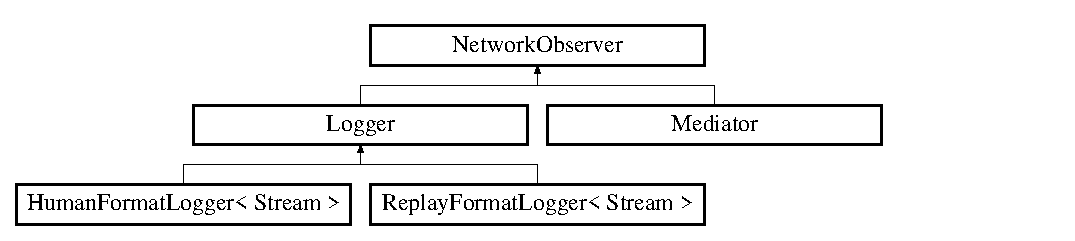
\includegraphics[height=2.786070cm]{classNetworkObserver}
\end{center}
\end{figure}
\subsection*{Public Member Functions}
\begin{DoxyCompactItemize}
\item 
\hypertarget{classNetworkObserver_a9eee41ce2b4dcc3ed580513dca0321b1}{
virtual void {\bfseries update} (NetworkUpdateContext context, const void $\ast$data)=0}
\label{classNetworkObserver_a9eee41ce2b4dcc3ed580513dca0321b1}

\end{DoxyCompactItemize}


The documentation for this class was generated from the following files:\begin{DoxyCompactItemize}
\item 
/home/kevin/workspace/HugMe/HugMe v0.9.1/Network/NetworkObserver.h\item 
/home/kevin/workspace/HugMe/HugMe v0.9.1/Network/NetworkObserver.cpp\end{DoxyCompactItemize}

\hypertarget{classNetworkReplayer}{
\section{NetworkReplayer Class Reference}
\label{classNetworkReplayer}\index{NetworkReplayer@{NetworkReplayer}}
}
Inheritance diagram for NetworkReplayer:\begin{figure}[H]
\begin{center}
\leavevmode
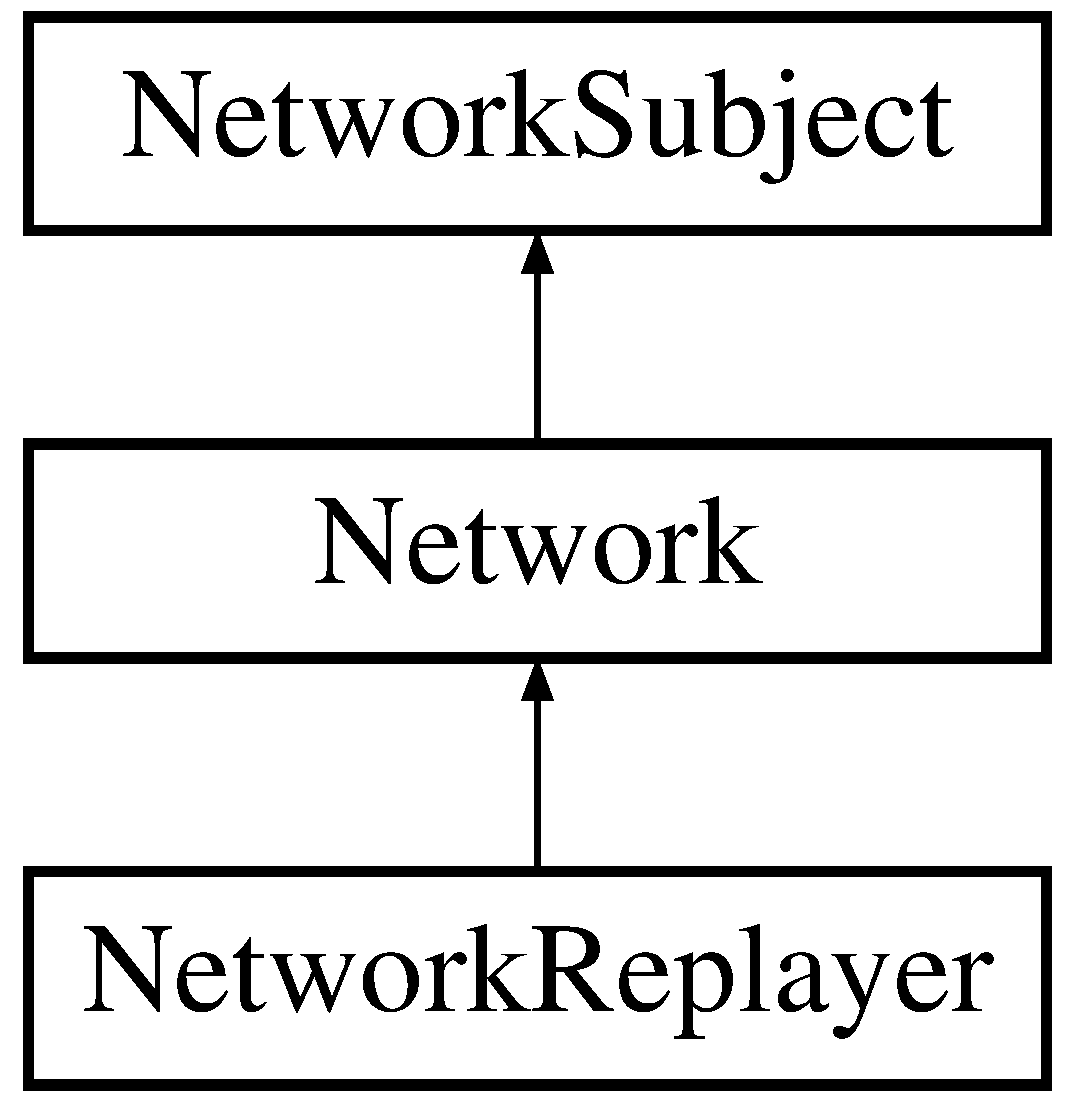
\includegraphics[height=3.000000cm]{classNetworkReplayer}
\end{center}
\end{figure}
\subsection*{Public Member Functions}
\begin{DoxyCompactItemize}
\item 
\hypertarget{classNetworkReplayer_ad91a8bed9fc2c9e69163c5290a823fee}{
{\bfseries NetworkReplayer} (boost::shared\_\-ptr$<$ std::ifstream $>$ file, boost::shared\_\-ptr$<$ boost::archive::text\_\-iarchive $>$ archive)}
\label{classNetworkReplayer_ad91a8bed9fc2c9e69163c5290a823fee}

\item 
\hypertarget{classNetworkReplayer_ab4162db2236a7b337bcef679682f8609}{
void {\bfseries replay} (LogEvent\_\-t logEvent)}
\label{classNetworkReplayer_ab4162db2236a7b337bcef679682f8609}

\item 
virtual rc\_\-network \hyperlink{classNetworkReplayer_a54f644fe92941370481c45989bad6615}{listen} (const std::string \&userName)
\begin{DoxyCompactList}\small\item\em Start listening for connections. \item\end{DoxyCompactList}\item 
virtual rc\_\-network \hyperlink{classNetworkReplayer_a6d4deeeede0cd5c07b44489a33c113f5}{connect} (const std::string \&ipAddress, const std::string \&userName)
\begin{DoxyCompactList}\small\item\em Attempt to connect to a peer. \item\end{DoxyCompactList}\item 
virtual rc\_\-network \hyperlink{classNetworkReplayer_a3aab774a33a87446aa874871fea54655}{disconnect} ()
\begin{DoxyCompactList}\small\item\em Disconnect from a peer. \item\end{DoxyCompactList}\item 
virtual rc\_\-network \hyperlink{classNetworkReplayer_aa9f70d4eee3d630c36c2bbc71bb7e195}{sendStartGame} ()
\begin{DoxyCompactList}\small\item\em Send a start game message to the peer. \item\end{DoxyCompactList}\item 
virtual rc\_\-network \hyperlink{classNetworkReplayer_aa54ba87a728ebdb0f23a82e409094468}{sendPauseGame} ()
\begin{DoxyCompactList}\small\item\em Send a pause game message to the peer. \item\end{DoxyCompactList}\item 
virtual rc\_\-network \hyperlink{classNetworkReplayer_a33c840b356485101092fe220d4aa73fb}{sendEndGame} ()
\begin{DoxyCompactList}\small\item\em Send an end game message to the peer. \item\end{DoxyCompactList}\item 
virtual rc\_\-network \hyperlink{classNetworkReplayer_a49bb75f65853c34c0bdafa6aba066056}{sendUserName} (const std::string \&userName)
\begin{DoxyCompactList}\small\item\em Send our username to the peer. \item\end{DoxyCompactList}\item 
virtual rc\_\-network \hyperlink{classNetworkReplayer_a689bc26f935bb0d7f72d3f69cea6e98c}{sendChatMessage} (const std::string \&message)
\begin{DoxyCompactList}\small\item\em Send a chat message to the peer. \item\end{DoxyCompactList}\item 
virtual rc\_\-network \hyperlink{classNetworkReplayer_ab7f69701316a3387da91d2146ea97b5e}{sendVideoData} (const \hyperlink{structVideoData}{VideoData} \&video)
\begin{DoxyCompactList}\small\item\em Send video data to the peer. \item\end{DoxyCompactList}\item 
virtual rc\_\-network \hyperlink{classNetworkReplayer_a7c9a5203b80840fee0157d506ff14f61}{sendPlayerPosition} (const cVector3d \&position)
\begin{DoxyCompactList}\small\item\em Send the players position to the peer. \item\end{DoxyCompactList}\item 
virtual rc\_\-network \hyperlink{classNetworkReplayer_ad8ad840c17aa86b890857ef714eb019a}{sendSlingshotPosition} (const cVector3d \&position)
\begin{DoxyCompactList}\small\item\em Send the slingshot position to the peer. \item\end{DoxyCompactList}\item 
virtual rc\_\-network \hyperlink{classNetworkReplayer_a7ebdbb74bb8e3b1fdc877d3c8157d342}{sendProjectile} (const \hyperlink{classProjectile}{Projectile} \&projectile)
\begin{DoxyCompactList}\small\item\em Send a projectile to the peer. \item\end{DoxyCompactList}\item 
virtual rc\_\-network \hyperlink{classNetworkReplayer_a98342ea3e802e9108b6d3329d977eade}{sendSlingshotPullback} ()
\begin{DoxyCompactList}\small\item\em Send a slingshot pullback event to the peer. \item\end{DoxyCompactList}\item 
\hypertarget{classNetworkReplayer_a8bc7c3c55dd7f7227d63335206a905a0}{
virtual rc\_\-network {\bfseries sendSlingshotRelease} ()}
\label{classNetworkReplayer_a8bc7c3c55dd7f7227d63335206a905a0}

\item 
virtual bool \hyperlink{classNetworkReplayer_a3656c06c32e76a30ac48055a0695d99a}{isConnected} () const 
\begin{DoxyCompactList}\small\item\em Determines if we are connected to a peer. \item\end{DoxyCompactList}\item 
virtual bool \hyperlink{classNetworkReplayer_a869c34b845f18eb262ead68542662aa4}{isListening} () const 
\begin{DoxyCompactList}\small\item\em Determines if we are listening for connections. \item\end{DoxyCompactList}\end{DoxyCompactItemize}


\subsection{Member Function Documentation}
\hypertarget{classNetworkReplayer_a6d4deeeede0cd5c07b44489a33c113f5}{
\index{NetworkReplayer@{NetworkReplayer}!connect@{connect}}
\index{connect@{connect}!NetworkReplayer@{NetworkReplayer}}
\subsubsection[{connect}]{\setlength{\rightskip}{0pt plus 5cm}rc\_\-network NetworkReplayer::connect (
\begin{DoxyParamCaption}
\item[{const std::string \&}]{ ipAddress, }
\item[{const std::string \&}]{ userName}
\end{DoxyParamCaption}
)\hspace{0.3cm}{\ttfamily  \mbox{[}virtual\mbox{]}}}}
\label{classNetworkReplayer_a6d4deeeede0cd5c07b44489a33c113f5}


Attempt to connect to a peer. 


\begin{DoxyParams}{Parameters}
\item[{\em ipAddress}]The ip address that we will connect to \item[{\em userName}]The username that will be used to establish the connection \end{DoxyParams}
\begin{DoxyReturn}{Returns}
The error code, SUCCESS if we are now connected to the peer 
\end{DoxyReturn}


Implements \hyperlink{classNetwork_a105f5e229e0ac9ff2b718dd34112c292}{Network}.

\hypertarget{classNetworkReplayer_a3aab774a33a87446aa874871fea54655}{
\index{NetworkReplayer@{NetworkReplayer}!disconnect@{disconnect}}
\index{disconnect@{disconnect}!NetworkReplayer@{NetworkReplayer}}
\subsubsection[{disconnect}]{\setlength{\rightskip}{0pt plus 5cm}rc\_\-network NetworkReplayer::disconnect (
\begin{DoxyParamCaption}
{}
\end{DoxyParamCaption}
)\hspace{0.3cm}{\ttfamily  \mbox{[}virtual\mbox{]}}}}
\label{classNetworkReplayer_a3aab774a33a87446aa874871fea54655}


Disconnect from a peer. 

\begin{DoxyReturn}{Returns}
The error code, SUCCESS if we successfully disconnected 
\end{DoxyReturn}


Implements \hyperlink{classNetwork_a1b0e29fc9936615e76c1db95caba0a9e}{Network}.

\hypertarget{classNetworkReplayer_a3656c06c32e76a30ac48055a0695d99a}{
\index{NetworkReplayer@{NetworkReplayer}!isConnected@{isConnected}}
\index{isConnected@{isConnected}!NetworkReplayer@{NetworkReplayer}}
\subsubsection[{isConnected}]{\setlength{\rightskip}{0pt plus 5cm}bool NetworkReplayer::isConnected (
\begin{DoxyParamCaption}
{}
\end{DoxyParamCaption}
) const\hspace{0.3cm}{\ttfamily  \mbox{[}virtual\mbox{]}}}}
\label{classNetworkReplayer_a3656c06c32e76a30ac48055a0695d99a}


Determines if we are connected to a peer. 

\begin{DoxyReturn}{Returns}
true if we are connected to a peer 
\end{DoxyReturn}


Implements \hyperlink{classNetwork_ab84ebbf03390c5ee99a27e2b340e3518}{Network}.

\hypertarget{classNetworkReplayer_a869c34b845f18eb262ead68542662aa4}{
\index{NetworkReplayer@{NetworkReplayer}!isListening@{isListening}}
\index{isListening@{isListening}!NetworkReplayer@{NetworkReplayer}}
\subsubsection[{isListening}]{\setlength{\rightskip}{0pt plus 5cm}bool NetworkReplayer::isListening (
\begin{DoxyParamCaption}
{}
\end{DoxyParamCaption}
) const\hspace{0.3cm}{\ttfamily  \mbox{[}virtual\mbox{]}}}}
\label{classNetworkReplayer_a869c34b845f18eb262ead68542662aa4}


Determines if we are listening for connections. 

\begin{DoxyReturn}{Returns}
true if we are listening for connections 
\end{DoxyReturn}


Implements \hyperlink{classNetwork_a1e8342d061f8e1b28d50d966e946650b}{Network}.

\hypertarget{classNetworkReplayer_a54f644fe92941370481c45989bad6615}{
\index{NetworkReplayer@{NetworkReplayer}!listen@{listen}}
\index{listen@{listen}!NetworkReplayer@{NetworkReplayer}}
\subsubsection[{listen}]{\setlength{\rightskip}{0pt plus 5cm}rc\_\-network NetworkReplayer::listen (
\begin{DoxyParamCaption}
\item[{const std::string \&}]{ userName}
\end{DoxyParamCaption}
)\hspace{0.3cm}{\ttfamily  \mbox{[}virtual\mbox{]}}}}
\label{classNetworkReplayer_a54f644fe92941370481c45989bad6615}


Start listening for connections. 


\begin{DoxyParams}{Parameters}
\item[{\em userName}]The username used to establish the connection \end{DoxyParams}
\begin{DoxyReturn}{Returns}
The error code, SUCCESS if listening was successful 
\end{DoxyReturn}


Implements \hyperlink{classNetwork_afb5306e2b769c01780aaa44d2c14306d}{Network}.

\hypertarget{classNetworkReplayer_a689bc26f935bb0d7f72d3f69cea6e98c}{
\index{NetworkReplayer@{NetworkReplayer}!sendChatMessage@{sendChatMessage}}
\index{sendChatMessage@{sendChatMessage}!NetworkReplayer@{NetworkReplayer}}
\subsubsection[{sendChatMessage}]{\setlength{\rightskip}{0pt plus 5cm}rc\_\-network NetworkReplayer::sendChatMessage (
\begin{DoxyParamCaption}
\item[{const std::string \&}]{ message}
\end{DoxyParamCaption}
)\hspace{0.3cm}{\ttfamily  \mbox{[}virtual\mbox{]}}}}
\label{classNetworkReplayer_a689bc26f935bb0d7f72d3f69cea6e98c}


Send a chat message to the peer. 


\begin{DoxyParams}{Parameters}
\item[{\em message}]The chat message that will be sent to the peer. \end{DoxyParams}
\begin{DoxyReturn}{Returns}
The error code, SUCCESS if the message was sent and received 
\end{DoxyReturn}


Implements \hyperlink{classNetwork_aa5e1e44e3cb4862b2c343999c89ce3b5}{Network}.

\hypertarget{classNetworkReplayer_a33c840b356485101092fe220d4aa73fb}{
\index{NetworkReplayer@{NetworkReplayer}!sendEndGame@{sendEndGame}}
\index{sendEndGame@{sendEndGame}!NetworkReplayer@{NetworkReplayer}}
\subsubsection[{sendEndGame}]{\setlength{\rightskip}{0pt plus 5cm}rc\_\-network NetworkReplayer::sendEndGame (
\begin{DoxyParamCaption}
{}
\end{DoxyParamCaption}
)\hspace{0.3cm}{\ttfamily  \mbox{[}virtual\mbox{]}}}}
\label{classNetworkReplayer_a33c840b356485101092fe220d4aa73fb}


Send an end game message to the peer. 

\begin{DoxyReturn}{Returns}
The error code, SUCCESS if the message was sent and received 
\end{DoxyReturn}


Implements \hyperlink{classNetwork_ae3f72f3003309c6d38105f504db8ce05}{Network}.

\hypertarget{classNetworkReplayer_aa54ba87a728ebdb0f23a82e409094468}{
\index{NetworkReplayer@{NetworkReplayer}!sendPauseGame@{sendPauseGame}}
\index{sendPauseGame@{sendPauseGame}!NetworkReplayer@{NetworkReplayer}}
\subsubsection[{sendPauseGame}]{\setlength{\rightskip}{0pt plus 5cm}rc\_\-network NetworkReplayer::sendPauseGame (
\begin{DoxyParamCaption}
{}
\end{DoxyParamCaption}
)\hspace{0.3cm}{\ttfamily  \mbox{[}virtual\mbox{]}}}}
\label{classNetworkReplayer_aa54ba87a728ebdb0f23a82e409094468}


Send a pause game message to the peer. 

\begin{DoxyReturn}{Returns}
The error code, SUCCESS if the message was sent and received 
\end{DoxyReturn}


Implements \hyperlink{classNetwork_ac60291a8d99468ebc38d085fc0455df0}{Network}.

\hypertarget{classNetworkReplayer_a7c9a5203b80840fee0157d506ff14f61}{
\index{NetworkReplayer@{NetworkReplayer}!sendPlayerPosition@{sendPlayerPosition}}
\index{sendPlayerPosition@{sendPlayerPosition}!NetworkReplayer@{NetworkReplayer}}
\subsubsection[{sendPlayerPosition}]{\setlength{\rightskip}{0pt plus 5cm}rc\_\-network NetworkReplayer::sendPlayerPosition (
\begin{DoxyParamCaption}
\item[{const cVector3d \&}]{ position}
\end{DoxyParamCaption}
)\hspace{0.3cm}{\ttfamily  \mbox{[}virtual\mbox{]}}}}
\label{classNetworkReplayer_a7c9a5203b80840fee0157d506ff14f61}


Send the players position to the peer. 


\begin{DoxyParams}{Parameters}
\item[{\em position}]Our player position that will be sent to the peer. \end{DoxyParams}
\begin{DoxyReturn}{Returns}
The error code, SUCCESS if the message was sent and received 
\end{DoxyReturn}


Implements \hyperlink{classNetwork_a9a2eb94c34d8d93f7490184cd2526e62}{Network}.

\hypertarget{classNetworkReplayer_a7ebdbb74bb8e3b1fdc877d3c8157d342}{
\index{NetworkReplayer@{NetworkReplayer}!sendProjectile@{sendProjectile}}
\index{sendProjectile@{sendProjectile}!NetworkReplayer@{NetworkReplayer}}
\subsubsection[{sendProjectile}]{\setlength{\rightskip}{0pt plus 5cm}rc\_\-network NetworkReplayer::sendProjectile (
\begin{DoxyParamCaption}
\item[{const {\bf Projectile} \&}]{ projectile}
\end{DoxyParamCaption}
)\hspace{0.3cm}{\ttfamily  \mbox{[}virtual\mbox{]}}}}
\label{classNetworkReplayer_a7ebdbb74bb8e3b1fdc877d3c8157d342}


Send a projectile to the peer. 


\begin{DoxyParams}{Parameters}
\item[{\em projectile}]The projectile that will be sent to the peer. \end{DoxyParams}
\begin{DoxyReturn}{Returns}
The error code, SUCCESS if the message was sent and received 
\end{DoxyReturn}


Implements \hyperlink{classNetwork_a477324500341f146fc7fc7411290a424}{Network}.

\hypertarget{classNetworkReplayer_ad8ad840c17aa86b890857ef714eb019a}{
\index{NetworkReplayer@{NetworkReplayer}!sendSlingshotPosition@{sendSlingshotPosition}}
\index{sendSlingshotPosition@{sendSlingshotPosition}!NetworkReplayer@{NetworkReplayer}}
\subsubsection[{sendSlingshotPosition}]{\setlength{\rightskip}{0pt plus 5cm}rc\_\-network NetworkReplayer::sendSlingshotPosition (
\begin{DoxyParamCaption}
\item[{const cVector3d \&}]{ position}
\end{DoxyParamCaption}
)\hspace{0.3cm}{\ttfamily  \mbox{[}virtual\mbox{]}}}}
\label{classNetworkReplayer_ad8ad840c17aa86b890857ef714eb019a}


Send the slingshot position to the peer. 


\begin{DoxyParams}{Parameters}
\item[{\em position}]Our slingshot position that will be sent to the peer. \end{DoxyParams}
\begin{DoxyReturn}{Returns}
The error code, SUCCESS if the message was sent and received 
\end{DoxyReturn}


Implements \hyperlink{classNetwork_aa105332ed8a1325a89f1f3e0a9d27521}{Network}.

\hypertarget{classNetworkReplayer_a98342ea3e802e9108b6d3329d977eade}{
\index{NetworkReplayer@{NetworkReplayer}!sendSlingshotPullback@{sendSlingshotPullback}}
\index{sendSlingshotPullback@{sendSlingshotPullback}!NetworkReplayer@{NetworkReplayer}}
\subsubsection[{sendSlingshotPullback}]{\setlength{\rightskip}{0pt plus 5cm}rc\_\-network NetworkReplayer::sendSlingshotPullback (
\begin{DoxyParamCaption}
{}
\end{DoxyParamCaption}
)\hspace{0.3cm}{\ttfamily  \mbox{[}virtual\mbox{]}}}}
\label{classNetworkReplayer_a98342ea3e802e9108b6d3329d977eade}


Send a slingshot pullback event to the peer. 

This lets the peer know that we have started to pull back our slingshot. \begin{DoxyReturn}{Returns}
The error code, SUCCESS if the message was sent and received 
\end{DoxyReturn}


Implements \hyperlink{classNetwork_ad4fd766e5bae5a3f002a26218b60b426}{Network}.

\hypertarget{classNetworkReplayer_aa9f70d4eee3d630c36c2bbc71bb7e195}{
\index{NetworkReplayer@{NetworkReplayer}!sendStartGame@{sendStartGame}}
\index{sendStartGame@{sendStartGame}!NetworkReplayer@{NetworkReplayer}}
\subsubsection[{sendStartGame}]{\setlength{\rightskip}{0pt plus 5cm}rc\_\-network NetworkReplayer::sendStartGame (
\begin{DoxyParamCaption}
{}
\end{DoxyParamCaption}
)\hspace{0.3cm}{\ttfamily  \mbox{[}virtual\mbox{]}}}}
\label{classNetworkReplayer_aa9f70d4eee3d630c36c2bbc71bb7e195}


Send a start game message to the peer. 

\begin{DoxyReturn}{Returns}
The error code, SUCCESS if the message was sent and received 
\end{DoxyReturn}


Implements \hyperlink{classNetwork_a3f6b451fd546f2e44eb2c14661bc1ad3}{Network}.

\hypertarget{classNetworkReplayer_a49bb75f65853c34c0bdafa6aba066056}{
\index{NetworkReplayer@{NetworkReplayer}!sendUserName@{sendUserName}}
\index{sendUserName@{sendUserName}!NetworkReplayer@{NetworkReplayer}}
\subsubsection[{sendUserName}]{\setlength{\rightskip}{0pt plus 5cm}rc\_\-network NetworkReplayer::sendUserName (
\begin{DoxyParamCaption}
\item[{const std::string \&}]{ userName}
\end{DoxyParamCaption}
)\hspace{0.3cm}{\ttfamily  \mbox{[}virtual\mbox{]}}}}
\label{classNetworkReplayer_a49bb75f65853c34c0bdafa6aba066056}


Send our username to the peer. 

The user name is sent when the connection is established so this should only be used if a user changes there username 
\begin{DoxyParams}{Parameters}
\item[{\em userName}]Our new username that will be sent to the peer \end{DoxyParams}
\begin{DoxyReturn}{Returns}
The error code, SUCCESS if the message was sent and received 
\end{DoxyReturn}


Implements \hyperlink{classNetwork_a741e75b2e9adfc188c53e150b4dd4610}{Network}.

\hypertarget{classNetworkReplayer_ab7f69701316a3387da91d2146ea97b5e}{
\index{NetworkReplayer@{NetworkReplayer}!sendVideoData@{sendVideoData}}
\index{sendVideoData@{sendVideoData}!NetworkReplayer@{NetworkReplayer}}
\subsubsection[{sendVideoData}]{\setlength{\rightskip}{0pt plus 5cm}rc\_\-network NetworkReplayer::sendVideoData (
\begin{DoxyParamCaption}
\item[{const {\bf VideoData} \&}]{ video}
\end{DoxyParamCaption}
)\hspace{0.3cm}{\ttfamily  \mbox{[}virtual\mbox{]}}}}
\label{classNetworkReplayer_ab7f69701316a3387da91d2146ea97b5e}


Send video data to the peer. 


\begin{DoxyParams}{Parameters}
\item[{\em video}]The video data that will be sent to the peer. \end{DoxyParams}
\begin{DoxyReturn}{Returns}
The error code, SUCCESS if the message was sent and received 
\end{DoxyReturn}


Implements \hyperlink{classNetwork_a189df8819d21d4f1a277ca753453045b}{Network}.



The documentation for this class was generated from the following files:\begin{DoxyCompactItemize}
\item 
/home/kevin/workspace/HugMe/HugMe v0.9.1/Replay/NetworkReplayer.h\item 
/home/kevin/workspace/HugMe/HugMe v0.9.1/Replay/NetworkReplayer.cpp\end{DoxyCompactItemize}

\hypertarget{classNetworkSocket}{
\section{NetworkSocket Class Reference}
\label{classNetworkSocket}\index{NetworkSocket@{NetworkSocket}}
}
\subsection*{Public Member Functions}
\begin{DoxyCompactItemize}
\item 
\hypertarget{classNetworkSocket_acdeaa6046b82c34b052231e83ed52632}{
{\bfseries NetworkSocket} (\hyperlink{classWinsockNetwork}{WinsockNetwork} $\ast$network)}
\label{classNetworkSocket_acdeaa6046b82c34b052231e83ed52632}

\item 
\hypertarget{classNetworkSocket_a9ac28b209fad28645fd7d92d23c98c75}{
virtual SOCKET {\bfseries Detach} ()}
\label{classNetworkSocket_a9ac28b209fad28645fd7d92d23c98c75}

\item 
\hypertarget{classNetworkSocket_a1a7420b1acbee18bd95d530e6c4867e7}{
virtual bool {\bfseries isServer} () const }
\label{classNetworkSocket_a1a7420b1acbee18bd95d530e6c4867e7}

\item 
\hypertarget{classNetworkSocket_a2f5d8b1ef1b262fd6106b59344e4af3d}{
virtual void {\bfseries OnAccept} (int nErrorCode)}
\label{classNetworkSocket_a2f5d8b1ef1b262fd6106b59344e4af3d}

\end{DoxyCompactItemize}


The documentation for this class was generated from the following files:\begin{DoxyCompactItemize}
\item 
/home/kevin/workspace/HugMe/HugMe v0.9.1/Network/NetworkSocket.h\item 
/home/kevin/workspace/HugMe/HugMe v0.9.1/Network/NetworkSocket.cpp\end{DoxyCompactItemize}

\hypertarget{classNetworkSubject}{
\section{NetworkSubject Class Reference}
\label{classNetworkSubject}\index{NetworkSubject@{NetworkSubject}}
}
Inheritance diagram for NetworkSubject:\begin{figure}[H]
\begin{center}
\leavevmode
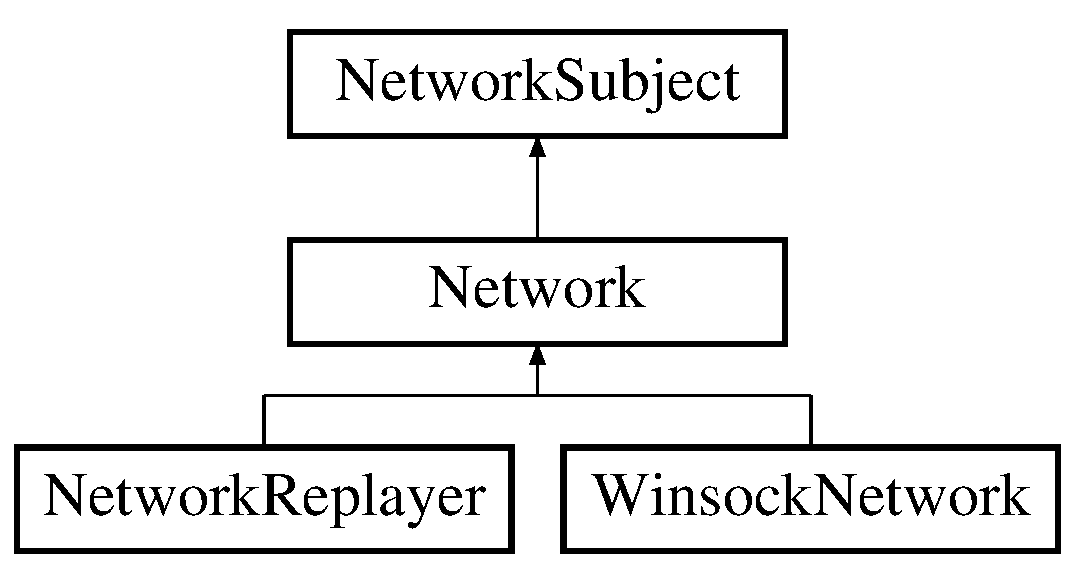
\includegraphics[height=3.000000cm]{classNetworkSubject}
\end{center}
\end{figure}
\subsection*{Public Member Functions}
\begin{DoxyCompactItemize}
\item 
\hypertarget{classNetworkSubject_a7dad1909bc12d5bba33ac9b935f39465}{
void {\bfseries attach} (\hyperlink{classNetworkObserver}{NetworkObserver} $\ast$observer)}
\label{classNetworkSubject_a7dad1909bc12d5bba33ac9b935f39465}

\item 
\hypertarget{classNetworkSubject_a9c2121db78ea8b1d1d3e3ab5e709a081}{
void {\bfseries detach} (\hyperlink{classNetworkObserver}{NetworkObserver} $\ast$observer)}
\label{classNetworkSubject_a9c2121db78ea8b1d1d3e3ab5e709a081}

\item 
\hypertarget{classNetworkSubject_abcf72266c492400152874107c6f2cc25}{
void {\bfseries notify} (NetworkUpdateContext context, const void $\ast$data=NULL)}
\label{classNetworkSubject_abcf72266c492400152874107c6f2cc25}

\end{DoxyCompactItemize}


The documentation for this class was generated from the following files:\begin{DoxyCompactItemize}
\item 
/home/kevin/workspace/HugMe/HugMe v0.9.1/Network/NetworkSubject.h\item 
/home/kevin/workspace/HugMe/HugMe v0.9.1/Network/NetworkSubject.cpp\end{DoxyCompactItemize}

\hypertarget{classNovintFalcon}{
\section{NovintFalcon Class Reference}
\label{classNovintFalcon}\index{NovintFalcon@{NovintFalcon}}
}


The novint falcon.  




{\ttfamily \#include $<$NovintFalcon.h$>$}

Inheritance diagram for NovintFalcon:\begin{figure}[H]
\begin{center}
\leavevmode
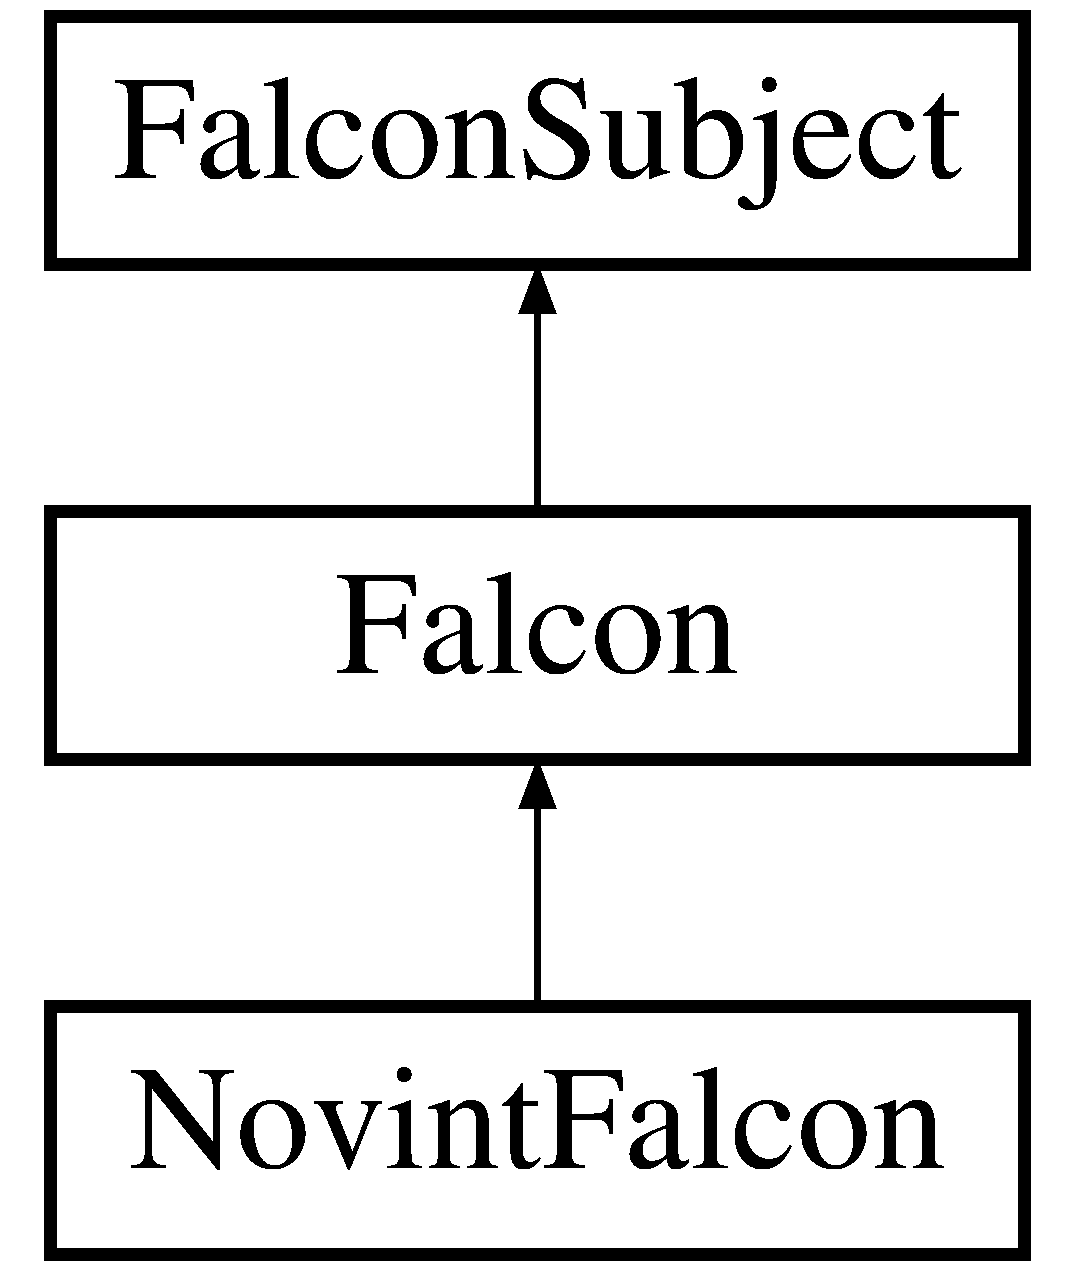
\includegraphics[height=3.000000cm]{classNovintFalcon}
\end{center}
\end{figure}
\subsection*{Public Member Functions}
\begin{DoxyCompactItemize}
\item 
\hyperlink{classNovintFalcon_ac36e7148131ecbdfff97289f2c9e3b9c}{NovintFalcon} ()
\begin{DoxyCompactList}\small\item\em Constructor. \item\end{DoxyCompactList}\item 
\hypertarget{classNovintFalcon_afb0ece97317db2eb6da852e219cc85eb}{
virtual \hyperlink{classNovintFalcon_afb0ece97317db2eb6da852e219cc85eb}{$\sim$NovintFalcon} ()}
\label{classNovintFalcon_afb0ece97317db2eb6da852e219cc85eb}

\begin{DoxyCompactList}\small\item\em Destructor. \item\end{DoxyCompactList}\item 
\hypertarget{classNovintFalcon_a3e82b6e9d7c393684b809971208922bf}{
virtual void \hyperlink{classNovintFalcon_a3e82b6e9d7c393684b809971208922bf}{startPolling} ()}
\label{classNovintFalcon_a3e82b6e9d7c393684b809971208922bf}

\begin{DoxyCompactList}\small\item\em Start polling the falcon for information. \item\end{DoxyCompactList}\item 
\hypertarget{classNovintFalcon_a3bc94cd6f05df1d327f79fb87001039d}{
virtual void \hyperlink{classNovintFalcon_a3bc94cd6f05df1d327f79fb87001039d}{stopPolling} ()}
\label{classNovintFalcon_a3bc94cd6f05df1d327f79fb87001039d}

\begin{DoxyCompactList}\small\item\em Stop polling the falcon for information. \item\end{DoxyCompactList}\item 
virtual cCollisionAABBBox \hyperlink{classNovintFalcon_a8226c5b4a2cb0d2e88b6a41e2c7c3af9}{boundingBox} () const 
\begin{DoxyCompactList}\small\item\em Returns the box to which the slingshot is bound. \item\end{DoxyCompactList}\end{DoxyCompactItemize}


\subsection{Detailed Description}
The novint falcon. This class controls the slingshot via a novint falcon. 

\subsection{Constructor \& Destructor Documentation}
\hypertarget{classNovintFalcon_ac36e7148131ecbdfff97289f2c9e3b9c}{
\index{NovintFalcon@{NovintFalcon}!NovintFalcon@{NovintFalcon}}
\index{NovintFalcon@{NovintFalcon}!NovintFalcon@{NovintFalcon}}
\subsubsection[{NovintFalcon}]{\setlength{\rightskip}{0pt plus 5cm}NovintFalcon::NovintFalcon (
\begin{DoxyParamCaption}
{}
\end{DoxyParamCaption}
)}}
\label{classNovintFalcon_ac36e7148131ecbdfff97289f2c9e3b9c}


Constructor. 



Local slingshot bounding box



\subsection{Member Function Documentation}
\hypertarget{classNovintFalcon_a8226c5b4a2cb0d2e88b6a41e2c7c3af9}{
\index{NovintFalcon@{NovintFalcon}!boundingBox@{boundingBox}}
\index{boundingBox@{boundingBox}!NovintFalcon@{NovintFalcon}}
\subsubsection[{boundingBox}]{\setlength{\rightskip}{0pt plus 5cm}cCollisionAABBBox NovintFalcon::boundingBox (
\begin{DoxyParamCaption}
{}
\end{DoxyParamCaption}
) const\hspace{0.3cm}{\ttfamily  \mbox{[}virtual\mbox{]}}}}
\label{classNovintFalcon_a8226c5b4a2cb0d2e88b6a41e2c7c3af9}


Returns the box to which the slingshot is bound. 

\begin{DoxyReturn}{Returns}
the box to which the slingshot is bound 
\end{DoxyReturn}


Implements \hyperlink{classFalcon_a8113221c67437ed4f726af6d68c0e66e}{Falcon}.



The documentation for this class was generated from the following files:\begin{DoxyCompactItemize}
\item 
/home/kevin/workspace/HugMe/HugMe v0.9.1/Falcon/NovintFalcon.h\item 
/home/kevin/workspace/HugMe/HugMe v0.9.1/Falcon/NovintFalcon.cpp\end{DoxyCompactItemize}

\hypertarget{classOfficeSlingshot3D}{
\section{OfficeSlingshot3D Class Reference}
\label{classOfficeSlingshot3D}\index{OfficeSlingshot3D@{OfficeSlingshot3D}}
}
\subsection*{Public Member Functions}
\begin{DoxyCompactItemize}
\item 
\hypertarget{classOfficeSlingshot3D_a3695f1459a3979777d0f06fdcbdde7a1}{
{\bfseries OfficeSlingshot3D} (boost::shared\_\-ptr$<$ \hyperlink{classGame}{Game} $>$ game, boost::shared\_\-ptr$<$ \hyperlink{classLogger}{Logger} $>$ logger, boost::shared\_\-ptr$<$ \hyperlink{classReplayer}{Replayer} $>$ replayer, CDialog $\ast$dialog)}
\label{classOfficeSlingshot3D_a3695f1459a3979777d0f06fdcbdde7a1}

\item 
\hypertarget{classOfficeSlingshot3D_a0f34ade76b08ebb126176bca57eaec66}{
void {\bfseries run} ()}
\label{classOfficeSlingshot3D_a0f34ade76b08ebb126176bca57eaec66}

\item 
\hypertarget{classOfficeSlingshot3D_a525fe6fecb5ec28394dfe906596a5421}{
void {\bfseries operator()} ()}
\label{classOfficeSlingshot3D_a525fe6fecb5ec28394dfe906596a5421}

\end{DoxyCompactItemize}


The documentation for this class was generated from the following files:\begin{DoxyCompactItemize}
\item 
/home/kevin/workspace/HugMe/HugMe v0.9.1/Main/OfficeSlingshot3D.h\item 
/home/kevin/workspace/HugMe/HugMe v0.9.1/Main/OfficeSlingshot3D.cpp\end{DoxyCompactItemize}

\hypertarget{classOfficeSlingshot3DFactory}{
\section{OfficeSlingshot3DFactory Class Reference}
\label{classOfficeSlingshot3DFactory}\index{OfficeSlingshot3DFactory@{OfficeSlingshot3DFactory}}
}
\subsection*{Static Public Member Functions}
\begin{DoxyCompactItemize}
\item 
\hypertarget{classOfficeSlingshot3DFactory_ae282fe62015e22275188d157d9fa5fcb}{
static boost::shared\_\-ptr$<$ \hyperlink{classOfficeSlingshot3D}{OfficeSlingshot3D} $>$ {\bfseries createFromConfigFile} (const std::string \&fileName)}
\label{classOfficeSlingshot3DFactory_ae282fe62015e22275188d157d9fa5fcb}

\end{DoxyCompactItemize}


The documentation for this class was generated from the following files:\begin{DoxyCompactItemize}
\item 
/home/kevin/workspace/HugMe/HugMe v0.9.1/Main/OfficeSlingshot3DFactory.h\item 
/home/kevin/workspace/HugMe/HugMe v0.9.1/Main/OfficeSlingshot3DFactory.cpp\end{DoxyCompactItemize}

\hypertarget{classPacket}{
\section{Packet$<$ PacketType $>$ Class Template Reference}
\label{classPacket}\index{Packet@{Packet}}
}
\subsection*{Public Member Functions}
\begin{DoxyCompactItemize}
\item 
\hypertarget{classPacket_ad1c9f433dbc7a5ba43bbdff826fb1dd7}{
PacketType {\bfseries getType} () const }
\label{classPacket_ad1c9f433dbc7a5ba43bbdff826fb1dd7}

\item 
\hypertarget{classPacket_af688d0ad264f65b12c9cdc999218a828}{
boost::shared\_\-ptr$<$ const std::vector$<$ char $>$ $>$ {\bfseries getHeader} () const }
\label{classPacket_af688d0ad264f65b12c9cdc999218a828}

\item 
\hypertarget{classPacket_a96a63681049b3d47e2f0252336c8e6ef}{
boost::shared\_\-ptr$<$ const std::vector$<$ char $>$ $>$ {\bfseries getData} () const }
\label{classPacket_a96a63681049b3d47e2f0252336c8e6ef}

\item 
\hypertarget{classPacket_ae2b47f4d54170c708dd50edf95e167b7}{
bool {\bfseries readPacket} (std::vector$<$ char $>$ \&input)}
\label{classPacket_ae2b47f4d54170c708dd50edf95e167b7}

\item 
\hypertarget{classPacket_a95ca1c18efc8202f7cd4c46ffb89a4a8}{
{\footnotesize template$<$typename T $>$ }\\void {\bfseries write} (PacketType type, const T \&t)}
\label{classPacket_a95ca1c18efc8202f7cd4c46ffb89a4a8}

\item 
\hypertarget{classPacket_a42af3a3916922f11ab4bcc4f88ed959b}{
void {\bfseries write} (PacketType type, const \hyperlink{structVideoData}{VideoData} \&video)}
\label{classPacket_a42af3a3916922f11ab4bcc4f88ed959b}

\item 
\hypertarget{classPacket_a28002ec8b26d8d6affcabdcab11ba0a0}{
void {\bfseries write} (PacketType type)}
\label{classPacket_a28002ec8b26d8d6affcabdcab11ba0a0}

\item 
\hypertarget{classPacket_a0f40b9784dca6e16c6a64ee2d882e670}{
{\footnotesize template$<$typename T $>$ }\\void {\bfseries read} (T \&t) const }
\label{classPacket_a0f40b9784dca6e16c6a64ee2d882e670}

\item 
\hypertarget{classPacket_ab6d8226bd69d08362da8402646c14045}{
void {\bfseries read} (\hyperlink{structVideoData}{VideoData} \&video) const }
\label{classPacket_ab6d8226bd69d08362da8402646c14045}

\item 
\hypertarget{classPacket_aeaa7b195cad3722b9f4e39093e8193e5}{
void {\bfseries clear} ()}
\label{classPacket_aeaa7b195cad3722b9f4e39093e8193e5}

\end{DoxyCompactItemize}
\subsubsection*{template$<$typename PacketType$>$ class Packet$<$ PacketType $>$}



The documentation for this class was generated from the following file:\begin{DoxyCompactItemize}
\item 
/home/kevin/workspace/HugMe/HugMe v0.9.1/Network/Packet.h\end{DoxyCompactItemize}

\hypertarget{structPacketHeader}{
\section{PacketHeader$<$ PacketType $>$ Struct Template Reference}
\label{structPacketHeader}\index{PacketHeader@{PacketHeader}}
}
\subsection*{Data Fields}
\begin{DoxyCompactItemize}
\item 
\hypertarget{structPacketHeader_aa9dea8d798186486a554a72e5cccf251}{
unsigned int {\bfseries size}}
\label{structPacketHeader_aa9dea8d798186486a554a72e5cccf251}

\item 
\hypertarget{structPacketHeader_a05d799894147a984d82cf048788df180}{
PacketType {\bfseries type}}
\label{structPacketHeader_a05d799894147a984d82cf048788df180}

\end{DoxyCompactItemize}
\subsubsection*{template$<$typename PacketType$>$ struct PacketHeader$<$ PacketType $>$}



The documentation for this struct was generated from the following file:\begin{DoxyCompactItemize}
\item 
/home/kevin/workspace/HugMe/HugMe v0.9.1/Network/Packet.h\end{DoxyCompactItemize}

\hypertarget{classPerspectiveMath}{
\section{PerspectiveMath Class Reference}
\label{classPerspectiveMath}\index{PerspectiveMath@{PerspectiveMath}}
}


Utility class that the mediator will use to adjust the players perspectives so that they match.  




{\ttfamily \#include $<$PerspectiveMath.h$>$}

\subsection*{Static Public Member Functions}
\begin{DoxyCompactItemize}
\item 
static void \hyperlink{classPerspectiveMath_a65c41921db4ee62a8f3a92fb887cc8ce}{invert2DCoordinate} (cVector3d \&vector)
\begin{DoxyCompactList}\small\item\em Invert the perspective on a coordinate in a 2D space. \item\end{DoxyCompactList}\item 
static void \hyperlink{classPerspectiveMath_a37100d823fa9ed299d9987fd38c9e1f5}{invert3DCoordinate} (cVector3d \&vector)
\begin{DoxyCompactList}\small\item\em Invert the perspective on a coordinate in a 3D space. \item\end{DoxyCompactList}\item 
static void \hyperlink{classPerspectiveMath_a13cbb76a51ce78db12d4013b96586bd1}{invert3DProjectile} (\hyperlink{classProjectile}{Projectile} \&projectile)
\begin{DoxyCompactList}\small\item\em Invert the perspective on a projectile traveling in a 3D space. \item\end{DoxyCompactList}\item 
\hypertarget{classPerspectiveMath_a3a535221683e28fc95c5edae6c15d360}{
static void {\bfseries convertOrientationXYZtoYZX} (cVector3d \&vector)}
\label{classPerspectiveMath_a3a535221683e28fc95c5edae6c15d360}

\item 
\hypertarget{classPerspectiveMath_aa8fa5bbda93edd97ee3f0c280914fa6b}{
static void {\bfseries convertBoxToBox} (cVector3d \&vector, const cCollisionAABBBox \&boxOrigin, const cCollisionAABBBox \&boxTarget)}
\label{classPerspectiveMath_aa8fa5bbda93edd97ee3f0c280914fa6b}

\end{DoxyCompactItemize}


\subsection{Detailed Description}
Utility class that the mediator will use to adjust the players perspectives so that they match. 

\subsection{Member Function Documentation}
\hypertarget{classPerspectiveMath_a65c41921db4ee62a8f3a92fb887cc8ce}{
\index{PerspectiveMath@{PerspectiveMath}!invert2DCoordinate@{invert2DCoordinate}}
\index{invert2DCoordinate@{invert2DCoordinate}!PerspectiveMath@{PerspectiveMath}}
\subsubsection[{invert2DCoordinate}]{\setlength{\rightskip}{0pt plus 5cm}void PerspectiveMath::invert2DCoordinate (
\begin{DoxyParamCaption}
\item[{cVector3d \&}]{ vector}
\end{DoxyParamCaption}
)\hspace{0.3cm}{\ttfamily  \mbox{[}static\mbox{]}}}}
\label{classPerspectiveMath_a65c41921db4ee62a8f3a92fb887cc8ce}


Invert the perspective on a coordinate in a 2D space. 


\begin{DoxyParams}{Parameters}
\item[{\em vector}]The coordinate to invert \end{DoxyParams}
\hypertarget{classPerspectiveMath_a37100d823fa9ed299d9987fd38c9e1f5}{
\index{PerspectiveMath@{PerspectiveMath}!invert3DCoordinate@{invert3DCoordinate}}
\index{invert3DCoordinate@{invert3DCoordinate}!PerspectiveMath@{PerspectiveMath}}
\subsubsection[{invert3DCoordinate}]{\setlength{\rightskip}{0pt plus 5cm}void PerspectiveMath::invert3DCoordinate (
\begin{DoxyParamCaption}
\item[{cVector3d \&}]{ vector}
\end{DoxyParamCaption}
)\hspace{0.3cm}{\ttfamily  \mbox{[}static\mbox{]}}}}
\label{classPerspectiveMath_a37100d823fa9ed299d9987fd38c9e1f5}


Invert the perspective on a coordinate in a 3D space. 


\begin{DoxyParams}{Parameters}
\item[{\em vector}]The coordinate to invert \end{DoxyParams}
\hypertarget{classPerspectiveMath_a13cbb76a51ce78db12d4013b96586bd1}{
\index{PerspectiveMath@{PerspectiveMath}!invert3DProjectile@{invert3DProjectile}}
\index{invert3DProjectile@{invert3DProjectile}!PerspectiveMath@{PerspectiveMath}}
\subsubsection[{invert3DProjectile}]{\setlength{\rightskip}{0pt plus 5cm}void PerspectiveMath::invert3DProjectile (
\begin{DoxyParamCaption}
\item[{{\bf Projectile} \&}]{ projectile}
\end{DoxyParamCaption}
)\hspace{0.3cm}{\ttfamily  \mbox{[}static\mbox{]}}}}
\label{classPerspectiveMath_a13cbb76a51ce78db12d4013b96586bd1}


Invert the perspective on a projectile traveling in a 3D space. 


\begin{DoxyParams}{Parameters}
\item[{\em projectile}]The projectile to invert \end{DoxyParams}


The documentation for this class was generated from the following files:\begin{DoxyCompactItemize}
\item 
/home/kevin/workspace/HugMe/HugMe v0.9.1/Mediator/PerspectiveMath.h\item 
/home/kevin/workspace/HugMe/HugMe v0.9.1/Mediator/PerspectiveMath.cpp\end{DoxyCompactItemize}

\hypertarget{classProjectile}{
\section{Projectile Class Reference}
\label{classProjectile}\index{Projectile@{Projectile}}
}
\subsection*{Public Member Functions}
\begin{DoxyCompactItemize}
\item 
\hypertarget{classProjectile_ae83eedae52dc89c07f13d9af3844c0de}{
{\bfseries Projectile} (cVector3d position, cVector3d speed)}
\label{classProjectile_ae83eedae52dc89c07f13d9af3844c0de}

\item 
\hypertarget{classProjectile_aa55d774bc476f9612a4cdf6bbe886458}{
cVector3d {\bfseries getPosition} () const }
\label{classProjectile_aa55d774bc476f9612a4cdf6bbe886458}

\item 
\hypertarget{classProjectile_ab296c86308ef3ee4d4fc62a3379ebf8b}{
void {\bfseries setPosition} (double x, double y, double z)}
\label{classProjectile_ab296c86308ef3ee4d4fc62a3379ebf8b}

\item 
\hypertarget{classProjectile_ab1ae409448bf2ef3bb96a639621fcb46}{
void {\bfseries setPosition} (const cVector3d \&v)}
\label{classProjectile_ab1ae409448bf2ef3bb96a639621fcb46}

\item 
\hypertarget{classProjectile_a2bb207bbf1c0244f0e896de5950ee6b1}{
cVector3d {\bfseries getSpeed} () const }
\label{classProjectile_a2bb207bbf1c0244f0e896de5950ee6b1}

\item 
\hypertarget{classProjectile_a290fb17761a6a523df80791413c1f7b5}{
void {\bfseries setSpeed} (double x, double y, double z)}
\label{classProjectile_a290fb17761a6a523df80791413c1f7b5}

\item 
\hypertarget{classProjectile_a0564d5a2db445e6abf2423f19624f4fb}{
void {\bfseries setSpeed} (const cVector3d \&v)}
\label{classProjectile_a0564d5a2db445e6abf2423f19624f4fb}

\end{DoxyCompactItemize}
\subsection*{Friends}
\begin{DoxyCompactItemize}
\item 
\hypertarget{classProjectile_ac98d07dd8f7b70e16ccb9a01abf56b9c}{
class {\bfseries boost::serialization::access}}
\label{classProjectile_ac98d07dd8f7b70e16ccb9a01abf56b9c}

\end{DoxyCompactItemize}


The documentation for this class was generated from the following files:\begin{DoxyCompactItemize}
\item 
/home/kevin/workspace/HugMe/HugMe v0.9.1/Common/Projectile.h\item 
/home/kevin/workspace/HugMe/HugMe v0.9.1/Common/Projectile.cpp\end{DoxyCompactItemize}

\hypertarget{classReplayer}{
\section{Replayer Class Reference}
\label{classReplayer}\index{Replayer@{Replayer}}
}
\subsection*{Public Member Functions}
\begin{DoxyCompactItemize}
\item 
\hypertarget{classReplayer_a233ae971345bbadd96ecb5d868800ed8}{
{\bfseries Replayer} (const std::string \&fileName, const \hyperlink{structUserPreferences}{UserPreferences} \&preferences)}
\label{classReplayer_a233ae971345bbadd96ecb5d868800ed8}

\item 
\hypertarget{classReplayer_aaeeb2f5ae160cf99f8e07401c906d07f}{
void {\bfseries startReplay} ()}
\label{classReplayer_aaeeb2f5ae160cf99f8e07401c906d07f}

\item 
\hypertarget{classReplayer_abf2424525cedca13f7321f59036a403c}{
void {\bfseries stopReplay} ()}
\label{classReplayer_abf2424525cedca13f7321f59036a403c}

\item 
\hypertarget{classReplayer_a6d15b7b0bc222b486ddf2b86cb12e1cb}{
boost::shared\_\-ptr$<$ \hyperlink{classNetworkReplayer}{NetworkReplayer} $>$ {\bfseries getNetworkReplayer} ()}
\label{classReplayer_a6d15b7b0bc222b486ddf2b86cb12e1cb}

\item 
\hypertarget{classReplayer_a272dafad83fa64f509fbe1db67ed0e0c}{
boost::shared\_\-ptr$<$ \hyperlink{classUserInterfaceReplayer}{UserInterfaceReplayer} $>$ {\bfseries getUserInterfaceReplayer} ()}
\label{classReplayer_a272dafad83fa64f509fbe1db67ed0e0c}

\item 
\hypertarget{classReplayer_a472e6ebecd1f0ea89d6bd19d1ab79102}{
boost::shared\_\-ptr$<$ \hyperlink{classFalconReplayer}{FalconReplayer} $>$ {\bfseries getFalconReplayer} ()}
\label{classReplayer_a472e6ebecd1f0ea89d6bd19d1ab79102}

\item 
\hypertarget{classReplayer_a56299bc514f243c88da07fe0260e5eab}{
boost::shared\_\-ptr$<$ \hyperlink{classZCameraReplayer}{ZCameraReplayer} $>$ {\bfseries getZCameraReplayer} ()}
\label{classReplayer_a56299bc514f243c88da07fe0260e5eab}

\end{DoxyCompactItemize}


The documentation for this class was generated from the following files:\begin{DoxyCompactItemize}
\item 
/home/kevin/workspace/HugMe/HugMe v0.9.1/Replay/Replayer.h\item 
/home/kevin/workspace/HugMe/HugMe v0.9.1/Replay/Replayer.cpp\end{DoxyCompactItemize}

\hypertarget{classReplayFormatEvent}{
\section{ReplayFormatEvent Class Reference}
\label{classReplayFormatEvent}\index{ReplayFormatEvent@{ReplayFormatEvent}}
}
\subsection*{Public Member Functions}
\begin{DoxyCompactItemize}
\item 
\hypertarget{classReplayFormatEvent_aefd3a06940ae986aa9c3c2b6886cf5c2}{
{\bfseries ReplayFormatEvent} (long time, LogEvent\_\-t logEvent)}
\label{classReplayFormatEvent_aefd3a06940ae986aa9c3c2b6886cf5c2}

\end{DoxyCompactItemize}
\subsection*{Data Fields}
\begin{DoxyCompactItemize}
\item 
\hypertarget{classReplayFormatEvent_a8752c98de9f608ef9794efca7f08bdb9}{
long {\bfseries time}}
\label{classReplayFormatEvent_a8752c98de9f608ef9794efca7f08bdb9}

\item 
\hypertarget{classReplayFormatEvent_ad5f6fcaac9f58026e5a87a1320666236}{
LogEvent\_\-t {\bfseries logEvent}}
\label{classReplayFormatEvent_ad5f6fcaac9f58026e5a87a1320666236}

\end{DoxyCompactItemize}
\subsection*{Friends}
\begin{DoxyCompactItemize}
\item 
\hypertarget{classReplayFormatEvent_ac98d07dd8f7b70e16ccb9a01abf56b9c}{
class {\bfseries boost::serialization::access}}
\label{classReplayFormatEvent_ac98d07dd8f7b70e16ccb9a01abf56b9c}

\end{DoxyCompactItemize}


The documentation for this class was generated from the following files:\begin{DoxyCompactItemize}
\item 
/home/kevin/workspace/HugMe/HugMe v0.9.1/Logger/ReplayFormatEvent.h\item 
/home/kevin/workspace/HugMe/HugMe v0.9.1/Logger/ReplayFormatEvent.cpp\end{DoxyCompactItemize}

\hypertarget{classReplayFormatLogger}{
\section{ReplayFormatLogger$<$ Stream $>$ Class Template Reference}
\label{classReplayFormatLogger}\index{ReplayFormatLogger@{ReplayFormatLogger}}
}
Inheritance diagram for ReplayFormatLogger$<$ Stream $>$:\begin{figure}[H]
\begin{center}
\leavevmode
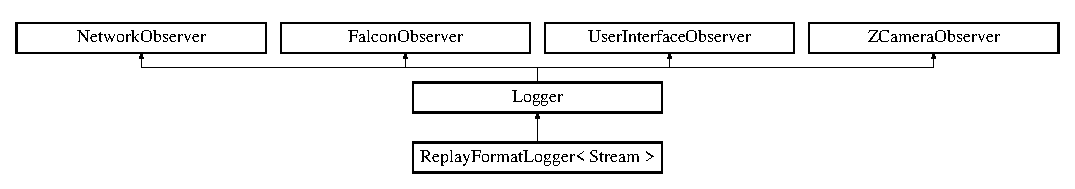
\includegraphics[height=2.089552cm]{classReplayFormatLogger}
\end{center}
\end{figure}
\subsection*{Public Member Functions}
\begin{DoxyCompactItemize}
\item 
\hypertarget{classReplayFormatLogger_a63a0043e0c400decedb7403780901159}{
{\footnotesize template$<$typename T1 $>$ }\\{\bfseries ReplayFormatLogger} (T1 param)}
\label{classReplayFormatLogger_a63a0043e0c400decedb7403780901159}

\item 
\hypertarget{classReplayFormatLogger_a2a048b2c87b25c64ed95fa9c6904ff61}{
{\footnotesize template$<$typename T1 , typename T2 $>$ }\\{\bfseries ReplayFormatLogger} (T1 param1, T2 param2)}
\label{classReplayFormatLogger_a2a048b2c87b25c64ed95fa9c6904ff61}

\item 
\hypertarget{classReplayFormatLogger_a767584e0a4ada86bf9012bd3279a77ac}{
{\footnotesize template$<$typename T1 , typename T2 , typename T3 $>$ }\\{\bfseries ReplayFormatLogger} (T1 param1, T2 param2, T3 param3)}
\label{classReplayFormatLogger_a767584e0a4ada86bf9012bd3279a77ac}

\end{DoxyCompactItemize}
\subsection*{Protected Member Functions}
\begin{DoxyCompactItemize}
\item 
\hypertarget{classReplayFormatLogger_a18bcc32caf1d4834b9658819c45617bb}{
virtual void {\bfseries log} (LogEvent\_\-t logEvent)}
\label{classReplayFormatLogger_a18bcc32caf1d4834b9658819c45617bb}

\item 
\hypertarget{classReplayFormatLogger_aad5d2ca1b6527bda0a773a703d455707}{
virtual void {\bfseries log} (LogEvent\_\-t logEvent, rc\_\-network error)}
\label{classReplayFormatLogger_aad5d2ca1b6527bda0a773a703d455707}

\item 
\hypertarget{classReplayFormatLogger_a09c2b70d4bab8a8dce7cd0fcf98ff00f}{
virtual void {\bfseries log} (LogEvent\_\-t logEvent, const std::string \&str)}
\label{classReplayFormatLogger_a09c2b70d4bab8a8dce7cd0fcf98ff00f}

\item 
\hypertarget{classReplayFormatLogger_aac110cbc4ab5d99abe42f83a3b665d23}{
virtual void {\bfseries log} (LogEvent\_\-t logEvent, const \hyperlink{structVideoData}{VideoData} \&video)}
\label{classReplayFormatLogger_aac110cbc4ab5d99abe42f83a3b665d23}

\item 
\hypertarget{classReplayFormatLogger_afb7d48668573d253ce0a40668897dd2d}{
virtual void {\bfseries log} (LogEvent\_\-t logEvent, const cVector3d \&vec)}
\label{classReplayFormatLogger_afb7d48668573d253ce0a40668897dd2d}

\item 
\hypertarget{classReplayFormatLogger_a7ea8b69c839d2e6da78da5637f3852bd}{
virtual void {\bfseries log} (LogEvent\_\-t logEvent, const \hyperlink{classProjectile}{Projectile} \&projectile)}
\label{classReplayFormatLogger_a7ea8b69c839d2e6da78da5637f3852bd}

\item 
\hypertarget{classReplayFormatLogger_ac024c64378af6a0e146b6cfc29d3cc63}{
virtual void {\bfseries log} (LogEvent\_\-t logEvent, const \hyperlink{structUserPreferences}{UserPreferences} \&preferences)}
\label{classReplayFormatLogger_ac024c64378af6a0e146b6cfc29d3cc63}

\end{DoxyCompactItemize}
\subsubsection*{template$<$typename Stream$>$ class ReplayFormatLogger$<$ Stream $>$}



The documentation for this class was generated from the following file:\begin{DoxyCompactItemize}
\item 
/home/kevin/workspace/HugMe/HugMe v0.9.1/Logger/ReplayFormatLogger.h\end{DoxyCompactItemize}

\hypertarget{classSmartClothingManager}{
\section{SmartClothingManager Class Reference}
\label{classSmartClothingManager}\index{SmartClothingManager@{SmartClothingManager}}
}
\subsection*{Public Member Functions}
\begin{DoxyCompactItemize}
\item 
\hypertarget{classSmartClothingManager_a523c8a28beef2d207104624a0a9ca79f}{
void {\bfseries vibrate} (HumanPart touchedPart, int x, int y, int time)}
\label{classSmartClothingManager_a523c8a28beef2d207104624a0a9ca79f}

\end{DoxyCompactItemize}


The documentation for this class was generated from the following files:\begin{DoxyCompactItemize}
\item 
/home/kevin/workspace/HugMe/HugMe v0.9.1/Jacket/SmartClothingManager.h\item 
/home/kevin/workspace/HugMe/HugMe v0.9.1/Jacket/SmartClothingManager.cpp\end{DoxyCompactItemize}

\hypertarget{classSyncLocker}{
\section{SyncLocker Class Reference}
\label{classSyncLocker}\index{SyncLocker@{SyncLocker}}
}
\subsection*{Public Member Functions}
\begin{DoxyCompactItemize}
\item 
\hypertarget{classSyncLocker_a70e00872c7846340907f66e1f731ad51}{
{\bfseries SyncLocker} (CRITICAL\_\-SECTION \&cs)}
\label{classSyncLocker_a70e00872c7846340907f66e1f731ad51}

\item 
\hypertarget{classSyncLocker_a8e127b12629478b4acb1d511f9514bb6}{
{\bfseries operator bool} ()}
\label{classSyncLocker_a8e127b12629478b4acb1d511f9514bb6}

\end{DoxyCompactItemize}


The documentation for this class was generated from the following file:\begin{DoxyCompactItemize}
\item 
/home/kevin/workspace/HugMe/HugMe v0.9.1/Utils/SyncLocker.h\end{DoxyCompactItemize}

\hypertarget{classSyncReaderLock}{
\section{SyncReaderLock Class Reference}
\label{classSyncReaderLock}\index{SyncReaderLock@{SyncReaderLock}}
}
\subsection*{Public Member Functions}
\begin{DoxyCompactItemize}
\item 
\hypertarget{classSyncReaderLock_a6ab55055466363811f0153989e6c931f}{
{\bfseries SyncReaderLock} (\hyperlink{classSyncReaderWriters}{SyncReaderWriters} \&sync)}
\label{classSyncReaderLock_a6ab55055466363811f0153989e6c931f}

\end{DoxyCompactItemize}


The documentation for this class was generated from the following files:\begin{DoxyCompactItemize}
\item 
/home/kevin/workspace/HugMe/HugMe v0.9.1/Utils/SyncReaderWriters.h\item 
/home/kevin/workspace/HugMe/HugMe v0.9.1/Utils/SyncReaderWriters.cpp\end{DoxyCompactItemize}

\hypertarget{classSyncReaderWriters}{
\section{SyncReaderWriters Class Reference}
\label{classSyncReaderWriters}\index{SyncReaderWriters@{SyncReaderWriters}}
}
\subsection*{Public Member Functions}
\begin{DoxyCompactItemize}
\item 
\hypertarget{classSyncReaderWriters_a140a5fd82984c430d5cf09d8eaedc939}{
void {\bfseries lock\_\-reader} ()}
\label{classSyncReaderWriters_a140a5fd82984c430d5cf09d8eaedc939}

\item 
\hypertarget{classSyncReaderWriters_a0a33621969f1b7dfb1cc3df40b218be0}{
void {\bfseries lock\_\-writer} ()}
\label{classSyncReaderWriters_a0a33621969f1b7dfb1cc3df40b218be0}

\item 
\hypertarget{classSyncReaderWriters_a4edc618bdb3b02014b0dbe2e62ea2444}{
void {\bfseries unlock\_\-reader} ()}
\label{classSyncReaderWriters_a4edc618bdb3b02014b0dbe2e62ea2444}

\item 
\hypertarget{classSyncReaderWriters_af966888ec964ab9ee92460dc49ec1cfe}{
void {\bfseries unlock\_\-writer} ()}
\label{classSyncReaderWriters_af966888ec964ab9ee92460dc49ec1cfe}

\end{DoxyCompactItemize}


The documentation for this class was generated from the following files:\begin{DoxyCompactItemize}
\item 
/home/kevin/workspace/HugMe/HugMe v0.9.1/Utils/SyncReaderWriters.h\item 
/home/kevin/workspace/HugMe/HugMe v0.9.1/Utils/SyncReaderWriters.cpp\end{DoxyCompactItemize}

\hypertarget{classSyncWriterLock}{
\section{SyncWriterLock Class Reference}
\label{classSyncWriterLock}\index{SyncWriterLock@{SyncWriterLock}}
}
\subsection*{Public Member Functions}
\begin{DoxyCompactItemize}
\item 
\hypertarget{classSyncWriterLock_a9a25cfa20a0919f7d7ee670115d09317}{
{\bfseries SyncWriterLock} (\hyperlink{classSyncReaderWriters}{SyncReaderWriters} \&sync)}
\label{classSyncWriterLock_a9a25cfa20a0919f7d7ee670115d09317}

\end{DoxyCompactItemize}


The documentation for this class was generated from the following files:\begin{DoxyCompactItemize}
\item 
/home/kevin/workspace/HugMe/HugMe v0.9.1/Utils/SyncReaderWriters.h\item 
/home/kevin/workspace/HugMe/HugMe v0.9.1/Utils/SyncReaderWriters.cpp\end{DoxyCompactItemize}

\hypertarget{classTactileArray}{
\section{TactileArray Class Reference}
\label{classTactileArray}\index{TactileArray@{TactileArray}}
}
Inheritance diagram for TactileArray:\begin{figure}[H]
\begin{center}
\leavevmode
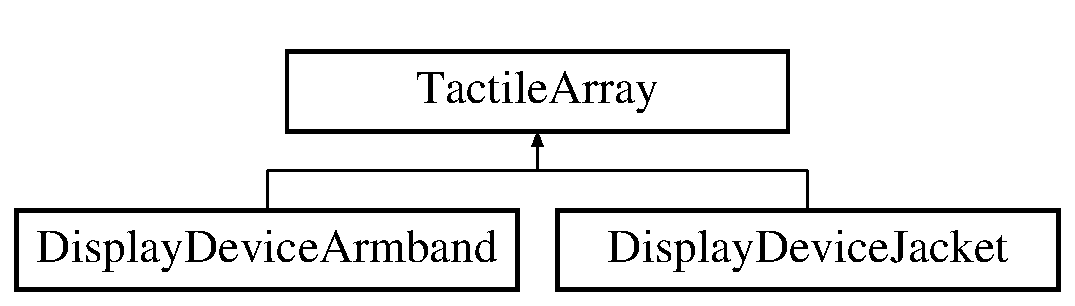
\includegraphics[height=2.000000cm]{classTactileArray}
\end{center}
\end{figure}
\subsection*{Public Member Functions}
\begin{DoxyCompactItemize}
\item 
\hypertarget{classTactileArray_acbfafee94d72b978ace17f08167fc036}{
{\bfseries TactileArray} (int a\_\-portNum)}
\label{classTactileArray_acbfafee94d72b978ace17f08167fc036}

\item 
\hypertarget{classTactileArray_aeadf3a68daab9c158a108a15debb28b8}{
bool {\bfseries openSerialPort} (int pNo=1, bool announce=false)}
\label{classTactileArray_aeadf3a68daab9c158a108a15debb28b8}

\item 
\hypertarget{classTactileArray_a3dd4969a067bd024a98fa9e99e40e971}{
bool {\bfseries closeSerialPort} ()}
\label{classTactileArray_a3dd4969a067bd024a98fa9e99e40e971}

\item 
\hypertarget{classTactileArray_ab8b3c1326d810855cde7422c93279dd1}{
bool {\bfseries initialize} (void)}
\label{classTactileArray_ab8b3c1326d810855cde7422c93279dd1}

\item 
\hypertarget{classTactileArray_afa6e34c93e1311edce551539831e0982}{
void {\bfseries setPort} (int a\_\-portNum)}
\label{classTactileArray_afa6e34c93e1311edce551539831e0982}

\item 
\hypertarget{classTactileArray_a62f715d4171c021a1d22ae67b2cb121d}{
void {\bfseries setIntensity} (int $\ast$pIntensityArray)}
\label{classTactileArray_a62f715d4171c021a1d22ae67b2cb121d}

\item 
\hypertarget{classTactileArray_a9d537a2423b2cba35badcca3468593f0}{
void {\bfseries setIntensity} (double $\ast$pIntensityArray)}
\label{classTactileArray_a9d537a2423b2cba35badcca3468593f0}

\item 
\hypertarget{classTactileArray_a57f15c2bbd18cbbdf2fe59d8a550d8a5}{
void {\bfseries setIntensity} (int arrayX, int arrayY, int intensity)}
\label{classTactileArray_a57f15c2bbd18cbbdf2fe59d8a550d8a5}

\item 
\hypertarget{classTactileArray_a8e84527dac8a4b36ac8dbddf50a4c855}{
void {\bfseries setIntensity} (int arrayX, int arrayY, double intensity)}
\label{classTactileArray_a8e84527dac8a4b36ac8dbddf50a4c855}

\item 
\hypertarget{classTactileArray_abbca9d69c0c6be1816214ebb75ecd16c}{
void {\bfseries setIntensityAll} (int intensity=0)}
\label{classTactileArray_abbca9d69c0c6be1816214ebb75ecd16c}

\item 
\hypertarget{classTactileArray_ad3edd3dc58c199e73a5095fe9ccb6c5e}{
void {\bfseries setIntensityAll} (double intensity)}
\label{classTactileArray_ad3edd3dc58c199e73a5095fe9ccb6c5e}

\item 
\hypertarget{classTactileArray_adc94914edaa38a6c261f2b8a42f88bbb}{
void {\bfseries setArraySize} (int a\_\-arraySizeX, int a\_\-arraySizeY)}
\label{classTactileArray_adc94914edaa38a6c261f2b8a42f88bbb}

\item 
\hypertarget{classTactileArray_a2d2e28e36c7d0f166e06d5061ba85196}{
void {\bfseries actuate} (void)}
\label{classTactileArray_a2d2e28e36c7d0f166e06d5061ba85196}

\item 
\hypertarget{classTactileArray_a40a5564388ad4ee3fabf8b9866538b48}{
void {\bfseries test1by1} (void)}
\label{classTactileArray_a40a5564388ad4ee3fabf8b9866538b48}

\item 
\hypertarget{classTactileArray_a5bb334c3d9bca1949141f7ae4a6637ba}{
int {\bfseries getMaxIntensity} (void) const }
\label{classTactileArray_a5bb334c3d9bca1949141f7ae4a6637ba}

\item 
\hypertarget{classTactileArray_a7a573669d558b1a22bf3e943795af119}{
int {\bfseries getArraySizeX} (void) const }
\label{classTactileArray_a7a573669d558b1a22bf3e943795af119}

\item 
\hypertarget{classTactileArray_a7dbe69bda14b3c208d96f4e5e1fa19be}{
int {\bfseries getArraySizeY} (void) const }
\label{classTactileArray_a7dbe69bda14b3c208d96f4e5e1fa19be}

\item 
\hypertarget{classTactileArray_afffd3159074b989045c47807b133cbec}{
int {\bfseries getArraySize} (void) const }
\label{classTactileArray_afffd3159074b989045c47807b133cbec}

\end{DoxyCompactItemize}


The documentation for this class was generated from the following files:\begin{DoxyCompactItemize}
\item 
/home/kevin/workspace/HugMe/HugMe v0.9.1/Jacket/TactileArray.h\item 
/home/kevin/workspace/HugMe/HugMe v0.9.1/Jacket/TactileArray.cpp\end{DoxyCompactItemize}

\hypertarget{classTDVCameraInterfaceBase}{
\section{TDVCameraInterfaceBase Class Reference}
\label{classTDVCameraInterfaceBase}\index{TDVCameraInterfaceBase@{TDVCameraInterfaceBase}}
}
Inheritance diagram for TDVCameraInterfaceBase:\begin{figure}[H]
\begin{center}
\leavevmode
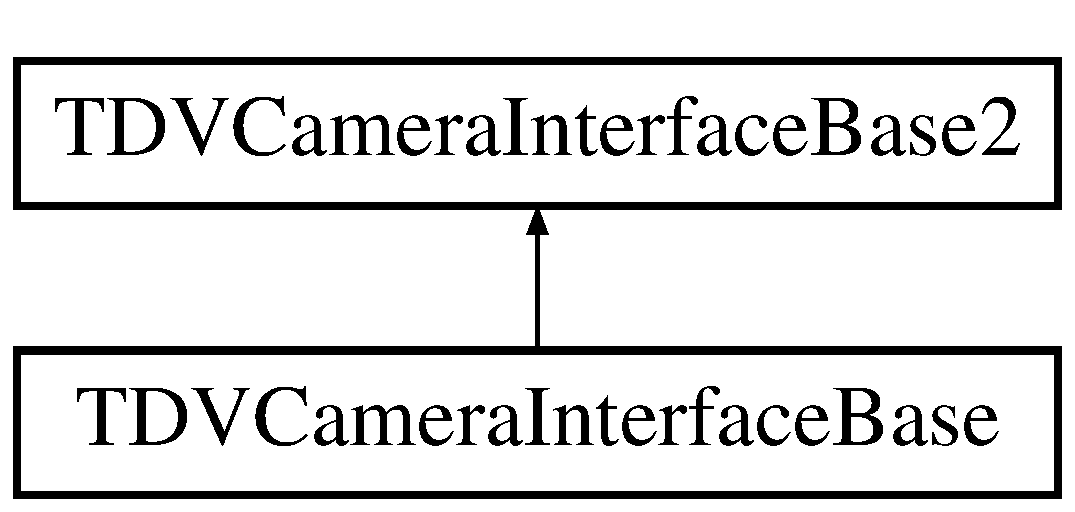
\includegraphics[height=2cm]{classTDVCameraInterfaceBase}
\end{center}
\end{figure}
\subsection*{Public Member Functions}
\begin{DoxyCompactItemize}
\item 
\hypertarget{classTDVCameraInterfaceBase_ae9e01cf3dc1a73620a056cc34586898a}{
bool {\bfseries isVideoActive} () const }
\label{classTDVCameraInterfaceBase_ae9e01cf3dc1a73620a056cc34586898a}

\item 
\hypertarget{classTDVCameraInterfaceBase_a21f0b98fc8fe110fa69de4f4d766a488}{
bool {\bfseries isCommActive} () const }
\label{classTDVCameraInterfaceBase_a21f0b98fc8fe110fa69de4f4d766a488}

\item 
\hypertarget{classTDVCameraInterfaceBase_ae371fdab81d2896f4d725a62c4157f5f}{
void {\bfseries setVideoCallBack} (videoCallBackFunc videoCBF, void $\ast$pObject=0)}
\label{classTDVCameraInterfaceBase_ae371fdab81d2896f4d725a62c4157f5f}

\item 
\hypertarget{classTDVCameraInterfaceBase_aecf920692d98daac41e09f597e1d32d5}{
void {\bfseries setCommandCallBack} (cmdCallBackFunc cmdCBF, void $\ast$pObject=0)}
\label{classTDVCameraInterfaceBase_aecf920692d98daac41e09f597e1d32d5}

\item 
\hypertarget{classTDVCameraInterfaceBase_aab7ffba266ac2d0c1a20694cab5953e7}{
bool {\bfseries getVideoSize} (int \&width, int \&height, int \&rgbPixelSize, int \&depthPixelSize) const }
\label{classTDVCameraInterfaceBase_aab7ffba266ac2d0c1a20694cab5953e7}

\item 
\hypertarget{classTDVCameraInterfaceBase_a6338dae33c7e3c4184161944832e9d99}{
bool {\bfseries getRGBFullResSize} (int \&width, int \&height, int \&rgbPixelSize)}
\label{classTDVCameraInterfaceBase_a6338dae33c7e3c4184161944832e9d99}

\item 
\hypertarget{classTDVCameraInterfaceBase_abc48f94311e7aadf0c6a0df157951097}{
virtual HRESULT {\bfseries setCameraCommand} (int cmdID, int value)}
\label{classTDVCameraInterfaceBase_abc48f94311e7aadf0c6a0df157951097}

\item 
\hypertarget{classTDVCameraInterfaceBase_a136acd03b9cf0e8ee17af7679721d82a}{
virtual HRESULT {\bfseries getCameraCommandVal} (int cmdID, int \&value) const }
\label{classTDVCameraInterfaceBase_a136acd03b9cf0e8ee17af7679721d82a}

\item 
\hypertarget{classTDVCameraInterfaceBase_a8734112fa15f5cfe893a9aab872cf12a}{
virtual HRESULT {\bfseries getCameraCommandLimits} (int cmdID, int \&minValue, int \&maxValue) const }
\label{classTDVCameraInterfaceBase_a8734112fa15f5cfe893a9aab872cf12a}

\item 
\hypertarget{classTDVCameraInterfaceBase_a38695ddb9698f59037add68798257aac}{
virtual HRESULT {\bfseries getVideoBuffer} (int bufferType, unsigned char $\ast$\&pBuffer)}
\label{classTDVCameraInterfaceBase_a38695ddb9698f59037add68798257aac}

\item 
\hypertarget{classTDVCameraInterfaceBase_a5cdbb3ec301333c9c573fb58b50683b1}{
void {\bfseries SetMaintenanceCmd} (int ID, int val)}
\label{classTDVCameraInterfaceBase_a5cdbb3ec301333c9c573fb58b50683b1}

\end{DoxyCompactItemize}


The documentation for this class was generated from the following file:\begin{DoxyCompactItemize}
\item 
/home/kevin/workspace/HugMe/HugMe v0.9.1/ZCamera/TDVCameraInterface.h\end{DoxyCompactItemize}

\hypertarget{classTDVCameraInterfaceBase2}{
\section{TDVCameraInterfaceBase2 Class Reference}
\label{classTDVCameraInterfaceBase2}\index{TDVCameraInterfaceBase2@{TDVCameraInterfaceBase2}}
}
Inheritance diagram for TDVCameraInterfaceBase2:\begin{figure}[H]
\begin{center}
\leavevmode
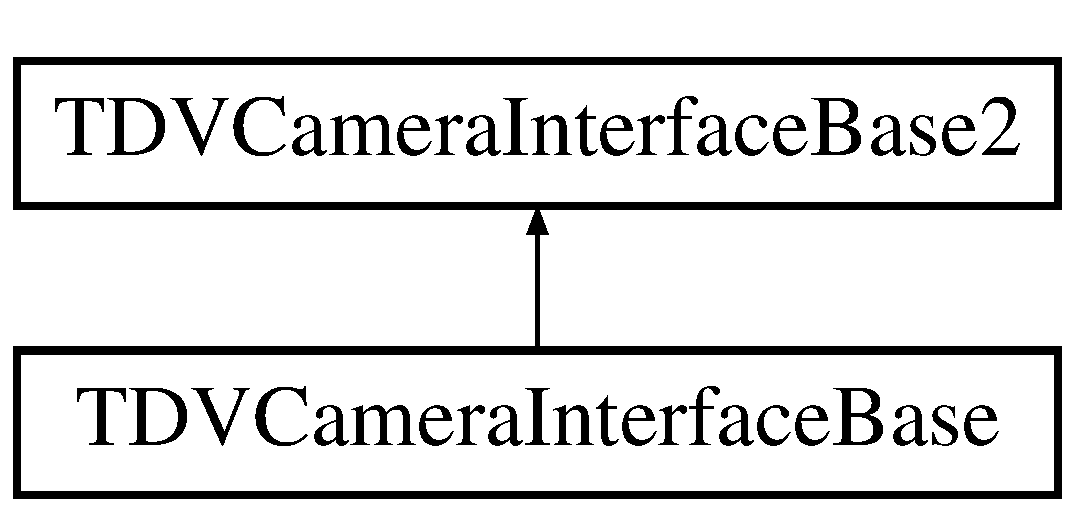
\includegraphics[height=2.000000cm]{classTDVCameraInterfaceBase2}
\end{center}
\end{figure}
\subsection*{Public Member Functions}
\begin{DoxyCompactItemize}
\item 
\hypertarget{classTDVCameraInterfaceBase2_a684145d3ee389c45eb5677eab1e55759}{
virtual HRESULT {\bfseries setCameraCommand} (int cmdID, int value)=0}
\label{classTDVCameraInterfaceBase2_a684145d3ee389c45eb5677eab1e55759}

\item 
\hypertarget{classTDVCameraInterfaceBase2_ab6322af8ebc298d65d06b5194441e43b}{
virtual HRESULT {\bfseries getCameraCommandVal} (int cmdID, int \&value) const =0}
\label{classTDVCameraInterfaceBase2_ab6322af8ebc298d65d06b5194441e43b}

\item 
\hypertarget{classTDVCameraInterfaceBase2_a3019b4da3230741db16d122ac7980503}{
virtual HRESULT {\bfseries getCameraCommandLimits} (int cmdID, int \&minValue, int \&maxValue) const =0}
\label{classTDVCameraInterfaceBase2_a3019b4da3230741db16d122ac7980503}

\item 
\hypertarget{classTDVCameraInterfaceBase2_a51410aae9341c6809bedea5c79091d82}{
virtual HRESULT {\bfseries getVideoBuffer} (int bufferType, unsigned char $\ast$\&pBuffer)=0}
\label{classTDVCameraInterfaceBase2_a51410aae9341c6809bedea5c79091d82}

\item 
\hypertarget{classTDVCameraInterfaceBase2_a54e310f7c97367f393a05439b260bc05}{
void {\bfseries cmdColorCameraSetting} (int iColorCommandID, int iValue)}
\label{classTDVCameraInterfaceBase2_a54e310f7c97367f393a05439b260bc05}

\item 
\hypertarget{classTDVCameraInterfaceBase2_a63c1f5ddf8b9af6e7b8b156088c5f789}{
bool {\bfseries getColorCameraSetting} (int iColorCommandID, int \&iValue) const }
\label{classTDVCameraInterfaceBase2_a63c1f5ddf8b9af6e7b8b156088c5f789}

\item 
\hypertarget{classTDVCameraInterfaceBase2_af269978a958edc2dc7baea5bc5bcdef6}{
bool {\bfseries getColorCameraSettingLimit} (int iColorCommandID, int \&min, int \&max) const }
\label{classTDVCameraInterfaceBase2_af269978a958edc2dc7baea5bc5bcdef6}

\item 
\hypertarget{classTDVCameraInterfaceBase2_a8c02c4da359f4e0125c7065819d1e8c7}{
void {\bfseries cmdCameraOn} ()}
\label{classTDVCameraInterfaceBase2_a8c02c4da359f4e0125c7065819d1e8c7}

\item 
\hypertarget{classTDVCameraInterfaceBase2_a6c7e30c193de170600f89a9d057412f7}{
void {\bfseries cmdCameraOff} ()}
\label{classTDVCameraInterfaceBase2_a6c7e30c193de170600f89a9d057412f7}

\item 
\hypertarget{classTDVCameraInterfaceBase2_a988c6da99531b00c8071b9869748417b}{
bool {\bfseries isCameraOn} () const }
\label{classTDVCameraInterfaceBase2_a988c6da99531b00c8071b9869748417b}

\item 
\hypertarget{classTDVCameraInterfaceBase2_aa7e00476c05bf11c55016d2e3923ba5a}{
int {\bfseries getMaxBrightness} () const }
\label{classTDVCameraInterfaceBase2_aa7e00476c05bf11c55016d2e3923ba5a}

\item 
\hypertarget{classTDVCameraInterfaceBase2_aab905160ffcd2009c6a90aacd95301a2}{
int {\bfseries getMinBrightness} () const }
\label{classTDVCameraInterfaceBase2_aab905160ffcd2009c6a90aacd95301a2}

\item 
\hypertarget{classTDVCameraInterfaceBase2_ab343a20c0bb19fe8ae30bab85d401baa}{
void {\bfseries cmdPrimaryBrightness} (int value)}
\label{classTDVCameraInterfaceBase2_ab343a20c0bb19fe8ae30bab85d401baa}

\item 
\hypertarget{classTDVCameraInterfaceBase2_aa616448268d8472c195278ac9b3aee0b}{
int {\bfseries getPrimaryBrightness} () const }
\label{classTDVCameraInterfaceBase2_aa616448268d8472c195278ac9b3aee0b}

\item 
\hypertarget{classTDVCameraInterfaceBase2_ae5c5e7f25aca037e483ac1236d58fe5f}{
void {\bfseries cmdSecondaryBrightness} (int value)}
\label{classTDVCameraInterfaceBase2_ae5c5e7f25aca037e483ac1236d58fe5f}

\item 
\hypertarget{classTDVCameraInterfaceBase2_aa0bf4daab59df0e592768a68cfab8c43}{
int {\bfseries getSecondaryBrightness} () const }
\label{classTDVCameraInterfaceBase2_aa0bf4daab59df0e592768a68cfab8c43}

\item 
\hypertarget{classTDVCameraInterfaceBase2_a63ac302b5a4e2f27b66ba08f11911f70}{
int {\bfseries getMaxWidth} () const }
\label{classTDVCameraInterfaceBase2_a63ac302b5a4e2f27b66ba08f11911f70}

\item 
\hypertarget{classTDVCameraInterfaceBase2_acfc463b8b3f949de11b589fed48638a6}{
int {\bfseries getMinWidth} () const }
\label{classTDVCameraInterfaceBase2_acfc463b8b3f949de11b589fed48638a6}

\item 
\hypertarget{classTDVCameraInterfaceBase2_a7c11a0dfa3230006f7b870dd9f5c950c}{
void {\bfseries cmdPrimaryWidth} (int value)}
\label{classTDVCameraInterfaceBase2_a7c11a0dfa3230006f7b870dd9f5c950c}

\item 
\hypertarget{classTDVCameraInterfaceBase2_a714dd64055e8ecdf851f5cdc8c899c25}{
int {\bfseries getPrimaryWidth} () const }
\label{classTDVCameraInterfaceBase2_a714dd64055e8ecdf851f5cdc8c899c25}

\item 
\hypertarget{classTDVCameraInterfaceBase2_a5062371499a5f5fa262f8fef22efdfc9}{
void {\bfseries cmdSecondaryWidth} (int value)}
\label{classTDVCameraInterfaceBase2_a5062371499a5f5fa262f8fef22efdfc9}

\item 
\hypertarget{classTDVCameraInterfaceBase2_a52828a04c73328758d67b6f381653428}{
int {\bfseries getSecondaryWidth} () const }
\label{classTDVCameraInterfaceBase2_a52828a04c73328758d67b6f381653428}

\item 
\hypertarget{classTDVCameraInterfaceBase2_ad7b72ddc0bdac856e4dc5fb6bbb99cfc}{
int {\bfseries getMaxDistance} () const }
\label{classTDVCameraInterfaceBase2_ad7b72ddc0bdac856e4dc5fb6bbb99cfc}

\item 
\hypertarget{classTDVCameraInterfaceBase2_ac87c6734afdc4dd27cf37d7d92d128ab}{
int {\bfseries getMinDistance} () const }
\label{classTDVCameraInterfaceBase2_ac87c6734afdc4dd27cf37d7d92d128ab}

\item 
\hypertarget{classTDVCameraInterfaceBase2_a60fad90a7ebd5354ccca87e19abdfd28}{
void {\bfseries cmdPrimaryDist} (int value)}
\label{classTDVCameraInterfaceBase2_a60fad90a7ebd5354ccca87e19abdfd28}

\item 
\hypertarget{classTDVCameraInterfaceBase2_aea0a3141dae5b18e66b81862be286e90}{
int {\bfseries getPrimaryDist} () const }
\label{classTDVCameraInterfaceBase2_aea0a3141dae5b18e66b81862be286e90}

\item 
\hypertarget{classTDVCameraInterfaceBase2_a711d6c76704fb19d4cf17612a131ed18}{
void {\bfseries cmdSecondaryDist} (int value)}
\label{classTDVCameraInterfaceBase2_a711d6c76704fb19d4cf17612a131ed18}

\item 
\hypertarget{classTDVCameraInterfaceBase2_acfa0c0769263b2852ffb7893cff1179e}{
int {\bfseries getSecondaryDist} () const }
\label{classTDVCameraInterfaceBase2_acfa0c0769263b2852ffb7893cff1179e}

\item 
\hypertarget{classTDVCameraInterfaceBase2_a91c347ac98df9fce1bdae10ac0988d5b}{
int {\bfseries getMaxGain} () const }
\label{classTDVCameraInterfaceBase2_a91c347ac98df9fce1bdae10ac0988d5b}

\item 
\hypertarget{classTDVCameraInterfaceBase2_a2ebfb11b935fac730c9aa973a67e2bac}{
int {\bfseries getMinGain} () const }
\label{classTDVCameraInterfaceBase2_a2ebfb11b935fac730c9aa973a67e2bac}

\item 
\hypertarget{classTDVCameraInterfaceBase2_ac7cd647d5f8ea76b305c0ba4d434acd4}{
void {\bfseries cmdGain} (int value)}
\label{classTDVCameraInterfaceBase2_ac7cd647d5f8ea76b305c0ba4d434acd4}

\item 
\hypertarget{classTDVCameraInterfaceBase2_a78a534aa9676766be2338ef68302e640}{
int {\bfseries getGain} () const }
\label{classTDVCameraInterfaceBase2_a78a534aa9676766be2338ef68302e640}

\item 
\hypertarget{classTDVCameraInterfaceBase2_aafed77798e0cf7c8e2c5093782a16361}{
int {\bfseries getMinFilterVal} () const }
\label{classTDVCameraInterfaceBase2_aafed77798e0cf7c8e2c5093782a16361}

\item 
\hypertarget{classTDVCameraInterfaceBase2_acc7400a53f77b2c5d94aed93009579b7}{
int {\bfseries getMaxFilterVal} () const }
\label{classTDVCameraInterfaceBase2_acc7400a53f77b2c5d94aed93009579b7}

\item 
\hypertarget{classTDVCameraInterfaceBase2_a153203745fb70783b166d29935d05adf}{
int {\bfseries getMinSoftnessVal} () const }
\label{classTDVCameraInterfaceBase2_a153203745fb70783b166d29935d05adf}

\item 
\hypertarget{classTDVCameraInterfaceBase2_a177b2e039f3abdb3a8b75f9f41c7d78d}{
int {\bfseries getMaxSoftnessVal} () const }
\label{classTDVCameraInterfaceBase2_a177b2e039f3abdb3a8b75f9f41c7d78d}

\item 
\hypertarget{classTDVCameraInterfaceBase2_aa76b67341fee260a64c81419125822b0}{
void {\bfseries cmdBinVal} (int value)}
\label{classTDVCameraInterfaceBase2_aa76b67341fee260a64c81419125822b0}

\item 
\hypertarget{classTDVCameraInterfaceBase2_a306c0eda9013f9236de4bfc77d75d011}{
int {\bfseries getBinVal} () const }
\label{classTDVCameraInterfaceBase2_a306c0eda9013f9236de4bfc77d75d011}

\item 
\hypertarget{classTDVCameraInterfaceBase2_a0e4ca14432e810b4d0c44da6d41371ac}{
void {\bfseries cmdBinarizeOnOff} (bool value)}
\label{classTDVCameraInterfaceBase2_a0e4ca14432e810b4d0c44da6d41371ac}

\item 
\hypertarget{classTDVCameraInterfaceBase2_a0f313e34b1e754bfefa21cbccd4d914c}{
bool {\bfseries getBinarizeOnOff} () const }
\label{classTDVCameraInterfaceBase2_a0f313e34b1e754bfefa21cbccd4d914c}

\item 
\hypertarget{classTDVCameraInterfaceBase2_a7565271a8464c7de45e470218b19f2fc}{
void {\bfseries cmdMedianOnOff} (bool value)}
\label{classTDVCameraInterfaceBase2_a7565271a8464c7de45e470218b19f2fc}

\item 
\hypertarget{classTDVCameraInterfaceBase2_a209bf23c6415591265b1fa9655f9be0a}{
bool {\bfseries getMedianOnOff} () const }
\label{classTDVCameraInterfaceBase2_a209bf23c6415591265b1fa9655f9be0a}

\item 
\hypertarget{classTDVCameraInterfaceBase2_a5424cfc75464477533219db9407f1810}{
void {\bfseries cmdInvertOnOff} (bool value)}
\label{classTDVCameraInterfaceBase2_a5424cfc75464477533219db9407f1810}

\item 
\hypertarget{classTDVCameraInterfaceBase2_a1e5ef180ec2dcbc7dafdcf536c4b907f}{
bool {\bfseries getInvertOnOff} () const }
\label{classTDVCameraInterfaceBase2_a1e5ef180ec2dcbc7dafdcf536c4b907f}

\item 
\hypertarget{classTDVCameraInterfaceBase2_a25480b123cc8ea96b76055d47fef3705}{
void {\bfseries cmdTemporalFilterOnOff} (bool value)}
\label{classTDVCameraInterfaceBase2_a25480b123cc8ea96b76055d47fef3705}

\item 
\hypertarget{classTDVCameraInterfaceBase2_a4aba5abd0c3f72115d4d84ab42bff89b}{
bool {\bfseries getTemporalFilterOnOff} () const }
\label{classTDVCameraInterfaceBase2_a4aba5abd0c3f72115d4d84ab42bff89b}

\item 
\hypertarget{classTDVCameraInterfaceBase2_aee223c818363239f0b7308b589a676b5}{
void {\bfseries cmdSmoothOnOff} (bool value)}
\label{classTDVCameraInterfaceBase2_aee223c818363239f0b7308b589a676b5}

\item 
\hypertarget{classTDVCameraInterfaceBase2_a489f0ed0b9bbd69b259e5f08f96f1cb8}{
bool {\bfseries getSmoothOnOff} () const }
\label{classTDVCameraInterfaceBase2_a489f0ed0b9bbd69b259e5f08f96f1cb8}

\item 
\hypertarget{classTDVCameraInterfaceBase2_ab1d2c9cc2676b858c0dbf50035ee36f4}{
void {\bfseries cmdSoftness} (int value)}
\label{classTDVCameraInterfaceBase2_ab1d2c9cc2676b858c0dbf50035ee36f4}

\item 
\hypertarget{classTDVCameraInterfaceBase2_a3cc4d16af60928ede441533b47792db0}{
int {\bfseries getSoftness} () const }
\label{classTDVCameraInterfaceBase2_a3cc4d16af60928ede441533b47792db0}

\item 
\hypertarget{classTDVCameraInterfaceBase2_a278bad41877f7cc67010513edddcb371}{
void {\bfseries cmdMaskSmoothOnOff} (bool value)}
\label{classTDVCameraInterfaceBase2_a278bad41877f7cc67010513edddcb371}

\item 
\hypertarget{classTDVCameraInterfaceBase2_a5a643241c1c220a61ecf0c0a22e58229}{
bool {\bfseries getMaskSmoothOnOff} () const }
\label{classTDVCameraInterfaceBase2_a5a643241c1c220a61ecf0c0a22e58229}

\item 
\hypertarget{classTDVCameraInterfaceBase2_a7fd8c3ef57e1a603d8341e1b8f605d82}{
void {\bfseries cmdMaskSoftness} (int value)}
\label{classTDVCameraInterfaceBase2_a7fd8c3ef57e1a603d8341e1b8f605d82}

\item 
\hypertarget{classTDVCameraInterfaceBase2_aa9e8296220d1f6dfd0b3e80b186ce2fc}{
int {\bfseries getMaskSoftness} () const }
\label{classTDVCameraInterfaceBase2_aa9e8296220d1f6dfd0b3e80b186ce2fc}

\item 
\hypertarget{classTDVCameraInterfaceBase2_a79660c40a44100ab0162dc1691d742ad}{
void {\bfseries cmdAutomaticBackgroundOnOff} (bool value)}
\label{classTDVCameraInterfaceBase2_a79660c40a44100ab0162dc1691d742ad}

\item 
\hypertarget{classTDVCameraInterfaceBase2_a06af73ceaff68f12f4854ba1eb529c08}{
bool {\bfseries getAutomaticBackground} ()}
\label{classTDVCameraInterfaceBase2_a06af73ceaff68f12f4854ba1eb529c08}

\item 
\hypertarget{classTDVCameraInterfaceBase2_a4267605549783aba6499aa07cf35f3d1}{
void {\bfseries cmdAutomaticDepthPositionOnOff} (bool value)}
\label{classTDVCameraInterfaceBase2_a4267605549783aba6499aa07cf35f3d1}

\item 
\hypertarget{classTDVCameraInterfaceBase2_a854c8f778aa3f13c66c2639b5905e428}{
bool {\bfseries getAutomaticDepthPosition} ()}
\label{classTDVCameraInterfaceBase2_a854c8f778aa3f13c66c2639b5905e428}

\item 
\hypertarget{classTDVCameraInterfaceBase2_a941bef4b230eabf386507dca5299ecff}{
void {\bfseries cmdClean} (int value)}
\label{classTDVCameraInterfaceBase2_a941bef4b230eabf386507dca5299ecff}

\item 
\hypertarget{classTDVCameraInterfaceBase2_a56a29cde8078bcc26ce736a104a46ecc}{
int {\bfseries getClean} () const }
\label{classTDVCameraInterfaceBase2_a56a29cde8078bcc26ce736a104a46ecc}

\item 
\hypertarget{classTDVCameraInterfaceBase2_acae599e652152613bcfaab6334349471}{
bool {\bfseries cmdSaveStatus} (int index)}
\label{classTDVCameraInterfaceBase2_acae599e652152613bcfaab6334349471}

\item 
\hypertarget{classTDVCameraInterfaceBase2_a2a676dabbdbd67950e3cb764d97207f4}{
bool {\bfseries cmdRestoreStatus} (int index)}
\label{classTDVCameraInterfaceBase2_a2a676dabbdbd67950e3cb764d97207f4}

\item 
\hypertarget{classTDVCameraInterfaceBase2_a9479b1f2083c5135bc4ed758f87eb826}{
void {\bfseries cmdStartAutomaticFind} ()}
\label{classTDVCameraInterfaceBase2_a9479b1f2083c5135bc4ed758f87eb826}

\item 
\hypertarget{classTDVCameraInterfaceBase2_ab2d29930d4ddbaf855e43ccaa139c4c2}{
bool {\bfseries isDuringAutomaticFind} () const }
\label{classTDVCameraInterfaceBase2_ab2d29930d4ddbaf855e43ccaa139c4c2}

\item 
\hypertarget{classTDVCameraInterfaceBase2_a88da987cea5ee76654e64525c2938c57}{
void {\bfseries cmdAutomaticTracking} (bool state)}
\label{classTDVCameraInterfaceBase2_a88da987cea5ee76654e64525c2938c57}

\item 
\hypertarget{classTDVCameraInterfaceBase2_a248c84bbb1232285fa00069d6263e8c7}{
bool {\bfseries isAutomaticTrackingOn} () const }
\label{classTDVCameraInterfaceBase2_a248c84bbb1232285fa00069d6263e8c7}

\item 
\hypertarget{classTDVCameraInterfaceBase2_ab0839cd442d3a1c47b7c55578cf7ab0a}{
void {\bfseries cmdAutomaticBrightness} (bool state)}
\label{classTDVCameraInterfaceBase2_ab0839cd442d3a1c47b7c55578cf7ab0a}

\item 
\hypertarget{classTDVCameraInterfaceBase2_a54c95ac82e08bb3a2ee0ef847af2fd8d}{
bool {\bfseries isAutomaticBrightnessOn} () const }
\label{classTDVCameraInterfaceBase2_a54c95ac82e08bb3a2ee0ef847af2fd8d}

\item 
\hypertarget{classTDVCameraInterfaceBase2_ab1bfb1c5500793508cbe2c1c7d8d9a2b}{
void {\bfseries cmdSaveImage} ()}
\label{classTDVCameraInterfaceBase2_ab1bfb1c5500793508cbe2c1c7d8d9a2b}

\item 
\hypertarget{classTDVCameraInterfaceBase2_a528e6c9ab7b284456571e5c954e0663a}{
void {\bfseries cmdSaveImageAverage} ()}
\label{classTDVCameraInterfaceBase2_a528e6c9ab7b284456571e5c954e0663a}

\item 
\hypertarget{classTDVCameraInterfaceBase2_a7efb94988412cbb758d3b8971f4463a9}{
void {\bfseries cmdSaveSequence} (int length, bool saveAVI)}
\label{classTDVCameraInterfaceBase2_a7efb94988412cbb758d3b8971f4463a9}

\item 
\hypertarget{classTDVCameraInterfaceBase2_aa2705a831908bb92aea85cb3cde82854}{
void {\bfseries cmdVideoFreeze} (bool state, bool useAverage=false)}
\label{classTDVCameraInterfaceBase2_aa2705a831908bb92aea85cb3cde82854}

\item 
\hypertarget{classTDVCameraInterfaceBase2_a649b5e579d9f165c3fd08ca224bac40a}{
void {\bfseries cmdRGBProcessing} (bool status)}
\label{classTDVCameraInterfaceBase2_a649b5e579d9f165c3fd08ca224bac40a}

\item 
\hypertarget{classTDVCameraInterfaceBase2_a662d62abb6a0b268e9fe95fd545c360c}{
bool {\bfseries getRGBProcessing} () const }
\label{classTDVCameraInterfaceBase2_a662d62abb6a0b268e9fe95fd545c360c}

\item 
\hypertarget{classTDVCameraInterfaceBase2_a6f2b9e9efbbaddfc80801ab5cd0a99f1}{
void {\bfseries cmdConfidenceMapProcessing} (bool status)}
\label{classTDVCameraInterfaceBase2_a6f2b9e9efbbaddfc80801ab5cd0a99f1}

\item 
\hypertarget{classTDVCameraInterfaceBase2_a326817d66da92c7f7b022d8460097019}{
bool {\bfseries getConfidenceMapProcessing} () const }
\label{classTDVCameraInterfaceBase2_a326817d66da92c7f7b022d8460097019}

\item 
\hypertarget{classTDVCameraInterfaceBase2_ab1bea9c049e62e010f0f62a168bc30d2}{
void {\bfseries cmdIRTransfer} (bool status)}
\label{classTDVCameraInterfaceBase2_ab1bea9c049e62e010f0f62a168bc30d2}

\item 
\hypertarget{classTDVCameraInterfaceBase2_ab3f3b322e7216a5222306e1fc2debcbe}{
bool {\bfseries getIRTransfer} () const }
\label{classTDVCameraInterfaceBase2_ab3f3b322e7216a5222306e1fc2debcbe}

\item 
\hypertarget{classTDVCameraInterfaceBase2_a8030d68df7c717b78af36d151cdf618f}{
void {\bfseries cmdRGBFullRes} (bool status)}
\label{classTDVCameraInterfaceBase2_a8030d68df7c717b78af36d151cdf618f}

\item 
\hypertarget{classTDVCameraInterfaceBase2_a49c8dd40ebb60cf565b6163dae3c5777}{
bool {\bfseries getRGBFullRes} () const }
\label{classTDVCameraInterfaceBase2_a49c8dd40ebb60cf565b6163dae3c5777}

\item 
\hypertarget{classTDVCameraInterfaceBase2_a41bafb7ada57dd229420462eb74e7e9a}{
bool {\bfseries getConfidenceFrame} (unsigned char $\ast$\&pConfidence)}
\label{classTDVCameraInterfaceBase2_a41bafb7ada57dd229420462eb74e7e9a}

\item 
\hypertarget{classTDVCameraInterfaceBase2_ad7be19b42aa545d68a03b742105fa5fd}{
bool {\bfseries getSourceIRFrames} (unsigned char $\ast$\&pPrimary, unsigned char $\ast$\&pSecondary)}
\label{classTDVCameraInterfaceBase2_ad7be19b42aa545d68a03b742105fa5fd}

\item 
\hypertarget{classTDVCameraInterfaceBase2_a559c0138bfc30147bdadbc765caa3e54}{
bool {\bfseries getRGBFullResolutionFrame} (unsigned char $\ast$\&pRGBFullRes)}
\label{classTDVCameraInterfaceBase2_a559c0138bfc30147bdadbc765caa3e54}

\end{DoxyCompactItemize}


The documentation for this class was generated from the following file:\begin{DoxyCompactItemize}
\item 
/home/kevin/workspace/HugMe/HugMe v0.9.1/ZCamera/TDVCameraInterface2.h\end{DoxyCompactItemize}

\hypertarget{classTestRunner}{
\section{TestRunner Class Reference}
\label{classTestRunner}\index{TestRunner@{TestRunner}}
}


This class is used to start all the unit tests.  




{\ttfamily \#include $<$TestRunner.h$>$}

\subsection*{Public Member Functions}
\begin{DoxyCompactItemize}
\item 
\hypertarget{classTestRunner_a692f0bb1327c4092398b95c27ec6957b}{
void {\bfseries run} ()}
\label{classTestRunner_a692f0bb1327c4092398b95c27ec6957b}

\item 
\hypertarget{classTestRunner_a5d3932d4614f12c9fca2870597b90e1d}{
void {\bfseries toStream} (std::ostream \&os) const }
\label{classTestRunner_a5d3932d4614f12c9fca2870597b90e1d}

\end{DoxyCompactItemize}


\subsection{Detailed Description}
This class is used to start all the unit tests. 

The documentation for this class was generated from the following files:\begin{DoxyCompactItemize}
\item 
/home/kevin/workspace/HugMe/HugMe v0.9.1/Test/TestRunner.h\item 
/home/kevin/workspace/HugMe/HugMe v0.9.1/Test/TestRunner.cpp\end{DoxyCompactItemize}

\hypertarget{classTitleScreen}{
\section{TitleScreen Class Reference}
\label{classTitleScreen}\index{TitleScreen@{TitleScreen}}
}


The title screen is a 3D environment that is displayed when the game isn't running.  




{\ttfamily \#include $<$TitleScreen.h$>$}

\subsection*{Public Member Functions}
\begin{DoxyCompactItemize}
\item 
\hypertarget{classTitleScreen_a7aa7add9040c34b655bcde4cd6e758f2}{
\hyperlink{classTitleScreen_a7aa7add9040c34b655bcde4cd6e758f2}{TitleScreen} ()}
\label{classTitleScreen_a7aa7add9040c34b655bcde4cd6e758f2}

\begin{DoxyCompactList}\small\item\em Constructor. \item\end{DoxyCompactList}\item 
\hypertarget{classTitleScreen_a4f844eb163acc5b2373f6330b37673c1}{
virtual \hyperlink{classTitleScreen_a4f844eb163acc5b2373f6330b37673c1}{$\sim$TitleScreen} ()}
\label{classTitleScreen_a4f844eb163acc5b2373f6330b37673c1}

\begin{DoxyCompactList}\small\item\em Destructor. \item\end{DoxyCompactList}\item 
cCamera $\ast$ \hyperlink{classTitleScreen_aafaa452d86899a0fa60405fa1b82754e}{camera} ()
\begin{DoxyCompactList}\small\item\em Retrieve the camera for this title screen. \item\end{DoxyCompactList}\end{DoxyCompactItemize}


\subsection{Detailed Description}
The title screen is a 3D environment that is displayed when the game isn't running. 

\subsection{Member Function Documentation}
\hypertarget{classTitleScreen_aafaa452d86899a0fa60405fa1b82754e}{
\index{TitleScreen@{TitleScreen}!camera@{camera}}
\index{camera@{camera}!TitleScreen@{TitleScreen}}
\subsubsection[{camera}]{\setlength{\rightskip}{0pt plus 5cm}cCamera $\ast$ TitleScreen::camera (
\begin{DoxyParamCaption}
{}
\end{DoxyParamCaption}
)}}
\label{classTitleScreen_aafaa452d86899a0fa60405fa1b82754e}


Retrieve the camera for this title screen. 

\begin{DoxyReturn}{Returns}
The camera that should be used to render this environment 
\end{DoxyReturn}


The documentation for this class was generated from the following files:\begin{DoxyCompactItemize}
\item 
/home/kevin/workspace/HugMe/HugMe v0.9.1/Game/TitleScreen.h\item 
/home/kevin/workspace/HugMe/HugMe v0.9.1/Game/TitleScreen.cpp\end{DoxyCompactItemize}

\hypertarget{classUserInterface}{
\section{UserInterface Class Reference}
\label{classUserInterface}\index{UserInterface@{UserInterface}}
}
Inheritance diagram for UserInterface:\begin{figure}[H]
\begin{center}
\leavevmode
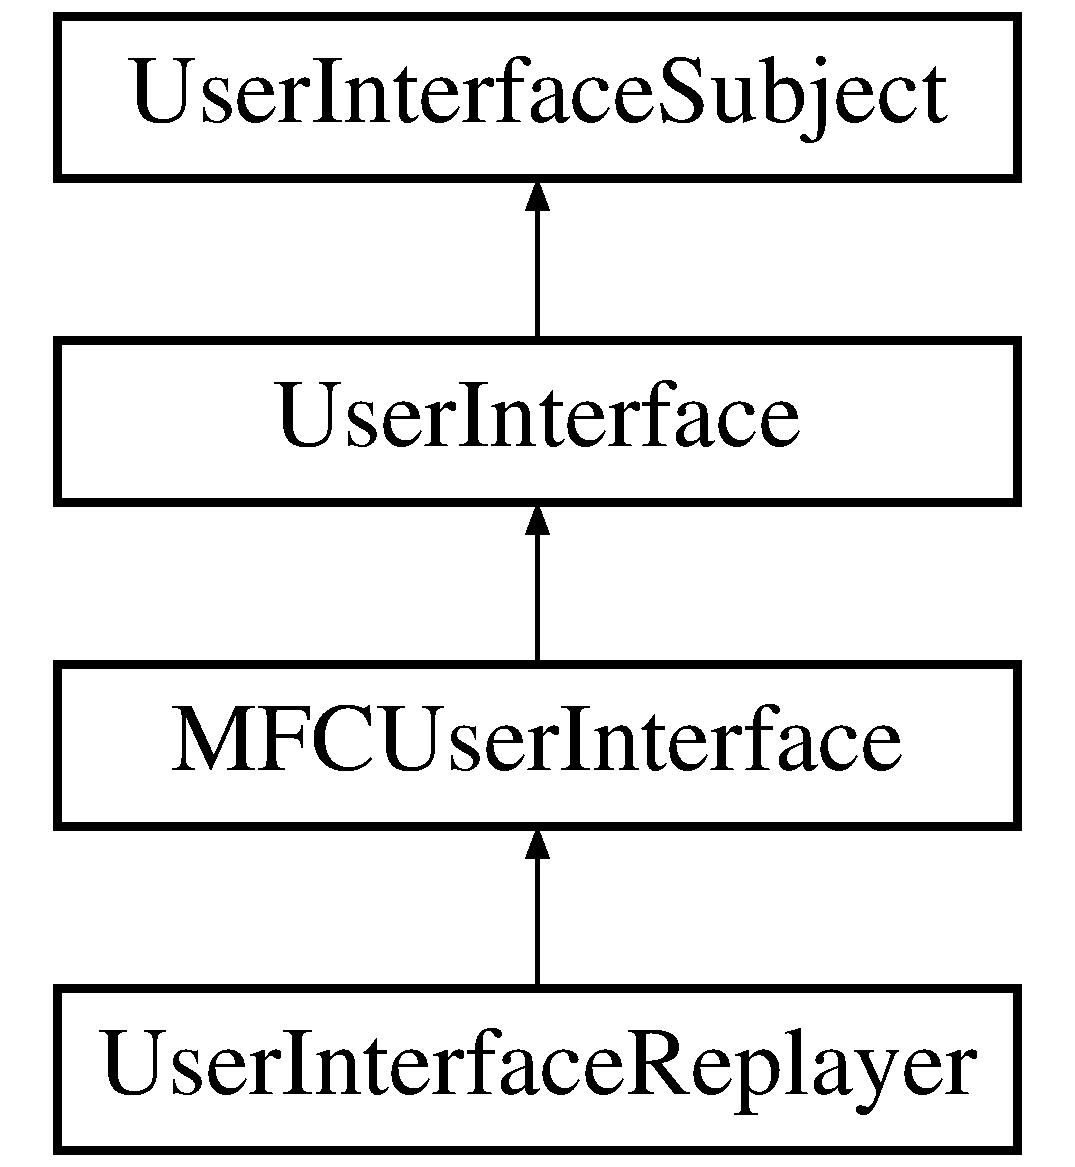
\includegraphics[height=4.000000cm]{classUserInterface}
\end{center}
\end{figure}
\subsection*{Public Member Functions}
\begin{DoxyCompactItemize}
\item 
virtual void \hyperlink{classUserInterface_ac43bf70dfea5b28e4cc185a0a72334c3}{switchCamera} (cCamera $\ast$camera)=0
\begin{DoxyCompactList}\small\item\em Changes the camera from which the vritual world will be displayed. \item\end{DoxyCompactList}\item 
\hypertarget{classUserInterface_a80c9af3149653a9fcca77994ff921520}{
virtual void {\bfseries displayConnectionStateChanged} (\hyperlink{namespaceConnectionState_ad1b6674b6f1c58f17e9db75d0a77149f}{ConnectionState\_\-t} state, \hyperlink{namespacePlayer_acc4ced29e6b7e20f602b3c8b60c75228}{Player\_\-t} player)=0}
\label{classUserInterface_a80c9af3149653a9fcca77994ff921520}

\item 
\hypertarget{classUserInterface_aea6b02914ae2d7ffe561189d7c7c7802}{
virtual void {\bfseries displayGameStateChanged} (\hyperlink{namespaceGameState_a1026e99904938017415f188e2daba514}{GameState\_\-t} state, \hyperlink{namespacePlayer_acc4ced29e6b7e20f602b3c8b60c75228}{Player\_\-t} player)=0}
\label{classUserInterface_aea6b02914ae2d7ffe561189d7c7c7802}

\item 
\hypertarget{classUserInterface_aa5d1fd621af37b9d57269ea57ea1470a}{
virtual void {\bfseries displayConnectionFailed} ()=0}
\label{classUserInterface_aa5d1fd621af37b9d57269ea57ea1470a}

\item 
\hypertarget{classUserInterface_a62d5eb6ee2406546e588dcd640e50b9d}{
virtual void {\bfseries displayFailedToListen} ()=0}
\label{classUserInterface_a62d5eb6ee2406546e588dcd640e50b9d}

\item 
\hypertarget{classUserInterface_a4dfc4010db770d8be0a7a9dd4d9eaa98}{
virtual void {\bfseries displayNetworkError} ()=0}
\label{classUserInterface_a4dfc4010db770d8be0a7a9dd4d9eaa98}

\item 
\hypertarget{classUserInterface_aa88e0b9f1ca62c294de672b5104f4592}{
virtual void {\bfseries displayPeerChatMessage} (const std::string \&message)=0}
\label{classUserInterface_aa88e0b9f1ca62c294de672b5104f4592}

\item 
\hypertarget{classUserInterface_aa8ca05eacdd98bba205f549c2bbc739c}{
virtual void {\bfseries displayLocalFrame} (const \hyperlink{structVideoData}{VideoData} \&video)=0}
\label{classUserInterface_aa8ca05eacdd98bba205f549c2bbc739c}

\item 
\hypertarget{classUserInterface_ac3afeafc97a2bad45b124975a24cb633}{
virtual void {\bfseries displayRemoteFrame} (const \hyperlink{structVideoData}{VideoData} \&video)=0}
\label{classUserInterface_ac3afeafc97a2bad45b124975a24cb633}

\item 
\hypertarget{classUserInterface_a1b12a2289689bd1d907c87421b78bfb3}{
virtual void {\bfseries networkConnectButtonPushed} ()=0}
\label{classUserInterface_a1b12a2289689bd1d907c87421b78bfb3}

\item 
\hypertarget{classUserInterface_a0bcb21302e8bad1fab6864e688f90600}{
virtual void {\bfseries networkListenButtonPushed} ()=0}
\label{classUserInterface_a0bcb21302e8bad1fab6864e688f90600}

\item 
\hypertarget{classUserInterface_a5b58c16329d4c76efdc2e27b7a3ad3f6}{
virtual void {\bfseries networkDisconnectButtonPushed} ()=0}
\label{classUserInterface_a5b58c16329d4c76efdc2e27b7a3ad3f6}

\item 
\hypertarget{classUserInterface_a9016f77640f4197afee05e7e3368f951}{
virtual void {\bfseries sendChatButtonPushed} (const std::string \&message)=0}
\label{classUserInterface_a9016f77640f4197afee05e7e3368f951}

\item 
\hypertarget{classUserInterface_ae6b475f54fc90a950718312ab1c5ac6e}{
virtual void {\bfseries startGameButtonPushed} ()=0}
\label{classUserInterface_ae6b475f54fc90a950718312ab1c5ac6e}

\item 
\hypertarget{classUserInterface_acff5ed6d4703ee489e00eab5463e7227}{
virtual void {\bfseries exitGameButtonPushed} ()=0}
\label{classUserInterface_acff5ed6d4703ee489e00eab5463e7227}

\item 
\hypertarget{classUserInterface_aee390b73f66a0ed6f8511bf5eff7edb1}{
virtual void {\bfseries pauseGameButtonPushed} ()=0}
\label{classUserInterface_aee390b73f66a0ed6f8511bf5eff7edb1}

\item 
\hypertarget{classUserInterface_a9cd95da39bf37d49427d8f5b0b8eb862}{
virtual void {\bfseries changePreferences} (const \hyperlink{structUserPreferences}{UserPreferences} \&preferences)=0}
\label{classUserInterface_a9cd95da39bf37d49427d8f5b0b8eb862}

\item 
\hypertarget{classUserInterface_a00fb412f6a4ac0da2ca57053ad6d1515}{
virtual void {\bfseries closeApplication} ()=0}
\label{classUserInterface_a00fb412f6a4ac0da2ca57053ad6d1515}

\item 
\hypertarget{classUserInterface_a4b8e1fe5649f204600bf356a5b356e10}{
virtual void {\bfseries setPeerUserName} (const std::string \&name)=0}
\label{classUserInterface_a4b8e1fe5649f204600bf356a5b356e10}

\end{DoxyCompactItemize}


\subsection{Member Function Documentation}
\hypertarget{classUserInterface_ac43bf70dfea5b28e4cc185a0a72334c3}{
\index{UserInterface@{UserInterface}!switchCamera@{switchCamera}}
\index{switchCamera@{switchCamera}!UserInterface@{UserInterface}}
\subsubsection[{switchCamera}]{\setlength{\rightskip}{0pt plus 5cm}virtual void UserInterface::switchCamera (
\begin{DoxyParamCaption}
\item[{cCamera $\ast$}]{ camera}
\end{DoxyParamCaption}
)\hspace{0.3cm}{\ttfamily  \mbox{[}pure virtual\mbox{]}}}}
\label{classUserInterface_ac43bf70dfea5b28e4cc185a0a72334c3}


Changes the camera from which the vritual world will be displayed. 


\begin{DoxyParams}{Parameters}
\item[{\em camera}]The new camera \end{DoxyParams}


Implemented in \hyperlink{classMFCUserInterface_aad532c59dfe347b8a69f92b5b6ee7563}{MFCUserInterface}.



The documentation for this class was generated from the following files:\begin{DoxyCompactItemize}
\item 
/home/kevin/workspace/HugMe/HugMe v0.9.1/UserInterface/UserInterface.h\item 
/home/kevin/workspace/HugMe/HugMe v0.9.1/UserInterface/UserInterface.cpp\end{DoxyCompactItemize}

\hypertarget{classUserInterfaceObserver}{
\section{UserInterfaceObserver Class Reference}
\label{classUserInterfaceObserver}\index{UserInterfaceObserver@{UserInterfaceObserver}}
}
Inheritance diagram for UserInterfaceObserver:\begin{figure}[H]
\begin{center}
\leavevmode
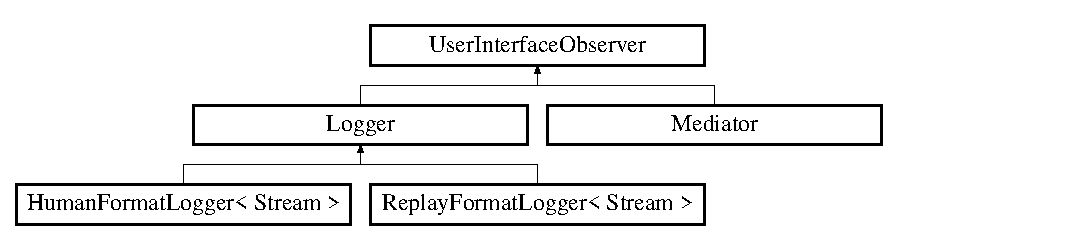
\includegraphics[height=2.78607cm]{classUserInterfaceObserver}
\end{center}
\end{figure}
\subsection*{Public Member Functions}
\begin{DoxyCompactItemize}
\item 
\hypertarget{classUserInterfaceObserver_a99599901a3ae957ef5ae487105d35318}{
virtual void {\bfseries update} (UserInterfaceUpdateContext context, const void $\ast$data)=0}
\label{classUserInterfaceObserver_a99599901a3ae957ef5ae487105d35318}

\end{DoxyCompactItemize}


The documentation for this class was generated from the following files:\begin{DoxyCompactItemize}
\item 
/home/kevin/workspace/HugMe/HugMe v0.9.1/UserInterface/UserInterfaceObserver.h\item 
/home/kevin/workspace/HugMe/HugMe v0.9.1/UserInterface/UserInterfaceObserver.cpp\end{DoxyCompactItemize}

\hypertarget{classUserInterfaceReplayer}{
\section{UserInterfaceReplayer Class Reference}
\label{classUserInterfaceReplayer}\index{UserInterfaceReplayer@{UserInterfaceReplayer}}
}
Inheritance diagram for UserInterfaceReplayer:\begin{figure}[H]
\begin{center}
\leavevmode
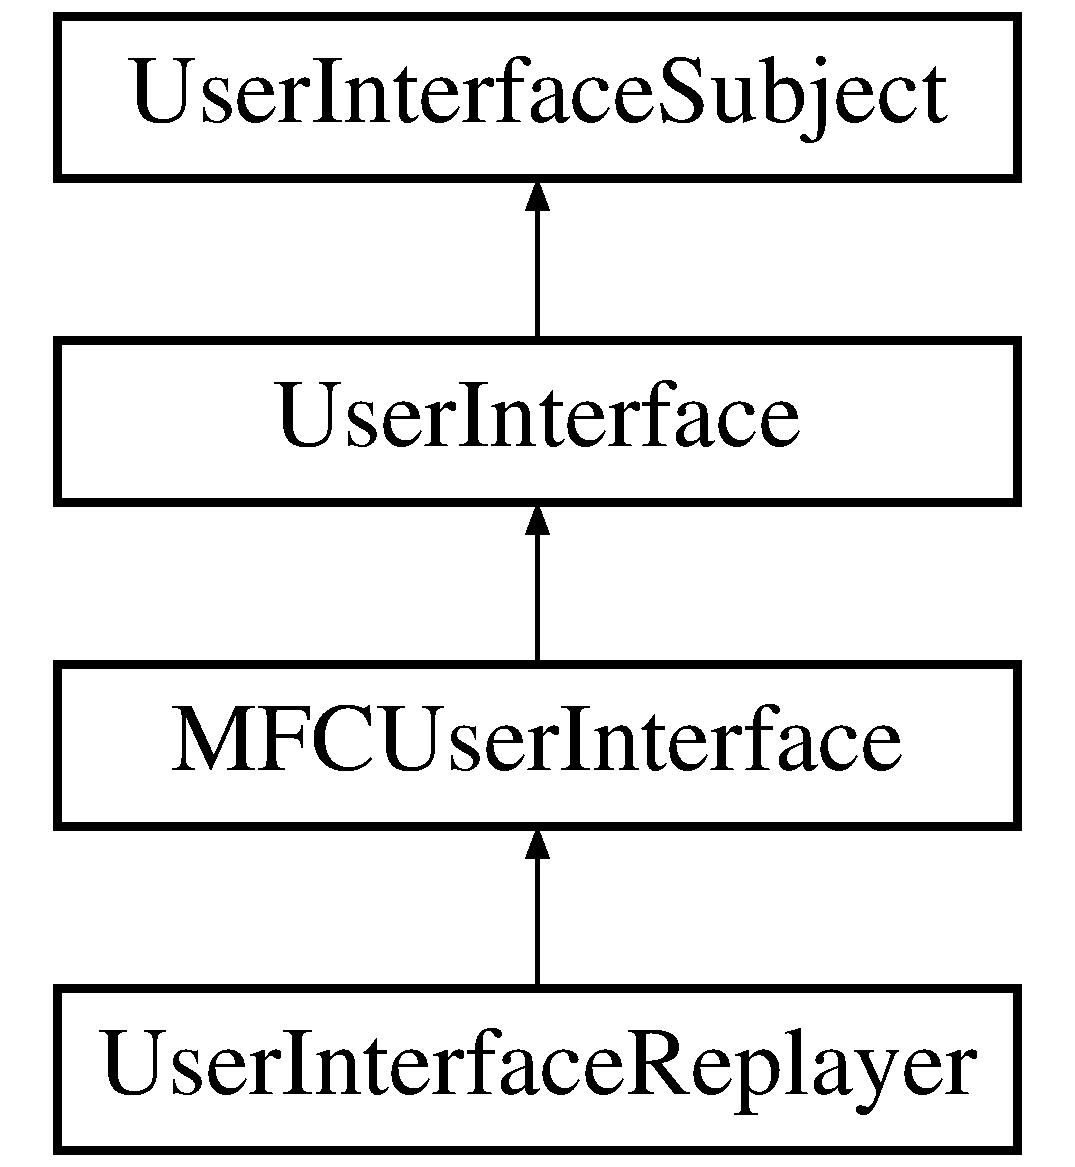
\includegraphics[height=4cm]{classUserInterfaceReplayer}
\end{center}
\end{figure}
\subsection*{Public Member Functions}
\begin{DoxyCompactItemize}
\item 
\hypertarget{classUserInterfaceReplayer_a93c940785e83aaa7860159b39470c49c}{
{\bfseries UserInterfaceReplayer} (const \hyperlink{structUserPreferences}{UserPreferences} \&preferences, boost::shared\_\-ptr$<$ std::ifstream $>$ file, boost::shared\_\-ptr$<$ boost::archive::text\_\-iarchive $>$ archive)}
\label{classUserInterfaceReplayer_a93c940785e83aaa7860159b39470c49c}

\item 
\hypertarget{classUserInterfaceReplayer_a1950dc954873eb5ca01f25a054b63395}{
void {\bfseries replay} (LogEvent\_\-t logEvent)}
\label{classUserInterfaceReplayer_a1950dc954873eb5ca01f25a054b63395}

\end{DoxyCompactItemize}


The documentation for this class was generated from the following files:\begin{DoxyCompactItemize}
\item 
/home/kevin/workspace/HugMe/HugMe v0.9.1/Replay/UserInterfaceReplayer.h\item 
/home/kevin/workspace/HugMe/HugMe v0.9.1/Replay/UserInterfaceReplayer.cpp\end{DoxyCompactItemize}

\hypertarget{classUserInterfaceSubject}{
\section{UserInterfaceSubject Class Reference}
\label{classUserInterfaceSubject}\index{UserInterfaceSubject@{UserInterfaceSubject}}
}
Inheritance diagram for UserInterfaceSubject:\begin{figure}[H]
\begin{center}
\leavevmode
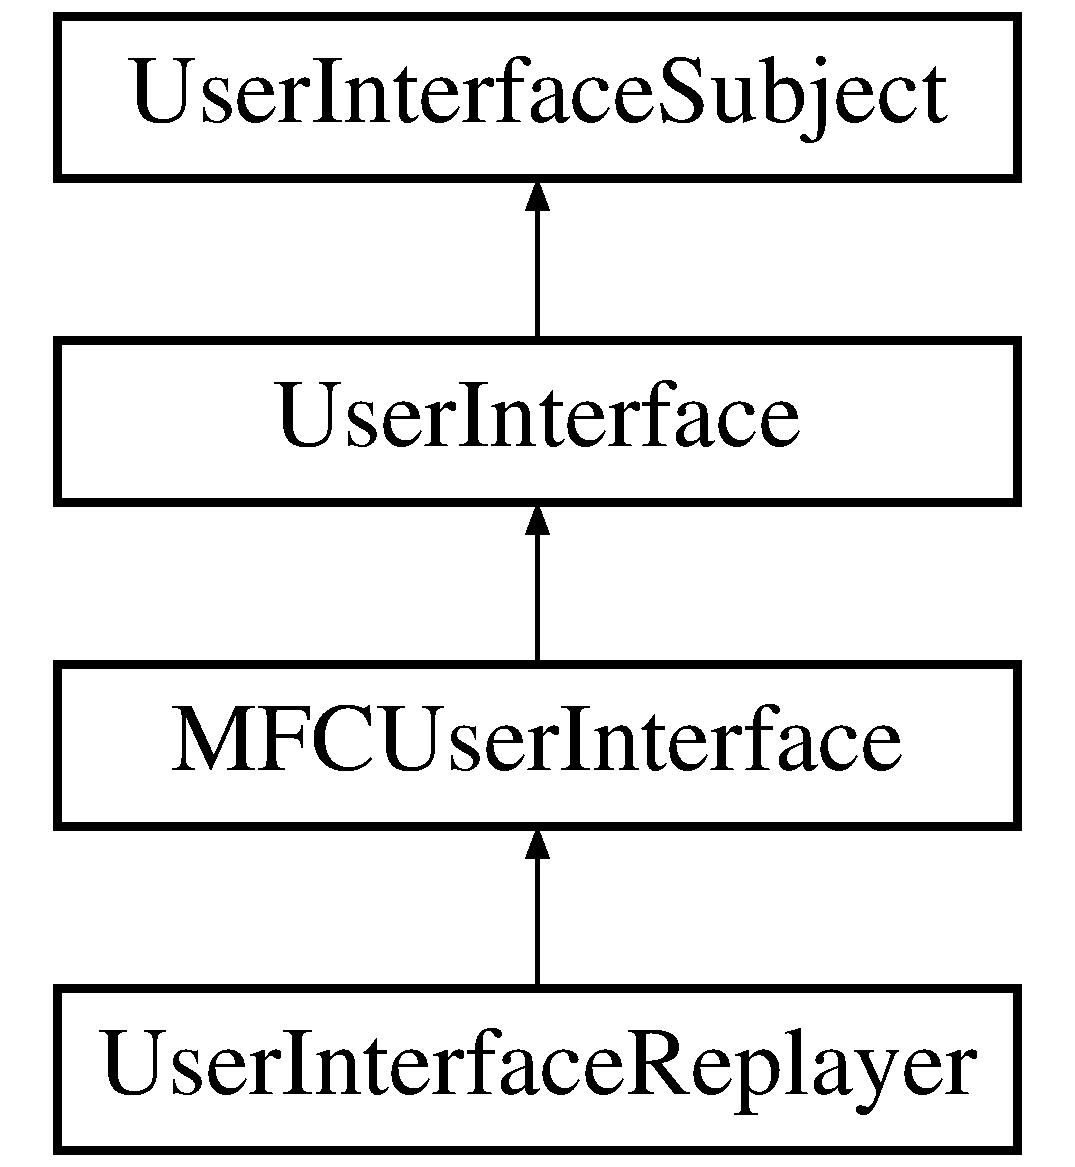
\includegraphics[height=4.000000cm]{classUserInterfaceSubject}
\end{center}
\end{figure}
\subsection*{Public Member Functions}
\begin{DoxyCompactItemize}
\item 
\hypertarget{classUserInterfaceSubject_ac7883808bd4089614b378a8a5309b9c5}{
void {\bfseries attach} (\hyperlink{classUserInterfaceObserver}{UserInterfaceObserver} $\ast$observer)}
\label{classUserInterfaceSubject_ac7883808bd4089614b378a8a5309b9c5}

\item 
\hypertarget{classUserInterfaceSubject_a6b897c262b4f349da028dd91a8683d7e}{
void {\bfseries detach} (\hyperlink{classUserInterfaceObserver}{UserInterfaceObserver} $\ast$observer)}
\label{classUserInterfaceSubject_a6b897c262b4f349da028dd91a8683d7e}

\item 
\hypertarget{classUserInterfaceSubject_a42cbee9b83c54ca6c92d66b0385b2925}{
void {\bfseries notify} (UserInterfaceUpdateContext context, const void $\ast$data=NULL)}
\label{classUserInterfaceSubject_a42cbee9b83c54ca6c92d66b0385b2925}

\end{DoxyCompactItemize}


The documentation for this class was generated from the following files:\begin{DoxyCompactItemize}
\item 
/home/kevin/workspace/HugMe/HugMe v0.9.1/UserInterface/UserInterfaceSubject.h\item 
/home/kevin/workspace/HugMe/HugMe v0.9.1/UserInterface/UserInterfaceSubject.cpp\end{DoxyCompactItemize}

\hypertarget{structUserPreferences}{
\section{UserPreferences Struct Reference}
\label{structUserPreferences}\index{UserPreferences@{UserPreferences}}
}


Represents the user preferences.  




{\ttfamily \#include $<$UserPreferences.h$>$}

\subsection*{Data Fields}
\begin{DoxyCompactItemize}
\item 
\hypertarget{structUserPreferences_a2b7225f2ddf069be9e4f23f426409020}{
std::string \hyperlink{structUserPreferences_a2b7225f2ddf069be9e4f23f426409020}{ipAddress}}
\label{structUserPreferences_a2b7225f2ddf069be9e4f23f426409020}

\begin{DoxyCompactList}\small\item\em The default ip address to connect to. \item\end{DoxyCompactList}\item 
\hypertarget{structUserPreferences_a38d4e509e3d15d642d5e9517ddffd77e}{
std::string \hyperlink{structUserPreferences_a38d4e509e3d15d642d5e9517ddffd77e}{name}}
\label{structUserPreferences_a38d4e509e3d15d642d5e9517ddffd77e}

\begin{DoxyCompactList}\small\item\em The user name. \item\end{DoxyCompactList}\item 
\hypertarget{structUserPreferences_ac8d206952bf8799e05dbd99ec4bc4a33}{
unsigned int \hyperlink{structUserPreferences_ac8d206952bf8799e05dbd99ec4bc4a33}{armBandPort}}
\label{structUserPreferences_ac8d206952bf8799e05dbd99ec4bc4a33}

\begin{DoxyCompactList}\small\item\em The bluetooth port for the arm band. \item\end{DoxyCompactList}\item 
\hypertarget{structUserPreferences_ad4bc7a7d5215b907953d7a0877dd2dec}{
unsigned int \hyperlink{structUserPreferences_ad4bc7a7d5215b907953d7a0877dd2dec}{jacketPort}}
\label{structUserPreferences_ad4bc7a7d5215b907953d7a0877dd2dec}

\begin{DoxyCompactList}\small\item\em The bluetooth port for the jacket. \item\end{DoxyCompactList}\end{DoxyCompactItemize}
\subsection*{Friends}
\begin{DoxyCompactItemize}
\item 
\hypertarget{structUserPreferences_ac98d07dd8f7b70e16ccb9a01abf56b9c}{
class {\bfseries boost::serialization::access}}
\label{structUserPreferences_ac98d07dd8f7b70e16ccb9a01abf56b9c}

\end{DoxyCompactItemize}


\subsection{Detailed Description}
Represents the user preferences. The user preferencese consist of the following: An ip address which is the default ip to connect to. The user name. The blue tooth port for the arm band. The blue tooth port fot the jacket. 

The documentation for this struct was generated from the following file:\begin{DoxyCompactItemize}
\item 
/home/kevin/workspace/HugMe/HugMe v0.9.1/Common/UserPreferences.h\end{DoxyCompactItemize}

\hypertarget{structVideoData}{
\section{VideoData Struct Reference}
\label{structVideoData}\index{VideoData@{VideoData}}
}
\subsection*{Data Fields}
\begin{DoxyCompactItemize}
\item 
\hypertarget{structVideoData_a5f6935b6a9d244c18ce5e3165e2fe6b4}{
std::vector$<$ BYTE $>$ {\bfseries rgb}}
\label{structVideoData_a5f6935b6a9d244c18ce5e3165e2fe6b4}

\end{DoxyCompactItemize}
\subsection*{Friends}
\begin{DoxyCompactItemize}
\item 
\hypertarget{structVideoData_ac98d07dd8f7b70e16ccb9a01abf56b9c}{
class {\bfseries boost::serialization::access}}
\label{structVideoData_ac98d07dd8f7b70e16ccb9a01abf56b9c}

\end{DoxyCompactItemize}


The documentation for this struct was generated from the following file:\begin{DoxyCompactItemize}
\item 
/home/kevin/workspace/HugMe/HugMe v0.9.1/Common/VideoData.h\end{DoxyCompactItemize}

\hypertarget{classVirtualAvatar}{
\section{VirtualAvatar Class Reference}
\label{classVirtualAvatar}\index{VirtualAvatar@{VirtualAvatar}}
}


Represents an avatar in the 3d environment.  




{\ttfamily \#include $<$VirtualAvatar.h$>$}

\subsection*{Public Member Functions}
\begin{DoxyCompactItemize}
\item 
\hyperlink{classVirtualAvatar_af35317b6992d361235debb2b05d0ecb9}{VirtualAvatar} (cWorld $\ast$world, cVector3d startingPosition, bool isLocal)
\begin{DoxyCompactList}\small\item\em Contructor. \item\end{DoxyCompactList}\item 
\hypertarget{classVirtualAvatar_a804f465f57b7baf6f10cd92b1ed9a907}{
\hyperlink{classVirtualAvatar_a804f465f57b7baf6f10cd92b1ed9a907}{$\sim$VirtualAvatar} (void)}
\label{classVirtualAvatar_a804f465f57b7baf6f10cd92b1ed9a907}

\begin{DoxyCompactList}\small\item\em Destructor. \item\end{DoxyCompactList}\item 
void \hyperlink{classVirtualAvatar_a7055e90972db0a5e8ad47a2e11a04870}{rotate} (double ang)
\begin{DoxyCompactList}\small\item\em Rotate the avatar. \item\end{DoxyCompactList}\item 
void \hyperlink{classVirtualAvatar_a784e340db30cc9cb6cecb47cedd03c1c}{translate} (double ang)
\begin{DoxyCompactList}\small\item\em Translate (move) the avatar. \item\end{DoxyCompactList}\item 
void \hyperlink{classVirtualAvatar_a8f96410a9875f2f4823a1f5f0d0146f3}{updateBoundaries} (double ang, cVector3d position)
\begin{DoxyCompactList}\small\item\em Update boundaries when the avatar is moved or rotated. \item\end{DoxyCompactList}\item 
\hypertarget{classVirtualAvatar_a76eb4880060cb9af5ac602197186d999}{
bool \hyperlink{classVirtualAvatar_a76eb4880060cb9af5ac602197186d999}{isInHitBox} (cVector3d ballPos)}
\label{classVirtualAvatar_a76eb4880060cb9af5ac602197186d999}

\begin{DoxyCompactList}\small\item\em Returns true if the point is in the balls hit box. \item\end{DoxyCompactList}\end{DoxyCompactItemize}


\subsection{Detailed Description}
Represents an avatar in the 3d environment. 

\subsection{Constructor \& Destructor Documentation}
\hypertarget{classVirtualAvatar_af35317b6992d361235debb2b05d0ecb9}{
\index{VirtualAvatar@{VirtualAvatar}!VirtualAvatar@{VirtualAvatar}}
\index{VirtualAvatar@{VirtualAvatar}!VirtualAvatar@{VirtualAvatar}}
\subsubsection[{VirtualAvatar}]{\setlength{\rightskip}{0pt plus 5cm}VirtualAvatar::VirtualAvatar (
\begin{DoxyParamCaption}
\item[{cWorld $\ast$}]{ world, }
\item[{cVector3d}]{ startingPosition, }
\item[{bool}]{ isLocal}
\end{DoxyParamCaption}
)}}
\label{classVirtualAvatar_af35317b6992d361235debb2b05d0ecb9}


Contructor. 


\begin{DoxyParams}{Parameters}
\item[{\em world}]The chai3d world to which the avatar belongs. \item[{\em startingPosition}]The avatar's position. \item[{\em true}]if the avatar is the local avatar. \end{DoxyParams}


\subsection{Member Function Documentation}
\hypertarget{classVirtualAvatar_a7055e90972db0a5e8ad47a2e11a04870}{
\index{VirtualAvatar@{VirtualAvatar}!rotate@{rotate}}
\index{rotate@{rotate}!VirtualAvatar@{VirtualAvatar}}
\subsubsection[{rotate}]{\setlength{\rightskip}{0pt plus 5cm}void VirtualAvatar::rotate (
\begin{DoxyParamCaption}
\item[{double}]{ ang}
\end{DoxyParamCaption}
)}}
\label{classVirtualAvatar_a7055e90972db0a5e8ad47a2e11a04870}


Rotate the avatar. 


\begin{DoxyParams}{Parameters}
\item[{\em ang}]The angle to rotate the avatar to. This angle is absolute to the starting position, not relative. \end{DoxyParams}
\hypertarget{classVirtualAvatar_a784e340db30cc9cb6cecb47cedd03c1c}{
\index{VirtualAvatar@{VirtualAvatar}!translate@{translate}}
\index{translate@{translate}!VirtualAvatar@{VirtualAvatar}}
\subsubsection[{translate}]{\setlength{\rightskip}{0pt plus 5cm}void VirtualAvatar::translate (
\begin{DoxyParamCaption}
\item[{double}]{ ang}
\end{DoxyParamCaption}
)}}
\label{classVirtualAvatar_a784e340db30cc9cb6cecb47cedd03c1c}


Translate (move) the avatar. 


\begin{DoxyParams}{Parameters}
\item[{\em ang}]The angle to which the avatar was rotated. \end{DoxyParams}
\hypertarget{classVirtualAvatar_a8f96410a9875f2f4823a1f5f0d0146f3}{
\index{VirtualAvatar@{VirtualAvatar}!updateBoundaries@{updateBoundaries}}
\index{updateBoundaries@{updateBoundaries}!VirtualAvatar@{VirtualAvatar}}
\subsubsection[{updateBoundaries}]{\setlength{\rightskip}{0pt plus 5cm}void VirtualAvatar::updateBoundaries (
\begin{DoxyParamCaption}
\item[{double}]{ ang, }
\item[{cVector3d}]{ position}
\end{DoxyParamCaption}
)}}
\label{classVirtualAvatar_a8f96410a9875f2f4823a1f5f0d0146f3}


Update boundaries when the avatar is moved or rotated. 


\begin{DoxyParams}{Parameters}
\item[{\em ang}]The angle from which the avatar was moved. \item[{\em position}]The avatar's position. \end{DoxyParams}


The documentation for this class was generated from the following files:\begin{DoxyCompactItemize}
\item 
/home/kevin/workspace/HugMe/HugMe v0.9.1/Game/VirtualAvatar.h\item 
/home/kevin/workspace/HugMe/HugMe v0.9.1/Game/VirtualAvatar.cpp\end{DoxyCompactItemize}

\hypertarget{classVirtualBall}{
\section{VirtualBall Class Reference}
\label{classVirtualBall}\index{VirtualBall@{VirtualBall}}
}


Represents a ball in the 3d environment.  




{\ttfamily \#include $<$VirtualBall.h$>$}

\subsection*{Public Member Functions}
\begin{DoxyCompactItemize}
\item 
\hyperlink{classVirtualBall_ac23e87ff7e9311a6eec9534cf7c4ad19}{VirtualBall} (cWorld $\ast$world, cODEWorld $\ast$ODEWorld)
\begin{DoxyCompactList}\small\item\em Constructor. \item\end{DoxyCompactList}\item 
\hypertarget{classVirtualBall_af8e24103797c63c53886dc82fcab09e8}{
\hyperlink{classVirtualBall_af8e24103797c63c53886dc82fcab09e8}{$\sim$VirtualBall} ()}
\label{classVirtualBall_af8e24103797c63c53886dc82fcab09e8}

\begin{DoxyCompactList}\small\item\em Destructor. \item\end{DoxyCompactList}\item 
void \hyperlink{classVirtualBall_a886d85950bb75ca63c2583e1a0ac9211}{fire} (\hyperlink{classProjectile}{Projectile} p)
\begin{DoxyCompactList}\small\item\em Fire the ball. \item\end{DoxyCompactList}\item 
cVector3d \hyperlink{classVirtualBall_a4477ee504d911d89d66dd1c61aa0fcb1}{getMeshPos} ()
\begin{DoxyCompactList}\small\item\em Get the ball's position. \item\end{DoxyCompactList}\end{DoxyCompactItemize}


\subsection{Detailed Description}
Represents a ball in the 3d environment. 

\subsection{Constructor \& Destructor Documentation}
\hypertarget{classVirtualBall_ac23e87ff7e9311a6eec9534cf7c4ad19}{
\index{VirtualBall@{VirtualBall}!VirtualBall@{VirtualBall}}
\index{VirtualBall@{VirtualBall}!VirtualBall@{VirtualBall}}
\subsubsection[{VirtualBall}]{\setlength{\rightskip}{0pt plus 5cm}VirtualBall::VirtualBall (
\begin{DoxyParamCaption}
\item[{cWorld $\ast$}]{ world, }
\item[{cODEWorld $\ast$}]{ ODEWorld}
\end{DoxyParamCaption}
)}}
\label{classVirtualBall_ac23e87ff7e9311a6eec9534cf7c4ad19}


Constructor. 


\begin{DoxyParams}{Parameters}
\item[{\em world}]The chai3d world to which the ball belongs. \item[{\em ODEWorld}]The physical world to which the ball belongs. \end{DoxyParams}


\subsection{Member Function Documentation}
\hypertarget{classVirtualBall_a886d85950bb75ca63c2583e1a0ac9211}{
\index{VirtualBall@{VirtualBall}!fire@{fire}}
\index{fire@{fire}!VirtualBall@{VirtualBall}}
\subsubsection[{fire}]{\setlength{\rightskip}{0pt plus 5cm}void VirtualBall::fire (
\begin{DoxyParamCaption}
\item[{{\bf Projectile}}]{ p}
\end{DoxyParamCaption}
)}}
\label{classVirtualBall_a886d85950bb75ca63c2583e1a0ac9211}


Fire the ball. 

The ball will take the position of the passed projectile and it will be applied the force of the passed projectile. 
\begin{DoxyParams}{Parameters}
\item[{\em p}]The projectile which the ball will become. \end{DoxyParams}
\hypertarget{classVirtualBall_a4477ee504d911d89d66dd1c61aa0fcb1}{
\index{VirtualBall@{VirtualBall}!getMeshPos@{getMeshPos}}
\index{getMeshPos@{getMeshPos}!VirtualBall@{VirtualBall}}
\subsubsection[{getMeshPos}]{\setlength{\rightskip}{0pt plus 5cm}cVector3d VirtualBall::getMeshPos (
\begin{DoxyParamCaption}
{}
\end{DoxyParamCaption}
)}}
\label{classVirtualBall_a4477ee504d911d89d66dd1c61aa0fcb1}


Get the ball's position. 

\begin{DoxyReturn}{Returns}
The position of the ball. 
\end{DoxyReturn}


The documentation for this class was generated from the following files:\begin{DoxyCompactItemize}
\item 
/home/kevin/workspace/HugMe/HugMe v0.9.1/Game/VirtualBall.h\item 
/home/kevin/workspace/HugMe/HugMe v0.9.1/Game/VirtualBall.cpp\end{DoxyCompactItemize}

\hypertarget{classVirtualEnvironment}{
\section{VirtualEnvironment Class Reference}
\label{classVirtualEnvironment}\index{VirtualEnvironment@{VirtualEnvironment}}
}


The virtual environment is the 3d environment in which the game is played.  




{\ttfamily \#include $<$VirtualEnvironment.h$>$}

\subsection*{Public Member Functions}
\begin{DoxyCompactItemize}
\item 
\hypertarget{classVirtualEnvironment_ae0e38db3924687d121dfbda86e1d9b72}{
\hyperlink{classVirtualEnvironment_ae0e38db3924687d121dfbda86e1d9b72}{VirtualEnvironment} (void)}
\label{classVirtualEnvironment_ae0e38db3924687d121dfbda86e1d9b72}

\begin{DoxyCompactList}\small\item\em Constructor. \item\end{DoxyCompactList}\item 
\hypertarget{classVirtualEnvironment_a5e8b1b63923dd31b8574f88f18007da5}{
\hyperlink{classVirtualEnvironment_a5e8b1b63923dd31b8574f88f18007da5}{$\sim$VirtualEnvironment} (void)}
\label{classVirtualEnvironment_a5e8b1b63923dd31b8574f88f18007da5}

\begin{DoxyCompactList}\small\item\em Destructor. \item\end{DoxyCompactList}\item 
cCamera $\ast$ \hyperlink{classVirtualEnvironment_afd987f6e88168c734aee6689efb64e5b}{camera} ()
\begin{DoxyCompactList}\small\item\em Get the environments camera. \item\end{DoxyCompactList}\item 
void \hyperlink{classVirtualEnvironment_ab34e50a795e4b872f24b2d604a5464f7}{moveLocalSlingshot} (cVector3d position)
\begin{DoxyCompactList}\small\item\em Move the local slingshot to a new position. \item\end{DoxyCompactList}\item 
void \hyperlink{classVirtualEnvironment_a24bc3eec1917751a16f4ac510f06affc}{movePeerSlingshot} (cVector3d position)
\begin{DoxyCompactList}\small\item\em Move the peer slingshot to a new position. \item\end{DoxyCompactList}\item 
void \hyperlink{classVirtualEnvironment_a73345d04770c2080b1e102fb9457c3d3}{moveLocalAvatar} (cVector3d position)
\begin{DoxyCompactList}\small\item\em Move the local avatar to a new position. \item\end{DoxyCompactList}\item 
void \hyperlink{classVirtualEnvironment_ab0dea50eb3ff01720a539ec669d07e54}{movePeerAvatar} (cVector3d position)
\begin{DoxyCompactList}\small\item\em Move the peer avatar to a new position. \item\end{DoxyCompactList}\item 
void \hyperlink{classVirtualEnvironment_a8cd7268b0e8339cad855715a9a7b6c7f}{reduceLocalHp} (int dmg)
\begin{DoxyCompactList}\small\item\em Reduce the hit points on the local player. \item\end{DoxyCompactList}\item 
void \hyperlink{classVirtualEnvironment_a6e2c1d962098ed2b16b11aac8fe79380}{reducePeerHp} (int dmg)
\begin{DoxyCompactList}\small\item\em Reduce the hit points on the peer player. \item\end{DoxyCompactList}\item 
\hyperlink{classProjectile}{Projectile} \hyperlink{classVirtualEnvironment_a05831f68bb623ab852a52180b92b6efb}{fireLocalSlingshot} ()
\begin{DoxyCompactList}\small\item\em Shoot a projectile from the local slingshot. \item\end{DoxyCompactList}\item 
void \hyperlink{classVirtualEnvironment_a3eb4771f3cd9cba993c9cdc0b8d0271f}{firePeerSlingshot} (\hyperlink{classProjectile}{Projectile} p)
\begin{DoxyCompactList}\small\item\em Shoot a projectile from the peer's slingshot. \item\end{DoxyCompactList}\item 
void \hyperlink{classVirtualEnvironment_a8490579021c2abeef1dba404bab86db9}{initialize} (void)
\begin{DoxyCompactList}\small\item\em Initialize the 3d environment. \item\end{DoxyCompactList}\item 
void \hyperlink{classVirtualEnvironment_adff43d5572e61995b167ea0bc532d1c4}{updateFrame} ()
\begin{DoxyCompactList}\small\item\em Update the frame. \item\end{DoxyCompactList}\item 
bool \hyperlink{classVirtualEnvironment_aacb8b90cc65753c95c2c4a6a9bc9f51b}{isColliding} ()
\begin{DoxyCompactList}\small\item\em Check if an object is colliding with the local player. \item\end{DoxyCompactList}\end{DoxyCompactItemize}


\subsection{Detailed Description}
The virtual environment is the 3d environment in which the game is played. This class contains all the 3d objects that make up our game. The environment is implemented using the chai3d library. This class is responsible for all modifications to the environment. 

\subsection{Member Function Documentation}
\hypertarget{classVirtualEnvironment_afd987f6e88168c734aee6689efb64e5b}{
\index{VirtualEnvironment@{VirtualEnvironment}!camera@{camera}}
\index{camera@{camera}!VirtualEnvironment@{VirtualEnvironment}}
\subsubsection[{camera}]{\setlength{\rightskip}{0pt plus 5cm}cCamera $\ast$ VirtualEnvironment::camera (
\begin{DoxyParamCaption}
{}
\end{DoxyParamCaption}
)}}
\label{classVirtualEnvironment_afd987f6e88168c734aee6689efb64e5b}


Get the environments camera. 

\begin{DoxyReturn}{Returns}
the camera 
\end{DoxyReturn}
\hypertarget{classVirtualEnvironment_a05831f68bb623ab852a52180b92b6efb}{
\index{VirtualEnvironment@{VirtualEnvironment}!fireLocalSlingshot@{fireLocalSlingshot}}
\index{fireLocalSlingshot@{fireLocalSlingshot}!VirtualEnvironment@{VirtualEnvironment}}
\subsubsection[{fireLocalSlingshot}]{\setlength{\rightskip}{0pt plus 5cm}{\bf Projectile} VirtualEnvironment::fireLocalSlingshot (
\begin{DoxyParamCaption}
{}
\end{DoxyParamCaption}
)}}
\label{classVirtualEnvironment_a05831f68bb623ab852a52180b92b6efb}


Shoot a projectile from the local slingshot. 

\begin{DoxyReturn}{Returns}
The projectile that was just fired 
\end{DoxyReturn}
\hypertarget{classVirtualEnvironment_a3eb4771f3cd9cba993c9cdc0b8d0271f}{
\index{VirtualEnvironment@{VirtualEnvironment}!firePeerSlingshot@{firePeerSlingshot}}
\index{firePeerSlingshot@{firePeerSlingshot}!VirtualEnvironment@{VirtualEnvironment}}
\subsubsection[{firePeerSlingshot}]{\setlength{\rightskip}{0pt plus 5cm}void VirtualEnvironment::firePeerSlingshot (
\begin{DoxyParamCaption}
\item[{{\bf Projectile}}]{ p}
\end{DoxyParamCaption}
)}}
\label{classVirtualEnvironment_a3eb4771f3cd9cba993c9cdc0b8d0271f}


Shoot a projectile from the peer's slingshot. 


\begin{DoxyParams}{Parameters}
\item[{\em p}]The projectile to be fired \end{DoxyParams}
\hypertarget{classVirtualEnvironment_a8490579021c2abeef1dba404bab86db9}{
\index{VirtualEnvironment@{VirtualEnvironment}!initialize@{initialize}}
\index{initialize@{initialize}!VirtualEnvironment@{VirtualEnvironment}}
\subsubsection[{initialize}]{\setlength{\rightskip}{0pt plus 5cm}void VirtualEnvironment::initialize (
\begin{DoxyParamCaption}
\item[{void}]{}
\end{DoxyParamCaption}
)}}
\label{classVirtualEnvironment_a8490579021c2abeef1dba404bab86db9}


Initialize the 3d environment. 

This initializes all the 3d objects. \hypertarget{classVirtualEnvironment_aacb8b90cc65753c95c2c4a6a9bc9f51b}{
\index{VirtualEnvironment@{VirtualEnvironment}!isColliding@{isColliding}}
\index{isColliding@{isColliding}!VirtualEnvironment@{VirtualEnvironment}}
\subsubsection[{isColliding}]{\setlength{\rightskip}{0pt plus 5cm}bool VirtualEnvironment::isColliding (
\begin{DoxyParamCaption}
{}
\end{DoxyParamCaption}
)}}
\label{classVirtualEnvironment_aacb8b90cc65753c95c2c4a6a9bc9f51b}


Check if an object is colliding with the local player. 

\begin{DoxyReturn}{Returns}
true If an object is hitting the local player. 
\end{DoxyReturn}
\hypertarget{classVirtualEnvironment_a73345d04770c2080b1e102fb9457c3d3}{
\index{VirtualEnvironment@{VirtualEnvironment}!moveLocalAvatar@{moveLocalAvatar}}
\index{moveLocalAvatar@{moveLocalAvatar}!VirtualEnvironment@{VirtualEnvironment}}
\subsubsection[{moveLocalAvatar}]{\setlength{\rightskip}{0pt plus 5cm}void VirtualEnvironment::moveLocalAvatar (
\begin{DoxyParamCaption}
\item[{cVector3d}]{ position}
\end{DoxyParamCaption}
)}}
\label{classVirtualEnvironment_a73345d04770c2080b1e102fb9457c3d3}


Move the local avatar to a new position. 


\begin{DoxyParams}{Parameters}
\item[{\em position}]The new position \end{DoxyParams}
\hypertarget{classVirtualEnvironment_ab34e50a795e4b872f24b2d604a5464f7}{
\index{VirtualEnvironment@{VirtualEnvironment}!moveLocalSlingshot@{moveLocalSlingshot}}
\index{moveLocalSlingshot@{moveLocalSlingshot}!VirtualEnvironment@{VirtualEnvironment}}
\subsubsection[{moveLocalSlingshot}]{\setlength{\rightskip}{0pt plus 5cm}void VirtualEnvironment::moveLocalSlingshot (
\begin{DoxyParamCaption}
\item[{cVector3d}]{ position}
\end{DoxyParamCaption}
)}}
\label{classVirtualEnvironment_ab34e50a795e4b872f24b2d604a5464f7}


Move the local slingshot to a new position. 


\begin{DoxyParams}{Parameters}
\item[{\em position}]The new position \end{DoxyParams}
\hypertarget{classVirtualEnvironment_ab0dea50eb3ff01720a539ec669d07e54}{
\index{VirtualEnvironment@{VirtualEnvironment}!movePeerAvatar@{movePeerAvatar}}
\index{movePeerAvatar@{movePeerAvatar}!VirtualEnvironment@{VirtualEnvironment}}
\subsubsection[{movePeerAvatar}]{\setlength{\rightskip}{0pt plus 5cm}void VirtualEnvironment::movePeerAvatar (
\begin{DoxyParamCaption}
\item[{cVector3d}]{ position}
\end{DoxyParamCaption}
)}}
\label{classVirtualEnvironment_ab0dea50eb3ff01720a539ec669d07e54}


Move the peer avatar to a new position. 


\begin{DoxyParams}{Parameters}
\item[{\em position}]The new position \end{DoxyParams}
\hypertarget{classVirtualEnvironment_a24bc3eec1917751a16f4ac510f06affc}{
\index{VirtualEnvironment@{VirtualEnvironment}!movePeerSlingshot@{movePeerSlingshot}}
\index{movePeerSlingshot@{movePeerSlingshot}!VirtualEnvironment@{VirtualEnvironment}}
\subsubsection[{movePeerSlingshot}]{\setlength{\rightskip}{0pt plus 5cm}void VirtualEnvironment::movePeerSlingshot (
\begin{DoxyParamCaption}
\item[{cVector3d}]{ position}
\end{DoxyParamCaption}
)}}
\label{classVirtualEnvironment_a24bc3eec1917751a16f4ac510f06affc}


Move the peer slingshot to a new position. 


\begin{DoxyParams}{Parameters}
\item[{\em position}]The new position \end{DoxyParams}
\hypertarget{classVirtualEnvironment_a8cd7268b0e8339cad855715a9a7b6c7f}{
\index{VirtualEnvironment@{VirtualEnvironment}!reduceLocalHp@{reduceLocalHp}}
\index{reduceLocalHp@{reduceLocalHp}!VirtualEnvironment@{VirtualEnvironment}}
\subsubsection[{reduceLocalHp}]{\setlength{\rightskip}{0pt plus 5cm}void VirtualEnvironment::reduceLocalHp (
\begin{DoxyParamCaption}
\item[{int}]{ dmg}
\end{DoxyParamCaption}
)}}
\label{classVirtualEnvironment_a8cd7268b0e8339cad855715a9a7b6c7f}


Reduce the hit points on the local player. 


\begin{DoxyParams}{Parameters}
\item[{\em dmg}]The amount of hit points to remove. \end{DoxyParams}
\hypertarget{classVirtualEnvironment_a6e2c1d962098ed2b16b11aac8fe79380}{
\index{VirtualEnvironment@{VirtualEnvironment}!reducePeerHp@{reducePeerHp}}
\index{reducePeerHp@{reducePeerHp}!VirtualEnvironment@{VirtualEnvironment}}
\subsubsection[{reducePeerHp}]{\setlength{\rightskip}{0pt plus 5cm}void VirtualEnvironment::reducePeerHp (
\begin{DoxyParamCaption}
\item[{int}]{ dmg}
\end{DoxyParamCaption}
)}}
\label{classVirtualEnvironment_a6e2c1d962098ed2b16b11aac8fe79380}


Reduce the hit points on the peer player. 


\begin{DoxyParams}{Parameters}
\item[{\em dmg}]The amount of hit points to remove. \end{DoxyParams}
\hypertarget{classVirtualEnvironment_adff43d5572e61995b167ea0bc532d1c4}{
\index{VirtualEnvironment@{VirtualEnvironment}!updateFrame@{updateFrame}}
\index{updateFrame@{updateFrame}!VirtualEnvironment@{VirtualEnvironment}}
\subsubsection[{updateFrame}]{\setlength{\rightskip}{0pt plus 5cm}void VirtualEnvironment::updateFrame (
\begin{DoxyParamCaption}
{}
\end{DoxyParamCaption}
)}}
\label{classVirtualEnvironment_adff43d5572e61995b167ea0bc532d1c4}


Update the frame. 

This will update the frame to display the latest changes. This is where the physics are calculated and object positions are updated. 

The documentation for this class was generated from the following files:\begin{DoxyCompactItemize}
\item 
/home/kevin/workspace/HugMe/HugMe v0.9.1/Game/VirtualEnvironment.h\item 
/home/kevin/workspace/HugMe/HugMe v0.9.1/Game/VirtualEnvironment.cpp\end{DoxyCompactItemize}

\hypertarget{classVirtualSlingshot}{
\section{VirtualSlingshot Class Reference}
\label{classVirtualSlingshot}\index{VirtualSlingshot@{VirtualSlingshot}}
}
\subsection*{Public Member Functions}
\begin{DoxyCompactItemize}
\item 
\hypertarget{classVirtualSlingshot_a5103bd90514183171736a73c02bb1940}{
{\bfseries VirtualSlingshot} (cWorld $\ast$world, const cVector3d startingPosition)}
\label{classVirtualSlingshot_a5103bd90514183171736a73c02bb1940}

\item 
\hypertarget{classVirtualSlingshot_ab1b888f0b9982ced892d3f4ad6cc5eb9}{
void {\bfseries move} (cVector3d position)}
\label{classVirtualSlingshot_ab1b888f0b9982ced892d3f4ad6cc5eb9}

\item 
\hypertarget{classVirtualSlingshot_a6ab9b13ce2ed3d9a5c4b7d09e844a62f}{
cVector3d {\bfseries getBallPosition} ()}
\label{classVirtualSlingshot_a6ab9b13ce2ed3d9a5c4b7d09e844a62f}

\end{DoxyCompactItemize}


The documentation for this class was generated from the following files:\begin{DoxyCompactItemize}
\item 
/home/kevin/workspace/HugMe/HugMe v0.9.1/Game/VirtualSlingshot.h\item 
/home/kevin/workspace/HugMe/HugMe v0.9.1/Game/VirtualSlingshot.cpp\end{DoxyCompactItemize}

\hypertarget{classWinsockNetwork}{
\section{WinsockNetwork Class Reference}
\label{classWinsockNetwork}\index{WinsockNetwork@{WinsockNetwork}}
}
Inheritance diagram for WinsockNetwork:\begin{figure}[H]
\begin{center}
\leavevmode
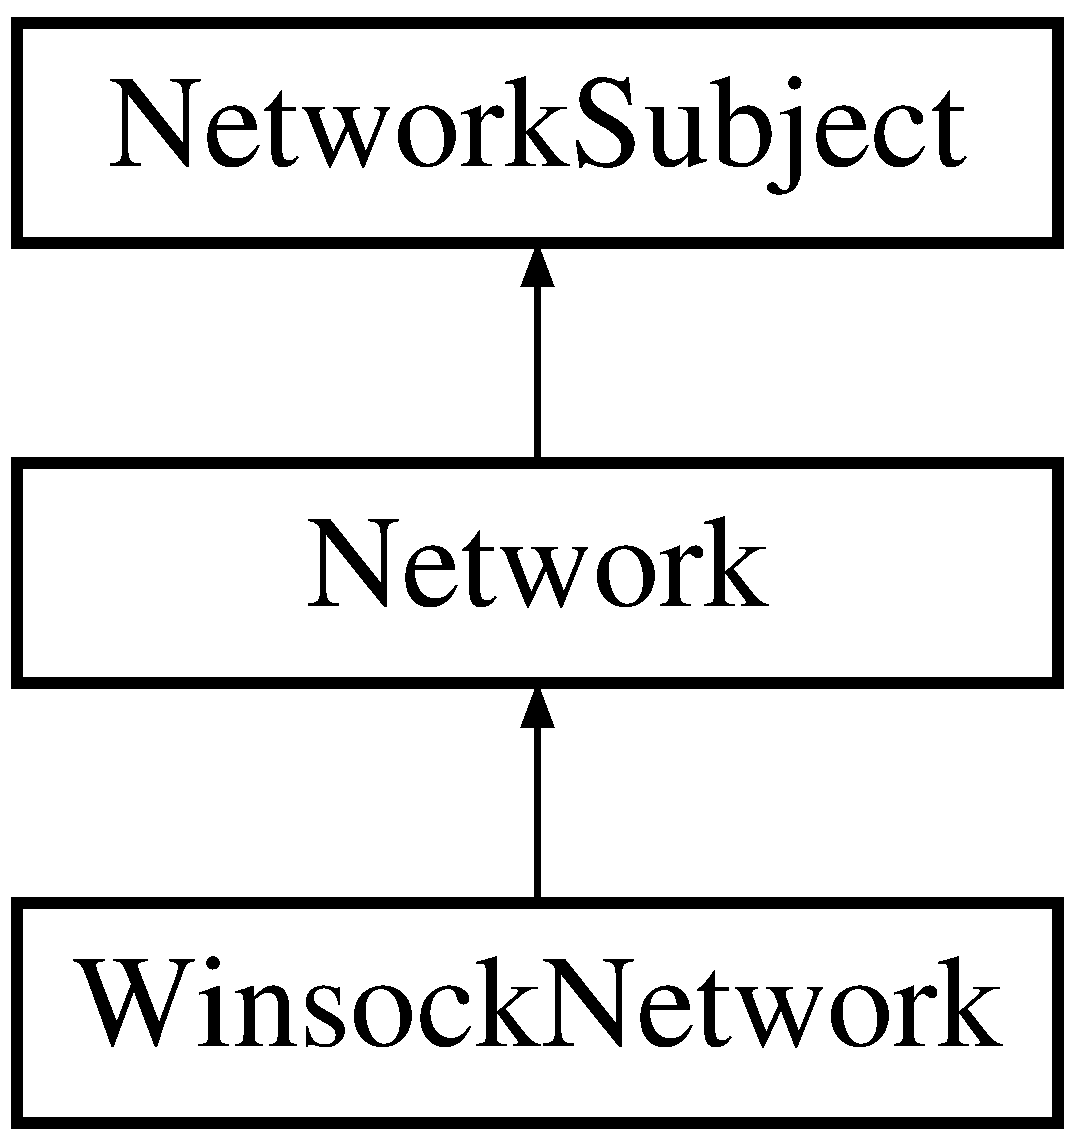
\includegraphics[height=3cm]{classWinsockNetwork}
\end{center}
\end{figure}
\subsection*{Public Member Functions}
\begin{DoxyCompactItemize}
\item 
\hypertarget{classWinsockNetwork_a6f2f806a0e246a46ff6d0c2006cddd43}{
virtual rc\_\-network {\bfseries listen} (const std::string \&userName)}
\label{classWinsockNetwork_a6f2f806a0e246a46ff6d0c2006cddd43}

\item 
\hypertarget{classWinsockNetwork_a0f7f289635183b1082894f230a989006}{
virtual rc\_\-network {\bfseries connect} (const std::string \&ipAddress, const std::string \&userName)}
\label{classWinsockNetwork_a0f7f289635183b1082894f230a989006}

\item 
\hypertarget{classWinsockNetwork_abd947a2edb4d5053286f25b4c9f041c1}{
virtual rc\_\-network {\bfseries disconnect} ()}
\label{classWinsockNetwork_abd947a2edb4d5053286f25b4c9f041c1}

\item 
\hypertarget{classWinsockNetwork_ae76b6c306ef15d162fe652c38c78d4e2}{
virtual rc\_\-network {\bfseries sendUserName} (const std::string \&userName)}
\label{classWinsockNetwork_ae76b6c306ef15d162fe652c38c78d4e2}

\item 
\hypertarget{classWinsockNetwork_a420d4e6b5c698476a94dcdb503233de7}{
virtual rc\_\-network {\bfseries sendChatMessage} (const std::string \&message)}
\label{classWinsockNetwork_a420d4e6b5c698476a94dcdb503233de7}

\item 
\hypertarget{classWinsockNetwork_a20ed4411ec34336c6a213b15cc3fcad9}{
virtual rc\_\-network {\bfseries sendStartGame} ()}
\label{classWinsockNetwork_a20ed4411ec34336c6a213b15cc3fcad9}

\item 
\hypertarget{classWinsockNetwork_ae4412629d2ee052afc41c81f36cfad50}{
virtual rc\_\-network {\bfseries sendPauseGame} ()}
\label{classWinsockNetwork_ae4412629d2ee052afc41c81f36cfad50}

\item 
\hypertarget{classWinsockNetwork_a877c8001bbd880295e0458c3377dca25}{
virtual rc\_\-network {\bfseries sendEndGame} ()}
\label{classWinsockNetwork_a877c8001bbd880295e0458c3377dca25}

\item 
\hypertarget{classWinsockNetwork_a36362dbaa70fbe00dd48fded21464888}{
virtual rc\_\-network {\bfseries sendVideoData} (const \hyperlink{structVideoData}{VideoData} \&video)}
\label{classWinsockNetwork_a36362dbaa70fbe00dd48fded21464888}

\item 
\hypertarget{classWinsockNetwork_ab27dd7393a89573f9e75e1a50efbc833}{
virtual rc\_\-network {\bfseries sendPlayerPosition} (const cVector3d \&position)}
\label{classWinsockNetwork_ab27dd7393a89573f9e75e1a50efbc833}

\item 
\hypertarget{classWinsockNetwork_af0456294cf39244cc59f1ca81e2aa2d3}{
virtual rc\_\-network {\bfseries sendSlingshotPosition} (const cVector3d \&position)}
\label{classWinsockNetwork_af0456294cf39244cc59f1ca81e2aa2d3}

\item 
\hypertarget{classWinsockNetwork_accb610c314dd94a1649bcfe101c93997}{
virtual rc\_\-network {\bfseries sendProjectile} (const \hyperlink{classProjectile}{Projectile} \&projectile)}
\label{classWinsockNetwork_accb610c314dd94a1649bcfe101c93997}

\item 
\hypertarget{classWinsockNetwork_a0a8ced3a30f215e71114b9fa94b3d1e3}{
virtual rc\_\-network {\bfseries sendSlingshotPullback} ()}
\label{classWinsockNetwork_a0a8ced3a30f215e71114b9fa94b3d1e3}

\item 
\hypertarget{classWinsockNetwork_ac4076b605f2378bf8728be6730512f95}{
virtual rc\_\-network {\bfseries sendSlingshotRelease} ()}
\label{classWinsockNetwork_ac4076b605f2378bf8728be6730512f95}

\item 
\hypertarget{classWinsockNetwork_a8c621566b7ce641d86797569346fcaad}{
virtual bool {\bfseries isConnected} () const }
\label{classWinsockNetwork_a8c621566b7ce641d86797569346fcaad}

\item 
\hypertarget{classWinsockNetwork_a7cbc0e15323359b9bdb862342e406f23}{
virtual bool {\bfseries isListening} () const }
\label{classWinsockNetwork_a7cbc0e15323359b9bdb862342e406f23}

\item 
\hypertarget{classWinsockNetwork_a011b39d509309dd98f3b798e7c6b7c62}{
void {\bfseries notifyAccept} (\hyperlink{classNetworkSocket}{NetworkSocket} $\ast$socket)}
\label{classWinsockNetwork_a011b39d509309dd98f3b798e7c6b7c62}

\end{DoxyCompactItemize}


The documentation for this class was generated from the following files:\begin{DoxyCompactItemize}
\item 
/home/kevin/workspace/HugMe/HugMe v0.9.1/Network/WinsockNetwork.h\item 
/home/kevin/workspace/HugMe/HugMe v0.9.1/Network/WinsockNetwork.cpp\end{DoxyCompactItemize}

\hypertarget{classZCamera}{
\section{ZCamera Class Reference}
\label{classZCamera}\index{ZCamera@{ZCamera}}
}
Inheritance diagram for ZCamera:\begin{figure}[H]
\begin{center}
\leavevmode
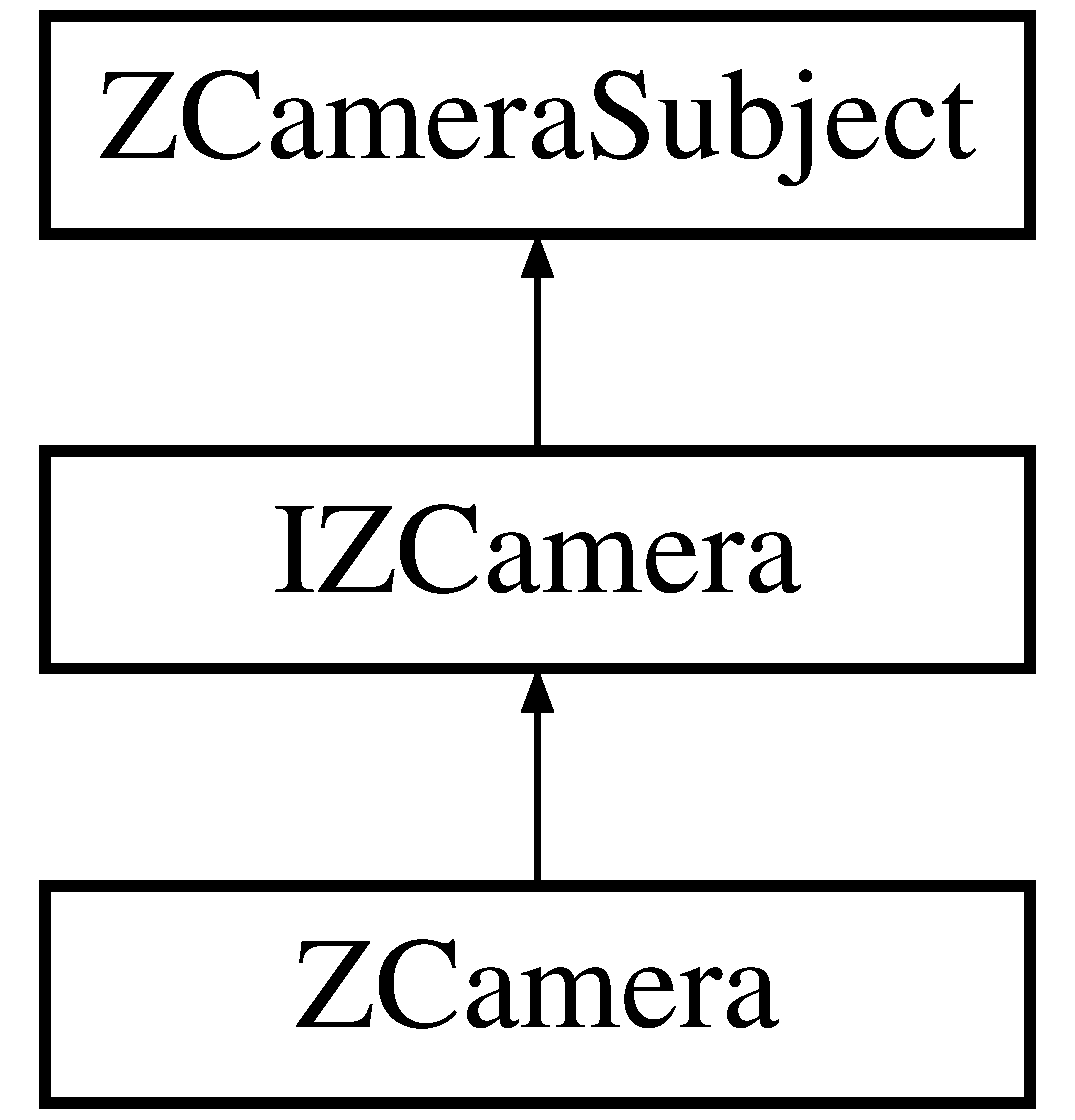
\includegraphics[height=3cm]{classZCamera}
\end{center}
\end{figure}
\subsection*{Public Member Functions}
\begin{DoxyCompactItemize}
\item 
\hypertarget{classZCamera_a9eb62d7424767779dc46cc357ae77645}{
virtual void {\bfseries startCapture} ()}
\label{classZCamera_a9eb62d7424767779dc46cc357ae77645}

\item 
\hypertarget{classZCamera_af883a28008906c04065644c5e8eb4e40}{
virtual void {\bfseries stopCapture} ()}
\label{classZCamera_af883a28008906c04065644c5e8eb4e40}

\end{DoxyCompactItemize}
\subsection*{Static Public Member Functions}
\begin{DoxyCompactItemize}
\item 
\hypertarget{classZCamera_a55bad191a7042af5df1f81fab4c6b28a}{
static DWORD {\bfseries getFrameFromCamera} (\hyperlink{classZCamera}{ZCamera} $\ast$p\_\-ZCamera)}
\label{classZCamera_a55bad191a7042af5df1f81fab4c6b28a}

\item 
\hypertarget{classZCamera_a4e42174ae451fd02e5dc45452165aa8e}{
static DWORD {\bfseries getFrameFromDummy} (\hyperlink{classZCamera}{ZCamera} $\ast$p\_\-ZCamera)}
\label{classZCamera_a4e42174ae451fd02e5dc45452165aa8e}

\item 
\hypertarget{classZCamera_a723ebde9648512ab731c0c1f0b82ac22}{
static void {\bfseries reverseFrameUpDown} (\hyperlink{structVideoData}{VideoData} \&vd, int channels)}
\label{classZCamera_a723ebde9648512ab731c0c1f0b82ac22}

\item 
\hypertarget{classZCamera_a71f106ccc5d3b25d733c9852be1a5641}{
static void {\bfseries reverseFrameLeftRight} (\hyperlink{structVideoData}{VideoData} \&vd, int channels)}
\label{classZCamera_a71f106ccc5d3b25d733c9852be1a5641}

\end{DoxyCompactItemize}


The documentation for this class was generated from the following files:\begin{DoxyCompactItemize}
\item 
/home/kevin/workspace/HugMe/HugMe v0.9.1/ZCamera/ZCamera.h\item 
/home/kevin/workspace/HugMe/HugMe v0.9.1/ZCamera/ZCamera.cpp\end{DoxyCompactItemize}

\hypertarget{classZCameraObserver}{
\section{ZCameraObserver Class Reference}
\label{classZCameraObserver}\index{ZCameraObserver@{ZCameraObserver}}
}
Inheritance diagram for ZCameraObserver:\begin{figure}[H]
\begin{center}
\leavevmode
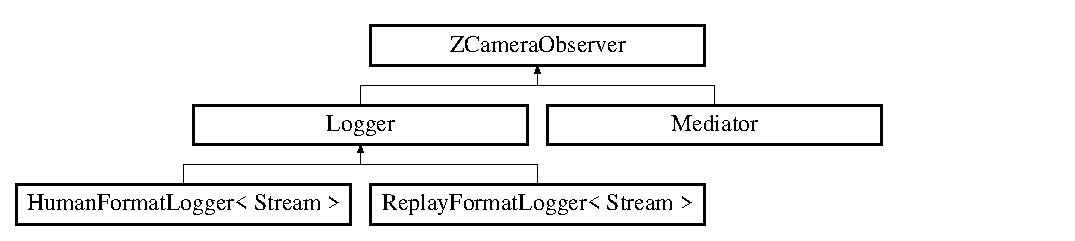
\includegraphics[height=2.78607cm]{classZCameraObserver}
\end{center}
\end{figure}
\subsection*{Public Member Functions}
\begin{DoxyCompactItemize}
\item 
\hypertarget{classZCameraObserver_a627e480f25c0d2ef0407f6b09e6883d4}{
virtual void {\bfseries update} (ZCameraUpdateContext context, const void $\ast$data)=0}
\label{classZCameraObserver_a627e480f25c0d2ef0407f6b09e6883d4}

\end{DoxyCompactItemize}


The documentation for this class was generated from the following files:\begin{DoxyCompactItemize}
\item 
/home/kevin/workspace/HugMe/HugMe v0.9.1/ZCamera/ZCameraObserver.h\item 
/home/kevin/workspace/HugMe/HugMe v0.9.1/ZCamera/ZCameraObserver.cpp\end{DoxyCompactItemize}

\hypertarget{classZCameraReplayer}{
\section{ZCameraReplayer Class Reference}
\label{classZCameraReplayer}\index{ZCameraReplayer@{ZCameraReplayer}}
}
Inheritance diagram for ZCameraReplayer:\begin{figure}[H]
\begin{center}
\leavevmode
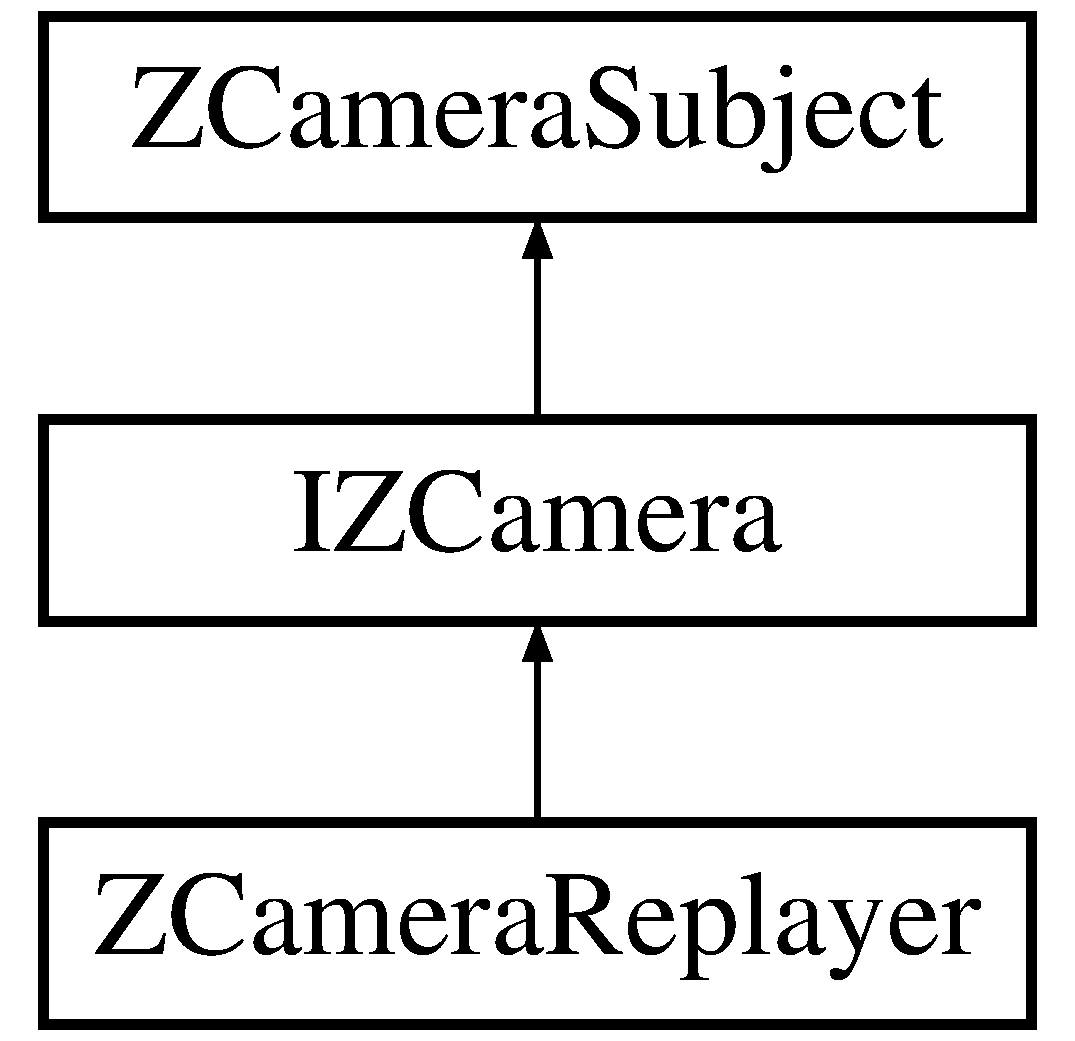
\includegraphics[height=3.000000cm]{classZCameraReplayer}
\end{center}
\end{figure}
\subsection*{Public Member Functions}
\begin{DoxyCompactItemize}
\item 
\hypertarget{classZCameraReplayer_a3cf08f3105a04e6cb143f762a55bafd5}{
{\bfseries ZCameraReplayer} (boost::shared\_\-ptr$<$ std::ifstream $>$ file, boost::shared\_\-ptr$<$ boost::archive::text\_\-iarchive $>$ archive)}
\label{classZCameraReplayer_a3cf08f3105a04e6cb143f762a55bafd5}

\item 
\hypertarget{classZCameraReplayer_af867b41ba331deca1e88c6b6ded547e6}{
void {\bfseries replay} (LogEvent\_\-t logEvent)}
\label{classZCameraReplayer_af867b41ba331deca1e88c6b6ded547e6}

\item 
\hypertarget{classZCameraReplayer_aa5ac01ea8f9f47b51cf92ad0aa0d7fc4}{
virtual void {\bfseries startCapture} ()}
\label{classZCameraReplayer_aa5ac01ea8f9f47b51cf92ad0aa0d7fc4}

\item 
\hypertarget{classZCameraReplayer_af25eba02746ce6c8f4765c6466c3841e}{
virtual void {\bfseries stopCapture} ()}
\label{classZCameraReplayer_af25eba02746ce6c8f4765c6466c3841e}

\end{DoxyCompactItemize}


The documentation for this class was generated from the following files:\begin{DoxyCompactItemize}
\item 
/home/kevin/workspace/HugMe/HugMe v0.9.1/Replay/ZCameraReplayer.h\item 
/home/kevin/workspace/HugMe/HugMe v0.9.1/Replay/ZCameraReplayer.cpp\end{DoxyCompactItemize}

\hypertarget{classZCameraSubject}{
\section{ZCameraSubject Class Reference}
\label{classZCameraSubject}\index{ZCameraSubject@{ZCameraSubject}}
}
Inheritance diagram for ZCameraSubject:\begin{figure}[H]
\begin{center}
\leavevmode
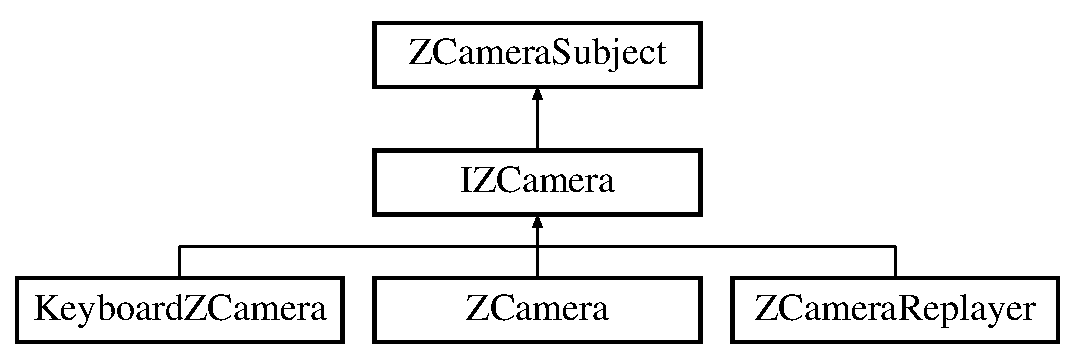
\includegraphics[height=3.000000cm]{classZCameraSubject}
\end{center}
\end{figure}
\subsection*{Public Member Functions}
\begin{DoxyCompactItemize}
\item 
\hypertarget{classZCameraSubject_a03a7bde4d7455c415bed12941121f304}{
void {\bfseries attach} (\hyperlink{classZCameraObserver}{ZCameraObserver} $\ast$observer)}
\label{classZCameraSubject_a03a7bde4d7455c415bed12941121f304}

\item 
\hypertarget{classZCameraSubject_acdcf65ddc2d3ea93d0b2012b095b0ed1}{
void {\bfseries detach} (\hyperlink{classZCameraObserver}{ZCameraObserver} $\ast$observer)}
\label{classZCameraSubject_acdcf65ddc2d3ea93d0b2012b095b0ed1}

\item 
\hypertarget{classZCameraSubject_a6c47d74ec2b13313052462250177f9e8}{
void {\bfseries notify} (ZCameraUpdateContext context, const void $\ast$data=NULL)}
\label{classZCameraSubject_a6c47d74ec2b13313052462250177f9e8}

\end{DoxyCompactItemize}


The documentation for this class was generated from the following files:\begin{DoxyCompactItemize}
\item 
/home/kevin/workspace/HugMe/HugMe v0.9.1/ZCamera/ZCameraSubject.h\item 
/home/kevin/workspace/HugMe/HugMe v0.9.1/ZCamera/ZCameraSubject.cpp\end{DoxyCompactItemize}

\printindex
\end{document}
